% ======================================================================
%  Witten, Three Lectures On Topological Phases Of Matter
%  中文译注本主文件
%  编译：xelatex 1510.07698v2(1)_中文译注.tex（两遍）
% ======================================================================
% ======================================================================
%  Witten, Three Lectures On Topological Phases Of Matter
%  中文译注本导言区
%  编译：xelatex（两遍），UTF-8
% ======================================================================
\documentclass[11pt,a4paper]{article}

\usepackage[UTF8,scheme=chinese,fontset=fandol]{ctex}
\usepackage{amsmath,amssymb,amsfonts,mathrsfs}
\usepackage{slashed}
\usepackage{graphicx}
\usepackage{booktabs}
\usepackage{geometry}
\usepackage{caption}
\usepackage{xcolor}
\usepackage{hyperref}

\geometry{left=2.4cm,right=2.4cm,top=2.5cm,bottom=2.5cm}
\graphicspath{{figures/}{./}}
\linespread{1.12}
\setlength{\parindent}{2em}
\setlength{\parskip}{0.15em}
\emergencystretch=2.5em

\numberwithin{equation}{section}

\captionsetup{font=small,labelfont=bf,labelsep=period}
\hypersetup{
  colorlinks=true,
  linkcolor=blue!45!black,
  citecolor=green!35!black,
  urlcolor=blue!55!black,
  pdftitle={物质的拓扑相三讲（Witten）},
  pdfauthor={Edward Witten；中文译注}
}

% ----------------------------------------------------------------------
%  原文的自定义宏（保留原语义；仅把依赖特殊字体的少数宏改为标准写法）
% ----------------------------------------------------------------------
\def\veps{\varepsilon}
\def\eps{\epsilon}
\def\eff{{\mathrm{eff}}}
\def\h{\widehat}
\def\U{{\mathrm U}}
\def\ang{\vartheta}
\def\bp{\begin{pmatrix}}
\def\ep{\end{pmatrix}}
\def\sR{{\mathsf R}}
\def\sT{{\mathsf T}}
\def\sP{{\mathsf P}}
\def\sPT{{\mathsf{PT}}}
\def\HH{{\mathfrak H}}
\def\ICS{{\mathrm{CS}}}
\def\CS{{\mathrm{CS}}}
\def\bea{\begin{array}}
\def\eea{\end{array}}
\def\beq{\begin{equation}}
\def\eeq{\end{equation}}
\def\beqn{\begin{eqnarray}}
\def\eeqn{\end{eqnarray}}
\def\tr{{\mathrm{tr}}}
\def\Tr{{\mathrm{Tr}}}
\def\Str{{\mathrm{STr}}}
\def\nnr{\nonumber\\}
\def\ex{{\mathrm e}}
\def\B{\mathcal B}
\def\T{\theta}
\def\G{\Gamma}
\def\D{\delta}
\def\P{\Phi}
\def\L{\mathcal L}
\def\K{\kappa}
\def\bzeta{\bar{\zeta}}
\def\CC{\mathbf C}
\def\RR{\mathbf R}
\def\ZZ{\mathbf Z}
\def\Z{\mathbf Z}
\def\fr{\frac}
\def\pt{\partial}
\def\cN{\mathcal N}
\def\cA{\mathcal A}
\def\cB{\mathcal B}
\def\rmd{\mathrm{d}}
\def\d{{\mathrm d}}
\def\dA{\dot{A}}
\def\dB{\dot{B}}
\def\dC{\dot{C}}
\def\dD{\dot{D}}
\def\da{\dot{a}}
\def\db{\dot{b}}
\def\bZ{\bar{Z}}
\def\bz{\bar{z}}
\def\calK{\mathcal K}
\def\SG{SG}
\def\sg{\mathfrak{sg}}
\def\gbos{\mathfrak{g}_{\bar{0}}}
\def\gferm{\mathfrak{g}_{\bar{1}}}
\def\gleft{\mathfrak{g}_\ell}
\def\gright{\mathfrak{g}_r}
\def\Dbos{\Delta^+_{\bar{0}}}
\def\Dferm{\Delta^+_{\bar{1}}}
\def\DfermI{\bar{\Delta}^+_{\bar{1}}}
\def\bos{{\bar{0}}}
\def\ferm{{\bar{1}}}
\def\osp{\mathfrak{osp}}
\def\sp{\mathfrak{sp}}
\def\so{\mathfrak{so}}
\def\hyp{{\mathrm{hyp}}}
\def\mj{{\mathrm{j}}}
\def\sign{\operatorname{sign}}
\def\SO{\mathrm{SO}}
\def\Sp{\mathrm{Sp}}
\def\SU{\mathrm{SU}}
\def\frak{\mathfrak}
\def\cL{\mathcal{L}}
\def\cO{\mathcal{O}}
\def\F{\mathcal F}
\def\C{\mathbf C}
\def\Gr{\mathrm{Gr}}
\def\bg{\overline\gamma}
\def\g{\gamma}
\def\bar{\overline}
\def\OSp{\mathrm{OSp}}
\def\Spin{\mathrm{Spin}}
\def\hat{\widehat}
\def\S{\mathcal S}
\def\Bbb{\mathbb}
\def\A{\mathcal A}
\def\i{\mathrm i}
\def\p{\mathbf p}
\def\q{\mathbf q}
\def\AA{\mathcal A}
\def\NN{\mathfrak N}
\def\N{\mathcal N}
\def\YM{\mathrm{YM}}
\def\tilde{\widetilde}
\def\t{\tilde}
\def\DD{\mathcal D}
\def\u{\mathfrak u}
\def\R{\mathcal R}
\def\2{\mathbf 2}
\def\1{\mathbf 1}
\def\0{\mathbf 0}
\def\s{\mathbf s}
\def\Q{Q}
\def\cQ{\mathcal{Q}}
\def\fsigma{\xi}
\def\Pexp{P\hspace{-0.7mm}\exp}
\def\ta{\widetilde{a}}
\def\bft{\mathbf t}
\def\afg{\hat{\mathfrak g}}
\def\be{\begin{equation}}
\def\ee{\end{equation}}
\def\H{\mathcal H}
\def\W{\mathcal W}
\def\V{\mathcal V}
\def\O{\mathcal O}
\def\J{\mathcal J}
\def\Qb{Q}
\def\cAb{\mathcal A_{b}}
\def\cAf{\mathcal A_{f}}
\def\cFb{\mathcal F_{b}}
\def\cDb{\mathcal D_{b}}
\def\Nb{N}
\def\psit{\psi_t}
\def\psiw{\psi_w}
\def\chit{\chi_t}

% ----------------------------------------------------------------------
%  “本节重点”环境
% ----------------------------------------------------------------------
\newenvironment{keytakeaways}
  {\par\medskip\noindent\textbf{本节重点}\begin{itemize}\small}
  {\end{itemize}\par\medskip}

% 图注中的“原文位置”用小字
\newcommand{\figloc}[2]{%
  \\[2pt]{\footnotesize 原文位置：Fig.~#1（PDF 第~#2~页）}}

% 引用与脚注中的中文
\renewcommand{\refname}{参考文献}
\renewcommand{\figurename}{图}
\renewcommand{\tablename}{表}
\renewcommand{\contentsname}{目\hspace{1em}录}


\begin{document}

% ======================================================================
%  标题页、摘要、目录、译注说明、引言
% ======================================================================
\begin{titlepage}
  \centering
  \vspace*{2.2cm}

  {\LARGE\bfseries 物质的拓扑相三讲\par}

  \vspace{1.6cm}

  {\large Edward Witten\par}

  \vspace{0.8cm}

  {\small 普林斯顿高等研究院自然科学学院\\
  普林斯顿，新泽西州 08540\par}

  \vspace{1.8cm}

  {\small arXiv:1510.07698v2\quad [cond-mat.mes-hall]\quad 2016 年 6 月 13 日\par}

  \vspace{0.4cm}

  {\small 原载 \textit{La Rivista del Nuovo Cimento} \textbf{39} (2016) 313--370\par}

  \vfill

  \begin{minipage}{0.86\textwidth}
    \small
    \noindent\textbf{摘要}\quad
    这些讲稿基于 2015 年 7 月在普林斯顿大学与高等研究院举办的
    PSSCMP/PiTP 暑期学校上的讲座。内容主要讨论那些可以用自由费米子和
    能带理论理解的物质拓扑相。文中还从有效场论的观点对分数量子霍尔效应
    作了介绍。
  \end{minipage}

  \vspace{1.2cm}
\end{titlepage}

\thispagestyle{empty}
\tableofcontents
\clearpage

\setcounter{page}{1}
\setcounter{section}{-1}

\section*{译注说明}
\addcontentsline{toc}{section}{译注说明}

\begin{enumerate}
  \item \textbf{底本。}译文依据 arXiv:1510.07698v2（2016 年 6 月 13 日版，
        60 页）与作者提供的 LaTeX 源文件；原文后发表于
        \textit{La Rivista del Nuovo Cimento} \textbf{39} (2016) 313--370。
        文中公式编号、图号、节号均沿用原文，以便与原文对照。

  \item \textbf{公式。}所有行内、行间公式均按原 LaTeX 源逐字符保留，包括指标位置、
        上下标、希腊字母、归一化因子与符号约定；译文未擅自“修正”任何公式。
        若发现原文笔误或可疑之处，以源码中的 Tutor Note 注释形式
        写在源码中，正文保持原样。源文件中的这类批注不进入 PDF。

  \item \textbf{术语。}以中文学界通行译名为准，例如 gauge theory 译“规范场论”，
        holonomy 译“和乐”，anomaly 译“反常”，Berry connection 译“贝里联络”。
        主要术语见随附《术语表》。

  \item \textbf{批注。}源码中含有三类学术批注：\textbf{易错}（张量缩并、指标升降、
        符号与归一化约定）、\textbf{含糊}（作者以“显然”“标准结果”跳过之处）、
        \textbf{笔误}（原文明显的排版或符号错误）。批注均尽量具体到公式号、图号、
        节号或文献键，供教授对照原文核读。

  \item \textbf{图。}原文 43 幅图均从作者源文件提取，按原编号插入；
        图注译为中文，并以小字附原文图号与 PDF 页码。图内文字保留原文，
        以便与原文图直接比对。

  \item \textbf{编译。}本文件使用 XeLaTeX{} 编译（两遍），文档类为
        \texttt{article}，中文由 \texttt{ctex} 宏包的 Fandol 字体集排版。
        编译命令：\texttt{xelatex 1510.07698v2(1)\_中文译注.tex}，重复两遍。
\end{enumerate}

\clearpage

\section{引言}

\begin{keytakeaways}
  \item 本讲稿的范围：用自由费米子与能带拓扑理解物质相，并以有效场论简介分数量子霍尔效应。
  \item 主线：能带交叉的拓扑稳定性（缠绕数、贝里联络、陈类）$\rightarrow$ 外尔半金属与拓扑绝缘体
        $\rightarrow$ 陈-西蒙斯有效作用量与量子霍尔效应。
  \item 方法：把拓扑不变量同时用同伦群、微分形式与纤维丛三种语言表述，便于与场论/数学工具对接。
  \item 阅读提示：第一讲偏能带与拓扑，第二讲偏有效场论，第三讲回到分数量子霍尔效应与具体模型；
        公式编号沿用原文，便于对照。
\end{keytakeaways}

近年来，量子场论在凝聚态物理中发现了若干引人入胜的新应用。文献入门可参见综述文章
\cite{KH,ZQ,MZ} 与专著 \cite{BH}。

本讲稿基于我 2015 年 7 月在普林斯顿大学与高等研究院的 PSSCMP/PiTP 暑期学校所作四次讲座中的
前三讲。这些讲座几乎没有新意；我只是解释了自己对这个迷人主题所能理解的部分。
（第四讲确有一些新内容，已另行成文 \cite{Witten}。）参考文献列出了一些经典的和较新的论文，
但当然并不完整。

在这些讲座中，我主要集中于可用\textbf{非相互作用电子}与\textbf{拓扑能带理论}理解的物质相。
主要的例外是对分数量子霍尔效应某些方面的简短介绍。

本讲稿大体上紧循原讲座；少数主题略作调整，并补充了原讲座中因时间不够而未能涉及的若干内容。
这里讨论的一些主题，暑期学校的其他讲者（尤其是 Charlie Kane 与 Nick Read）曾从不同观点作过阐述。


% ======================================================================
%  第一讲　自由费米子与能带拓扑（1.1-1.4）
% ======================================================================
\section{第一讲}

\begin{keytakeaways}
  \item 一维晶体中单带色散一般以非零斜率穿过费米能，线性化后即得相对论性的
        无质量手征费米子；但动量的周期性要求向上穿过与向下穿过的次数相等，
        故左行模与右行模一样多，这正是 1+1 维阿德勒-贝尔-杰基夫反常相消的
        拓扑根源。
  \item 三维中一般的两带哈密顿量由泡利矩阵的三个实系数刻画，能级简并相当于
        三个实条件，因此能带交叉在三维中是普遍现象；在交叉点附近展开即得
        手征狄拉克（外尔）哈密顿量，其手征性由能带映射的三阶雅可比行列式的
        符号给出。
  \item 每个坏点可用“包围它的小球面到单位球面的映射的度”即缠绕数来标记；
        尼尔森-二宫定理断言所有坏点的缠绕数之和为零，故正、负手征性的无能隙模
        成对出现，从而保证规范不变性不被破坏。
  \item 该定理有三种等价证明：同伦群与积分公式、闭 2-形式的斯托克斯定理、
        以及填充态复线丛的贝里联络与第一陈类；其中曲率在坏点小球面上的通量
        恰等于缠绕数。
  \item 填充态构成布里渊区上的复线丛，其贝里联络一般不平坦，曲率除以 $2\pi$
        即第一陈类；这套“能带拓扑”语言是第二讲陈-西蒙斯有效作用量、
        第三讲量子霍尔效应讨论的共同基础。
\end{keytakeaways}

\subsection{一维空间中的相对论色散}

我们先问：在什么条件下，才应当期望在晶体中发现电子的相对论性色散关系？
在一维空间中，答案是熟悉的。记单粒子能量 $\veps$ 作为动量 $p$ 的函数为 $\veps(p)$；
一般地，$\veps(p)$ 会在某个 $p=p_0$ 处以非零斜率穿过费米能（图~\ref{cigar}）。

\begin{figure}
 \begin{center}
   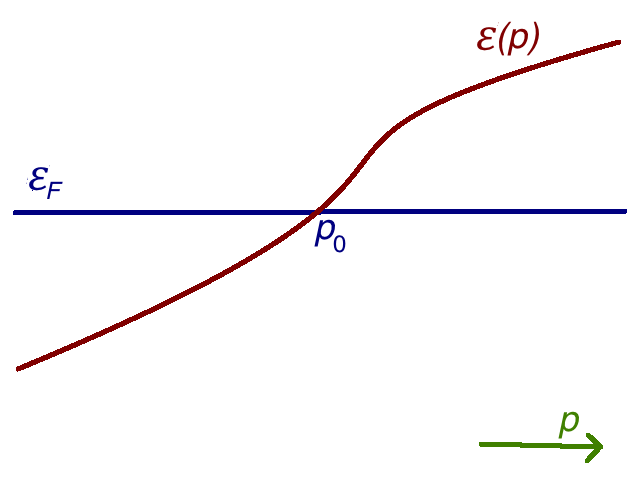
\includegraphics[width=3in]{OneDimFermi2.png}
 \end{center}
\caption{\small  在一维中，单粒子能量 $\veps(p)$ 一般地在某个孤立动量 $p_0$ 处穿过费米能。\figloc{1}{3}}
 \label{cigar}
\end{figure}

% [Tutor Note: 易错——式 (\ref{dolz}) 的线性化以 $v=\partial\veps/\partial p\neq0$ 为前提，$v$ 即能带群速度；若晶体有反射或时间反演对称性迫使 $\veps(p)$ 在交点处取极值（斜率恰为零），则一阶项消失，式 (\ref{dolz}) 失效，能带在该点表现为二次接触（并不自动打开能隙）。原文所说的“一般地”正是排除这类特殊对称性。]
于是，把色散关系在 $p=p_0$ 附近线性化，得到
\begin{equation}\label{dolz}\veps=\veps(p_0)+v(p-p_0)+\O((p-p_0)^2),~~~ v=\left.\frac{\partial \veps}{\partial p}\right|_{p=p_0}.\end{equation}
除开一个可加常数 $\veps(p_0)$ 与平移 $p\to p-p_0$ 之外，这就是一个相对论性色散关系，
类似于 $\veps=cp$，只是光速 $c$ 被替换为 $v$。当 $v>0$（$v<0$）时，
位于 $p=p_0$ 附近的无能隙模向右（向左）传播。

% [Tutor Note: 易错——式 (\ref{continuum}) 用 $-i\partial/\partial x$ 表示 $p-p_0$，隐含取 $\hbar=1$（恢复 $\hbar$ 时应为 $-i\hbar\partial_x-p_0$）；式 (\ref{constantshift}) 中的 $\veps(p_0)\int\psi^*\psi$ 只是整体化学势的平移，不影响激发谱，故后文可以略去。]
描述 $p=p_0$ 附近诸模的相应连续模型是
\begin{equation}\label{continuum} H=v\int_{-\infty}^\infty \d x \,\,\psi^*\left(-\i\frac{\partial}{\partial x}\right)\psi.\end{equation}
这是一维手征费米子的相对论作用量，只不过 $v$ 取代了 $c$，
而 $-i\partial/\partial x$ 代表的是 $p-p_0$ 而非 $p$。此外，我们在 $H$ 中略去了每粒子的
“常数” $\veps(p_0)$：
\be\label{constantshift}\veps(p_0)\int_{-\infty}^\infty \d x \,\psi^*\psi.\ee

% [Tutor Note: 含糊——“向上穿过与向下穿过次数相等”其实只是 $\veps(p)$ 在圆周（一维布里渊区）上单值的初等推论：从下方穿出一次，必在另一处从上方穿回。不要把它拔高为 $\pi_1(S^1)$ 的缠绕数论证，也不要与 1.3 节 $\pi_2(S^2)\cong\Z$ 的坏点缠绕数求和混为一谈；二者的拓扑对象不同。$1+1$ 维手征反常见 \cite{Adler,BJ}，格点上的阻碍见 \cite{NN,F}。]
这个一维情形给出了一个简明的首例，说明拓扑中的整体性条件如何限制我们所能得到的
低能场论——以及这些限制如何常常映照出相对论场论与“反常”中熟知的事实。
我们必须记住：在晶体的语境中，动量 $p$ 是周期变量。
由于 $\veps(p)$ 是周期的，由此可知（图~\ref{Crossings}）：每当 $\veps(p)$ 从下方穿过
费米能 $\veps_F$ 一次，就还有另一次它从上方穿过 $\veps_F$。
所以实际上，无能隙的左行费米子模与右行费米子模一样多。

% [Tutor Note: 笔误——图 \ref{Crossings} 的图注中，第一处费米能写作 $\eps_F$（即 \verb|\epsilon|），第二处写作 $\veps_F$（即 \verb|\varepsilon|），同一个量用了两种字形；正文一律用 $\veps_F$。译文照原样保留，排版时可视需要统一。]
\begin{figure}
 \begin{center}
   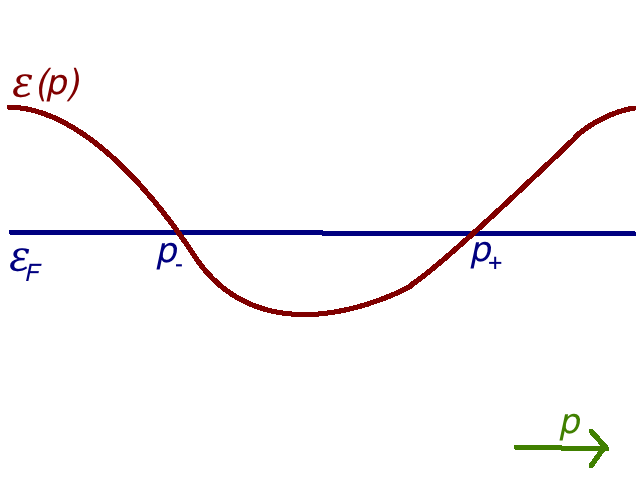
\includegraphics[width=3in]{Crossings.png}
 \end{center}
\caption{\small  在一维中，对每一个使 $\veps(p)$ 上升到 $\eps_F$ 之上的动量值，
都存在另一点使它下降到 $\veps_F$ 之下。\figloc{2}{4}}
 \label{Crossings}
\end{figure}

% [Tutor Note: 易错——式 (\ref{hamdir}) 下方定义的 $\bar\gamma=\gamma_0\gamma_1$ 用的是下指标；在 $\eta_{\mu\nu}=\mathrm{diag}(-1,1)$ 下 $\gamma_0=-\gamma^0$，故 $\bar\gamma=-\gamma^0\gamma^1$。“正手征=右行”这一对应依赖此符号约定：若改用 $\gamma^0\gamma^1$ 作手征算符，则左右行与正负手征性的对应整体对调。]
% [Tutor Note: 术语——手征性（chirality）指手征算符的本征值（此处为 $\bar\gamma$，$3+1$ 维中为 $\gamma_5$），是洛伦兹不变量；螺旋度（helicity）指自旋沿动量方向的投影，只有对无质量粒子才是洛伦兹不变量，有质量时依赖参考系。无质量时二者一致（差一符号约定），见本段末的脚注。]
用相对论的术语说，右行模与左行模分别被称为具有正手征性与负手征性。
这一术语的由来是：2 维时空中的无质量狄拉克方程为
\be\label{Dirac}\left(\gamma^0\frac{\partial}{\partial t}+\gamma^1\frac{\partial}{\partial x}\right)\psi=0,\ee
其中 $\g^\mu$ 是狄拉克矩阵，满足克利福德代数关系
\be\label{gamma}\{\gamma^\mu,\gamma^\nu\}=2\eta^{\mu\nu},~~~~\eta_{\mu\nu}=\mathrm{diag}(-1,1).\ee
写成哈密顿量形式，狄拉克方程为
\be\label{hamdir}\i\frac{\partial\psi}{\partial t}= -\i\bar\gamma \frac{\partial\psi}{\partial x},\ee
其中 $\bar\gamma=\gamma_0\gamma_1$（它在 $3+1$ 维中的对应物通常称为 $\gamma_5$）是
“手征算符”。因此，正手征或负手征的费米子态分别就是右行或左行的。

% [Tutor Note: 含糊——作者说这一拓扑事实“使我们免于麻烦”，略去的是 $1+1$ 维阿德勒-贝尔-杰基夫（Adler-Bell-Jackiw）反常的实质：费米子测度在手征变换下不守恒，反常系数正比于 $n_+-n_-$，故 $n_+\neq n_-$ 时 $U(1)$ 规范不变性（进而电荷守恒）在量子层次失效。参见 \cite{Adler,BJ}。]
% [Tutor Note: 笔误——本段原文作“the 3d Nielson-Ninomiya theorem”，其中 Nielson 疑应为 Nielsen（见文献 \cite{NN}）；又 1.2 节首句“There is certainly more that one could say”中 that 疑应为 than。]
于是，对于无能隙的带电模，一个更现实的哈密顿量大致是
\be\label{realism}H=-v_-\int_{-\infty}^\infty \d x \,\,\psi_-^*\left(-\i\frac{\partial}{\partial x}\right)\psi_-+ 
v_+\int_{-\infty}^\infty \d x \,\,\psi_+^*\left(-\i\frac{\partial}{\partial x}\right)\psi_+,\ee
其中 $\psi_+$ 与 $\psi_-$ 是正、负手征性的模，且一般说来它们以不同的速度传播。
如果熟悉量子规范场论与反常，就会认识到：这一拓扑事实——它是三维
尼尔森-二宫（Nielsen-Ninomiya）定理的一维类比，我们马上就要讲到后者——
使我们免于麻烦。一个纯粹 $1+1$ 维的理论，比如含有 $n_+$ 个右行无能隙电子模与
$n_-$ 个左行模，是“反常的”；也就是说，它不具备规范不变性，也不守恒电荷——
除非 $n_+=n_-$。这个反常是阿德勒-贝尔-杰基夫（Adler-Bell-Jackiw）反常的
$1+1$ 维版本 \cite{Adler,BJ}，后者在粒子物理中非常重要。

% [Tutor Note: 易错——图 \ref{Crossings} 中的 $p_+$ 与 $p_-$ 指 $\veps(p)$ 穿过 $\veps_F$ 的两个动量位置（原文未显式定义）：$p_+$ 处能带自下而上穿出，$p_-$ 处自上而下穿入。$\d p/\d t>0$ 时电子沿 $+p$ 方向漂移，在 $p_+$ 处堆积电子、在 $p_-$ 处留下空穴，故单支电荷不守恒而总电荷守恒；若 $n_+\neq n_-$，净手征电荷随时间线性增长，这正是反常的表现。]
其实，只要重新审视图~\ref{Crossings}，并假定加上一个恒定电场，我们就能看到这个潜在的反常。
当电场的符号使得对每个电子都有 $\d p/\d t>0$ 时，所有电子都会在图中向右“流动”。
这会在 $p=p_+$ 处产生电子、在 $p=p_-$ 处产生空穴，于是 $p=p_+$ 模或 $p=p_-$ 模
所携带的电荷并不守恒，尽管总电荷当然是守恒的。
因此，电荷守恒要求两类模的数目相等。

\subsection{三维}

在一维空间中，当然还有更多可说的东西；但我们还是要转而讨论空间维度 3。
作为预备，回顾一下量子力学能级相互排斥：这意味着，若 $H(\lambda)$ 是一般的单参数
哈密顿量族，依赖于参数 $\lambda$ 且没有特定对称性，则一般地其能级不会作为
$\lambda$ 的函数相交（图~\ref{repel}）。
但是，赫尔林（Herring）曾追问：能级之间究竟相互排斥到什么程度？一般地，要调节多少个参数才能使两个
能级重合？

\begin{figure}
 \begin{center}
   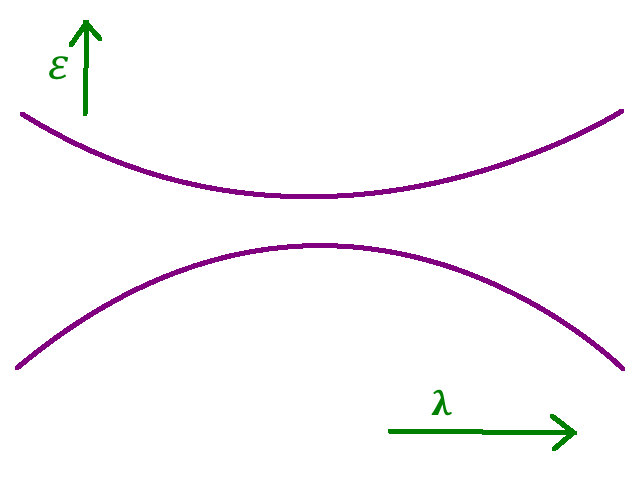
\includegraphics[width=2.5in]{Levels.png}
 \end{center}
\caption{\small  一般地，当参数变化时，量子力学能级不会相交。\figloc{3}{5}}
 \label{repel}
\end{figure}

% [Tutor Note: 含糊——“量子力学能级相互排斥”的定量内容是 von Neumann-Wigner 定理：无对称性时，两个能级简并的余维数为 3，即一般需要调节 3 个参数。作者引 \cite{Herring} 正是把这一计数用于晶体能带的“偶然简并”，回答“要调几个参数”。]
% [Tutor Note: 易错——式 (\ref{generic})-(\ref{ecial}) 的参数计数：$a,c$ 为实、$b$ 为复，共 4 个实参数；简并条件 $\vec b=0$ 是 3 个实条件，剩下的 1 个参数是共同本征值。注意后文可用 $c$-数函数把 $a(p)$ 减掉，故真正控制交叉的只是 $\vec b(p)$ 的三个分量。另：原文式标签 specil、ecial、expa、xpa 拼写不整（疑为 special、especial、expansion 之残），因不影响交叉引用，译文照原样保留。]
这个问题的答案是：必须调节 3 个实参数。因为一个一般的 $2\times 2$ 厄米矩阵依赖于
4 个实参数
\be\label{generic} H=\begin{pmatrix} a & b \cr \bar b & c\end{pmatrix} , \ee
而能级相等的 $2\times 2$ 厄米矩阵只依赖于 1 个实参数
\be\label{specil}H = \begin{pmatrix} a & 0 \cr 0 & a \end{pmatrix}.\ee
换一种说法，任何 $2\times 2$ 厄米矩阵都可写成
\be\label{ecial}H = a+\vec b\cdot \vec \sigma,\ee
其中 $\vec\sigma$ 是泡利矩阵。$H$ 具有相等本征值的条件是 $\vec b=0$，
这是三个实条件。

% [Tutor Note: 易错——式 (\ref{expa}) 中 $b_{ij}=\partial b_i/\partial p_j$ 是 $3\times3$ 实雅可比矩阵；式 (\ref{xpa}) 的缩并是 $\sigma_i b_{ij}(p-p_*)_j$，即 $\sigma$ 与下标 $i$ 缩并、动量差与下标 $j$ 缩并。式 (\ref{perd}) 用该矩阵行列式的符号定义手征性，故要求 $b_{ij}$ 非奇异，否则该点不是孤立的 $\pm1$ 坏点。]
在三维中，能带哈密顿量 $H(p_1,p_2,p_3)$ 依赖于三个实参数，因此两条能带在某个
孤立值 $p=p_*$ 处交叉是很自然的。在 $p=p_*$ 附近，且只看所涉及的两条能带，
哈密顿量大致形如
\be\label{localexp}H=a( p)+ \vec b( p)\cdot \vec\sigma,\ee
其中在 $p=p_*$ 处 $\vec b(p)=0$。在 $p=p_*$ 附近展开，
\be\label{expa}b_i(p)=\sum_j b_{ij} (p-p_*)_j+\O((p-p_*)^2),~~ b_{ij}= \left.\frac{\partial b_i}{\partial p_j}\right|_{p=p_*}.\ee
于是，略去一个常数并忽略高阶项后，能带劈裂在 $p=p_*$ 附近由下式描述：
\be\label{xpa}H'=\sum_{i,j}\sigma_i b_{ij}(p-p_*)_j.\ee

% [Tutor Note: 术语——式 (\ref{thred})、(\ref{hameq}) 取 $\eta_{\mu\nu}=\mathrm{diag}(-1,1,1,1)$，此时 $\gamma_0=-\gamma^0$，故 $\gamma_0\gamma_k=-\gamma^0\gamma^k$。原文随后写 $\gamma_5=\i\gamma_0\gamma_1\gamma_2\gamma_3$（下指标），又用括注恒等式 $\gamma_0\gamma_1\gamma_0\gamma_2=\i\gamma_0\gamma_3\gamma_5$；按此约定直接计算实得 $\gamma_0\gamma_1\gamma_0\gamma_2=\gamma_1\gamma_2=-\i\gamma_0\gamma_3\gamma_5$，与括注相差一负号。若改用 $\gamma_5=\i\gamma^0\gamma^1\gamma^2\gamma^3$（上指标），符号即一致。问题不在于“$\g$ 能否取实”——在 mostly-plus 的 Majorana 表示中 $\gamma^\mu$ 同样可以全取实矩阵——而在于全文须固定 $\gamma_5$ 用上指标还是下指标，并据此统一重核式 (\ref{sigmam})-(\ref{news}) 的符号。]

除开平移 $p\to p-p_*$，这本质上就是 $3+1$ 维中的手征狄拉克哈密顿量。
让我们回顾这一事实。$3+1$ 维中的无质量狄拉克方程是
\be\label{thred}\sum_{\mu=0}^3\gamma^\mu\partial_\mu\psi=0,~~~ \{\gamma^\mu,\gamma^\nu\}=2\eta^{\mu\nu},~~~~\eta_{\mu\nu}=\mathrm{diag}(-1,1,1,1).\ee
写成哈密顿量形式，该方程为
\be\label{hameq}\i\frac{\partial\psi}{\partial t}=-\i\sum_k\gamma_0\gamma_k \frac{\partial\psi}{\partial x^k}.  \ee
要表示四个伽马矩阵，我们需要 $4\times 4$ 矩阵（可以选为实矩阵）。
然而，矩阵
\be\label{chirm}\gamma_5=\i\gamma_0\gamma_1\gamma_2\gamma_3\ee 是洛伦兹不变的。
它满足 $\gamma_5^2=1$，故本征值为 $\pm 1$。
我们可以对 $\psi$ 施加一个“手征条件” $\gamma_5\psi=\pm \psi$，从而约化为一个
$2\times 2$ 狄拉克哈密顿量。但这样一来，由于 $\gamma_5$ 定义中的因子 $\i$，
且与 $1+1$ 维中的情形相反，$\psi$ 的伴随满足相反的手征条件。

一旦约化到 $\gamma_5\psi=\pm\psi$ 的手征 $2\times 2$ 狄拉克哈密顿量，出现在狄拉克
哈密顿量中的矩阵 $\gamma_0\gamma_i$ 便是 $2\times 2$ 厄米矩阵，我们可以把它们取为
（差一符号）泡利矩阵
\be\label{sigmam}\sigma_i=\pm \gamma_0\gamma_i.\ee
要点在于：若 $\gamma_5\psi=\pm \psi$，则{\it 在作用于 $\psi$ 时}，
\be\label{news}\sigma_i\sigma_j=\delta_{ij}+\i\epsilon_{ijk}\sigma_k.\ee
（对 $i=1,j=2$，可由显式恒等式
$\gamma_0\gamma_1\gamma_0\gamma_2=\i\gamma_0\gamma_3\gamma_5$ 证明。一般情形随后由
旋转对称性得到。）

于是，狄拉克哈密顿量
\be\label{dirha}  H=-\i\sum_k\gamma_{0}\gamma_k\frac{\partial}{\partial x^k} \ee
对于手征费米子变成
\be\label{irha} H=\mp \i c\sum_k\sigma^k\frac{\partial}{\partial x^k}=\pm c\,\vec\sigma\cdot \vec p.\ee   
符号取决于费米子的手征性，而正是它决定了我们在式 (\ref{sigmam}) 中必须选取哪个符号。
（这里我恢复了光速 $c$。）就术语而言，具有确定手征性——换言之，具有确定的
$\gamma_5$ 值——的带电相对论性费米子称为外尔（Weyl）费米子。
$\gamma_5$ 本征值的物理意义在于，它决定了费米子的“螺旋度”（自旋沿运动方向的
分量）。注意，“螺旋度”只有对{\it 无质量}粒子才是洛伦兹不变的概念
（无质量粒子在任何洛伦兹系中都不静止），而我们的出发点确实就是无质量狄拉克方程。
反粒子——可以把它想象为狄拉克海中的一个空穴——具有相反的螺旋度，\footnote{这种情况
之所以发生，是因为——与 $1+1$ 维中的情形相反——若 $\gamma^\mu$ 为实矩阵，则手征算符
$\g_5$ 为虚的。因此 $\psi$ 与其厄米伴随满足相反的手征条件。粒子物理中最基本的例子
是：在近似认为无质量的情形下，中微子与反中微子具有相反的螺旋度。}
正如它带有相反的电荷一样。式 (\ref{irha}) 的手征狄拉克哈密顿量描述了两条
$E=\pm c|p|$ 的能带（图~\ref{twob}）。

\begin{figure}
 \begin{center}
   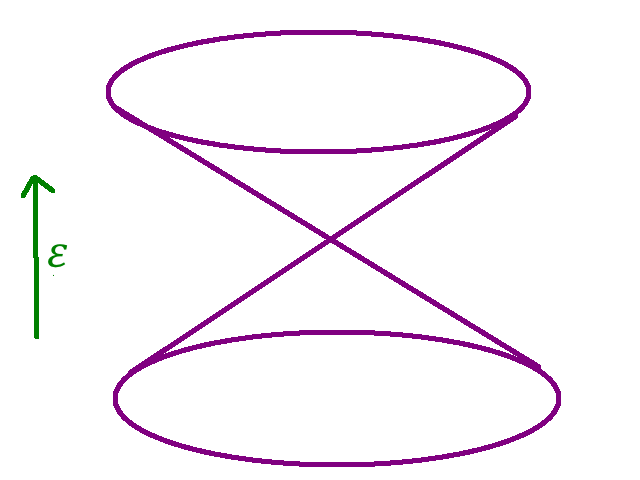
\includegraphics[width=2.5in]{TwoCrossing.png}
 \end{center}
\caption{\small  由手征狄拉克哈密顿量描述的一对能带。\figloc{4}{8}}
 \label{twob}
\end{figure}

因此，手征狄拉克哈密顿量基本上与我们为 $2\times 2$ 能带交叉所找到的一般哈密顿量
(\ref{xpa}) 相合，只需作替换 $cp_k\to \sum_j b_{kj}p_j$。
当然，这一替换意味着 $p=p_*$ 附近的费米子模并不以速度 $c$ 传播，而是慢得多。
此外，它们在 $\RR^3$ 上的标准欧几里得度规中也不必各向同性地传播。一般说来，
支配这些模的自然度规是
$$||p||^2=\sum_i\left(\sum_j b_{ij}p_j\right)^2.$$ 
换言之，有效度规为
$$G^{ij}=\sum_k b^i{}_kb^j{}_k.$$

% [Tutor Note: 易错——式 (\ref{perd}) 中 $\mathrm{sign}\det(b_{ij})$ 就是缠绕数的符号，其正负既依赖 $\sigma_i=\pm\gamma_0\gamma_i$ 的符号选择，也依赖动量空间定向（$\epsilon^{ijk}$ 以 $123$ 为正序）。原文取正行列式对应 $\gamma_5=+1$；若采用相反的 $\epsilon$ 约定，图 \ref{twoob} 中所有 $\pm$ 标记会同时反转，但“正负数目相等”的结论不变。]
% [Tutor Note: 笔误——本段“A gap crossing in which this determinant is positive”中 gap crossing 疑为 band crossing（能带交叉）；gap 指能隙，与文意相反。]
最后，也是非常重要的一点：无能隙电子模的{\it 手征性}由
\be\label{perd}\mathrm{sign}\,\det\left(b_{ij}\right)=\mathrm{sign}\,\det\left. \left(\frac{\partial b_i}{\partial p_j}\right)\right|_{p=p_*}. \ee
给出。若这一行列式为正（或负），则相应的能带交叉对应于 $\gamma_5=+1$
（或 $\gamma_5=-1$）的相对论性无质量手征费米子（或外尔费米子）。

\subsection{尼尔森-二宫定理}

然而现在，我们应当记住 $3+1$ 维相对论量子场论中的某些事实。一个 $U(1)$ 规范场
（电磁场）与一个只带单一手征性的无质量带电费米子耦合、而没有相反手征性的对应物时，
该理论是反常的：规范不变性在量子层次上失效，理论不自洽。
在 $1+1$ 维中，我们之所以避开了这样的矛盾，是因为一个简单的拓扑事实：
$\veps(p)$ 向下穿过费米能的次数与向上穿过的次数一样多，如图~\ref{Crossings} 所示。
一个类似的拓扑定理在 $3+1$ 维中解了围。这就是尼尔森-二宫定理 \cite{NN,F}，
它最初是作为相对论性手征费米子格点正规化的一个障碍而提出的。\footnote{尼尔森-二宫
定理所涉及的思想，与索利斯（Thouless）、科莫托（Kohmoto）、奈廷格尔（Nightingale）与
登奈斯（den Nijs）\cite{TKNN} 在量子霍尔效应方面著名工作中所发展的思想有些类似。
我们将在第二讲中介绍他们的结果。}

% [Tutor Note: 术语——“坏点”（bad point）指能带哈密顿量的能隙闭合点，即能带交叉点；文中与“外尔点”“狄拉克点”混用，含义随语境（两重简并 vs 多重简并）略有差别，译文按语境分别处理。]
在陈述这一定理时，我们假定能带哈密顿量 $H(p)$ 除布里渊区 $\B$ 中有限多个孤立点
之外处处有能隙（图~\ref{badp}）。我们将给每一个这样的坏点附上一个整数，
并证明这些整数之和为零。

\begin{figure}
 \begin{center}
   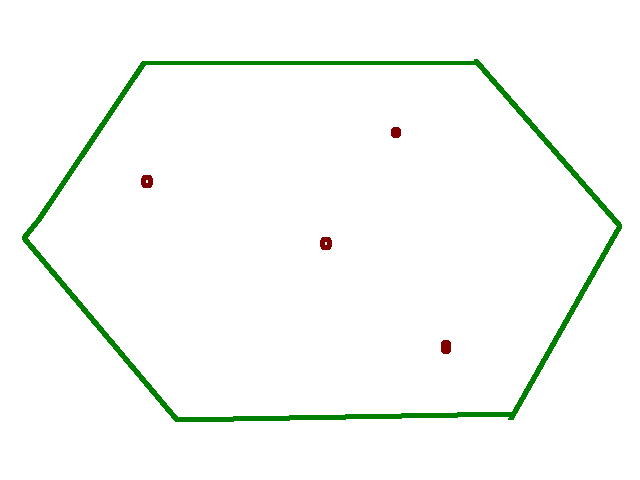
\includegraphics[width=2.5in]{BadPoints.png}
 \end{center}
\caption{\small  六边形内部象征布里渊区 $\B$。我们考虑一个除有限多个点之外处处有能隙的
能带哈密顿量，这些点由圆点标出。\figloc{5}{9}}
 \label{badp}
\end{figure}

首先，假定只有两条能带。此外，只需从 $H(p)$ 中减去一个关于 $p$ 的 $c$-数函数，
就能使 $H(p)$ 无迹，而不改变能带交叉。
于是
$$H(p)=\vec b(p) \cdot \vec \sigma$$
其中 $\vec b(p)$ 是某个向量值函数。现在，在坏点之外 $\vec b(p)\not=0$，因此可以定义
单位向量
$$\vec n(p) =\frac{\vec b}{|\vec b|}. $$
映射 $p\to \vec n(p)$ 在坏点之外有定义。我们想理解它的拓扑性质。

% [Tutor Note: 含糊——$\pi_d(S^d)\cong\Z$ 所说的“缠绕数”就是映射的度：$\deg\varphi=\int_{S^d}\varphi^*\eta$，其中 $\eta$ 是目标球面上总积分为 1 的体积形式。下文式 (\ref{wn}) 正是这一公式在 $d=2$ 时的具体化，其 $1/(4\pi)$ 来自单位球面积 $4\pi$。]
让我们只考虑其中一个坏点，比如位于 $p=p_*$ 的那个，并令 $S$ 是围绕该坏点的小球面
（图~\ref{sphere}）。映射 $p\to \vec n(p)$ 在 $S$ 上处处有定义。这是从一个二维球面——
即 $S$——到另一个二维球面——由单位向量 $\vec n$ 参数化——的映射。
我们把第二个二维球面记作 $S_{\vec n}$。在任何维数 $d$ 中，从一个 $d$ 维球面 $S^d$ 到
另一个同维球面的连续映射总有一个“缠绕数”或“包裹数”，即第一个球面绕第二个球面
缠绕的净次数。这反映了如下事实：
$$\pi_d(S^d)\cong\Z.$$

\begin{figure}
 \begin{center}
   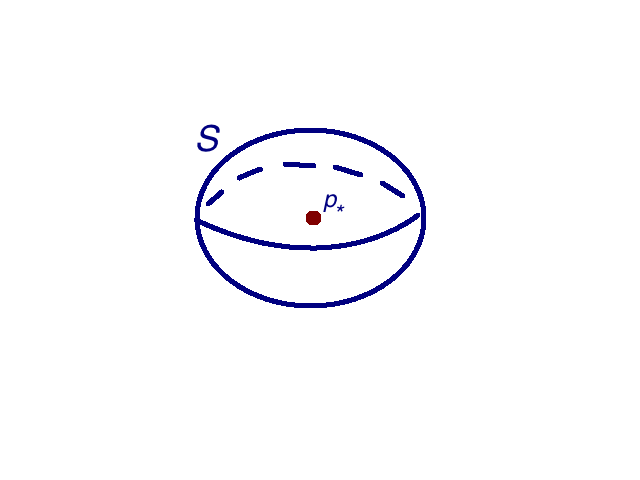
\includegraphics[width=3in]{Sphere.png}
 \end{center}
\caption{\small  围绕两能级交叉的坏点 $p_*$ 的小球面 $S$。\figloc{6}{9}}
 \label{sphere}
\end{figure}

在建立任何一般理论之前，让我们先看相对论性狄拉克哈密顿量
$H=\pm \vec \sigma\cdot \vec p,$
情形下的缠绕数，其中符号即费米子的手征性。
对该哈密顿量，$\vec b=\pm \vec p$，从而 $\vec n=\pm \vec p/|\vec p|$。
坏点是 $\vec p=0$，我们可以把围绕它的球面 $S$ 取为单位球面 $|\vec p|=1$。
于是从 $S$ 到 $S_{\vec n}$ 的映射就是
\be\label{zob}\vec n=\pm \vec p.\ee 
对 $+$ 手征性，这是恒等映射，缠绕数为 1；对 $-$ 手征性，它是负的恒等映射，
沿相反方向缠绕，缠绕数为 $-1$。

尼尔森-二宫定理断言：各坏点处缠绕数之和恒为零。一般地（在没有会导致更特殊行为的
晶格对称性时），绝对值大于 1 的坏点会分裂成若干个缠绕数为 $\pm 1$ 的坏点。
（我们在 \ref{somex} 节给出这一现象如何发生的显式例子。）因此一般地，所有坏点的
缠绕数都是 $\pm 1$，对应于一种或另一种手征性的无能隙外尔费米子。在这种情况下，
缠绕数之和为零意味着正、负手征性的无能隙模一样多，这正是相对论场论学家为保证
反常相消所期望的。

% [Tutor Note: 含糊——式 (\ref{wn}) 中的 $1/4\pi$ 来自单位球面积 $4\pi$；$\epsilon^{\mu\nu}$ 是二维反对称符号，$\d^2p$ 是球面 $S$ 上的面积元。式 (\ref{nwn}) 只是把 $\vec n\cdot(\partial_\mu\vec n\times\partial_\nu\vec n)$ 改写成 $\epsilon^{abc}n_a\partial_\mu n_b\partial_\nu n_c$，两式逐字等价。]
% [Tutor Note: 含糊——式 (\ref{zolf}) 的“右端为零”省去了展开细节：$\partial_\lambda$ 作用于后两个因子所得的项因 $\epsilon^{\lambda\mu\nu}$ 的反对称性而两两相消；剩下的 $\epsilon^{\lambda\mu\nu}\partial_\lambda\vec n\cdot(\partial_\mu\vec n\times\partial_\nu\vec n)$ 因三个向量均切于球面（与 $\vec n$ 正交，切空间为二维）而三重积为零。]
人们如何证明缠绕数之和为零？一种相当朴素的方法如下。
从 $S$ 到 $S_{\vec n}$ 的映射的缠绕数可以写成一个积分公式：
\be\label{wn}w(S)
=\frac{1}{4\pi}\int\d^2p\,\,\epsilon^{\mu\nu}\vec n\cdot \partial_\mu \vec n\times \partial_\nu \vec n.\ee
同一公式的等价写法是
\be\label{nwn}w(S)=\frac{1}{4\pi}\int_S\d^2 p\,\,\epsilon^{\mu\nu} \,\,\epsilon^{abc}n_a \frac{\partial n_b}{\partial p^\mu}\frac{\partial n_c}{\partial p^\nu}.\ee
现在
\be\label{zolf} 0=\partial_\lambda\left(\epsilon^{\lambda\mu\nu} \vec n\cdot \partial_\mu \vec n\times \partial_\nu \vec n\right),\ee
因为右端是 $\epsilon^{\lambda\mu\nu}\partial_\lambda \vec n\cdot \partial_\mu \vec n\times \partial _\nu \vec n$，
它为零，原因是它是三个矢量 $\partial_\lambda\vec n$、$\partial_\mu \vec n$ 与
$\partial_\nu\vec n$ 的三重叉积，而这三个矢量都垂直于球面 $|\vec n|=1$。

\begin{figure}
 \begin{center}
   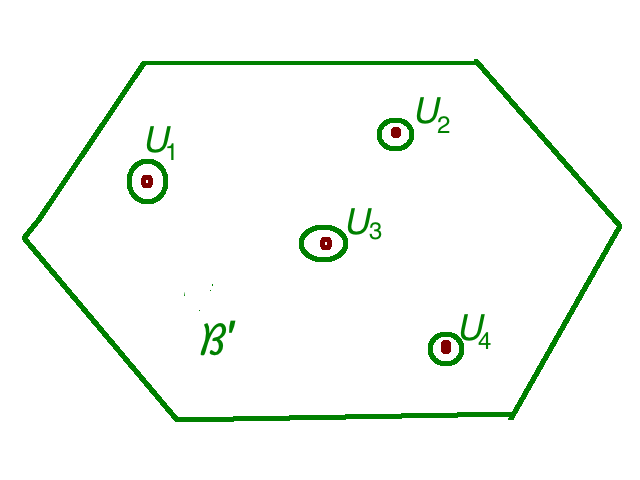
\includegraphics[width=2.5in]{BadPoints33.png}
 \end{center}
\caption{\small $\B'$ 由从布里渊区中每个坏点 $p_\alpha$ 周围挖去小开集 $U_\alpha$ 而定义。\figloc{7}{10}}
 \label{badt}
\end{figure}

% [Tutor Note: 易错——斯托克斯定理的符号依赖定向：$\partial\B'=\cup_\alpha S_\alpha$ 取相对 $\B'$ 的外法向，而 $S_\alpha$ 的定向须与式 (\ref{wn}) 中 $\epsilon^{\mu\nu}$ 所对应的 $p$ 空间定向一致，下文和式前的正号才成立。另该步的积分域写作 $B'$，与上下文的 $\B'$ 记号不统一（原文如此）。]
对每个坏点 $p_\alpha$，令 $U_\alpha$ 是围绕 $p_\alpha$ 的小开球，其边界为球面 $S_\alpha$。
令 $\B$ 为完整的布里渊区，$\B'$ 为从 $\B$ 中挖去所有 $U_\alpha$ 后所得的区域。
于是 $\B'$ 的边界为 $\partial \B'=\cup_\alpha S_\alpha$（图~\ref{badt}）。
于是由斯托克斯定理，
\begin{align}\notag 0&=\frac{1}{4\pi}\int_{B'}\d^3p\,\, \partial_\lambda\left(\epsilon^{\lambda\mu\nu} (n\cdot  
\partial_\mu n\times\partial_\nu n)\right)\cr &=\sum_\alpha\frac{1}{4\pi}\int_{S_\alpha}\d^2 p\,\,\epsilon^{\mu\nu} \,\,
\vec n\cdot \partial_\mu \vec n\times \partial_\nu \vec n \cr &=\sum_\alpha w(S_\alpha).\end{align}
因此，各坏点处缠绕数之和为零，如所承诺。

用微分形式的语言，可以把这一论证更简短地表述如下。令 $\eta$ 是 $S_{\vec n}$ 的体积形式。
于是 $\eta$ 是一个闭 2-形式，其积分为 1：
\be\label{weta}0=\d \eta,~~~\int_{S_{\vec n}}\eta = 1.\ee
给定映射 $\varphi:S\to S_{\vec n}$，相应的缠绕数为
\be\label{wnn} w(S)=\int_S\varphi^*(\eta).\ee
于是
\be\label{cl}0=\int_{B'}\varphi^*(\d \eta)=\int_{B'}\d \varphi^*(\eta)=\sum_\alpha\int_{S_\alpha}\varphi^*(\eta)=\sum_\alpha w(S_\alpha).\ee

\subsection{贝里联络}

% [Tutor Note: 术语——本节首次出现贝里联络（Berry connection）、线丛（line bundle）、平行移动（parallel transport）、曲率（curvature）与和乐（holonomy）。作者强调“更根本地”是线丛本身：联络是线丛上的附加结构，而第一陈类只依赖线丛的同构类。]
对同一结果的另一种处理方式涉及{\it 贝里联络}，更根本地，涉及使贝里联络成为联络的
那个线丛。这种处理方式在推广中有用。
对每个远离坏点的 $p$，哈密顿量 $H(p)$ 有一个负本征值，因此动量为 $p$ 的填充费米子态
构成一个一维复向量空间，我把它记作 $\L_p$。描述这一情形的漂亮说法是：随着 $p$ 变化，
$\L_p$ 作为布里渊区 $\B$ 上复线丛 $\L$ 的纤维而变化。$\L_p$ 中的向量是满足
$H(p)\psi_p=-\psi_p$ 的波函数 $\psi_p$。我们可以要求 $\psi_p$ 归一化，
$\langle\psi_p,\psi_p\rangle=1$，但没有自然的方式固定 $\psi_p$ 的{\it 相位}。

\begin{figure}
 \begin{center}
   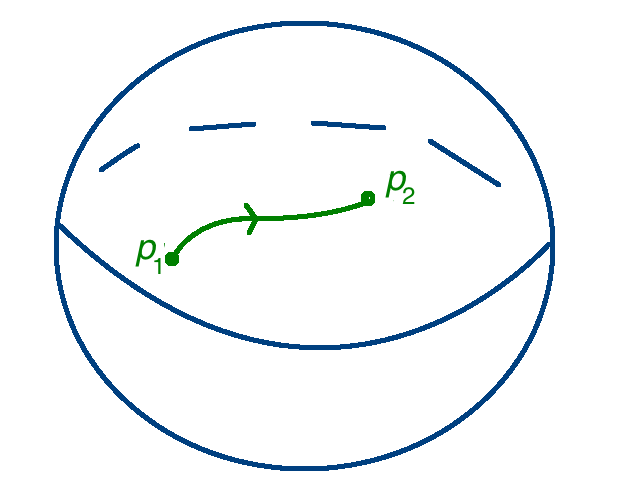
\includegraphics[width=2.5in]{Berry.png}
 \end{center}
\caption{\small 在某个参数空间中的一条路径上输运量子波函数。可以把该参数空间想象为
一个包围布里渊区中某个坏点的球面。\figloc{8}{11}}
 \label{berry}
\end{figure}

然而，假定我们沿一条路径 $p=p(s)$ 连续地改变 $p$，比如从 $p_1$ 到 $p_2$，
如图~\ref{berry} 所示。例如，可以考虑位于某个坏点 $p_*$ 周围球面
$|p-p_*|=\epsilon$ 内的路径。若我们在 $p=p_1$ 处对 $\psi_p$ 的相位作任意选择，
就可以沿给定路径平行移动 $\psi_p$ 的相位，其要求是沿路径的所有 $p$ 处都有
\be\label{zb}\langle \psi_p,\frac{\d}{\d s}\psi_p\rangle = 0. \ee
具体地说，该方程的实部保证 $\langle \psi_p,\psi_p\rangle$ 沿路径为常数，
而虚部决定 $\psi_p$ 的相位如何依赖于参数 $s$。

% [Tutor Note: 含糊——“modulo torsion”指 de Rham 上同调 $H^2(\B';\RR)$ 只能看到第一陈类 $c_1(\L)\in H^2(\B';\Z)$ 的自由部分；曲率积分给出的是 $c_1$ 在实系数下的像，挠部分在实系数下不可见。复线丛的 $c_1$ 一般可以含挠（例如透镜空间上的平坦线丛），只是本文的 $\B'$（三维环面挖去小球）的 $H^2$ 无挠，这一限定在此自动成立。]
有一条沿任意路径平行移动 $\psi_p$ 相位的法则，就等于在 $\B'$ 上（更确切地说，
在我们正平行移动其截面的线丛 $\L\to \B'$ 上）定义了一个{\it 联络}。
复线丛 $\L$ 上的一个{\it 联络}等同于一个阿贝尔规范场，我们把它记作 $\A$。
用贝里联络沿闭合圈 $\gamma$ 作平行移动，并不会把我们带回起点（图~\ref{closedberry}）。
也就是说，贝里联络不是平坦的；它有曲率 $\F=\d \A$。这个曲率除以 $2\pi$，
表示（模去挠部分）线丛 $\L\to \B'$ 的{\it 第一陈类}：
\be\label{fc}c_1(\L)\longleftrightarrow \frac{\F}{2\pi}.\ee

\begin{figure}
 \begin{center}
   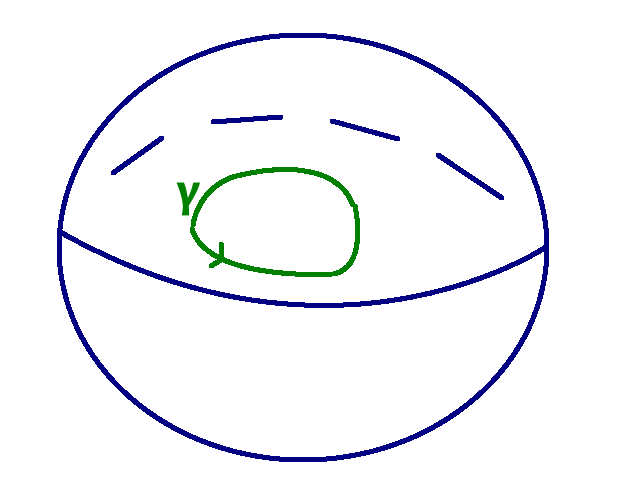
\includegraphics[width=2.5in]{ClosedLoop.png}
 \end{center}
\caption{\small 波函数沿闭合圈的平行移动。\figloc{9}{12}}
 \label{closedberry}
\end{figure}

% [Tutor Note: 易错——式 (\ref{zif}) 把 $\F/2\pi$ 在 $S_\alpha$ 上的通量等同于缠绕数，依赖 $\F/2\pi$ 是 $c_1(\L)$ 的曲率代表、且 $S_\alpha$ 与坏点周围的小球面同伦等价。式 (\ref{wif}) 的比安基恒等式对任意阿贝尔场自动成立（因 $\F=\d\A$），这正是尼尔森-二宫定理的第二个证明与第一个（斯托克斯）本质相同的原因。]
若 $p_\alpha$ 是两条能带相交的某个坏点、$S_\alpha$ 是围绕 $p_\alpha$ 的小球面，
则 $\F/2\pi$ 在球面 $S_\alpha$ 上的通量就是前面定义的缠绕数：
\be\label{zif}w_\alpha(S)=\int_{S_\alpha}\frac{\F}{2\pi}.\ee
任何阿贝尔规范场 $\A$ 的比安基恒等式断言
\be\label{wif}\d\F=0.\ee
于是我们又一次得到尼尔森-二宫定理
\be\label{nna}0=\int_{B'}\frac{\d \F}{2\pi}=\sum_\alpha\int_{S_\alpha}\frac{\F}{2\pi}=\sum_\alpha w(S_\alpha).\ee

于是，一般两带系统中布里渊区内坏点的更精确图景如图~\ref{twoob} 所示。
标以 $+$ 或 $-$ 的坏点承载正手征性或负手征性的无能隙外尔费米子；尼尔森-二宫定理
表明 $+$ 点与 $-$ 点一样多。
\begin{figure}
 \begin{center}
   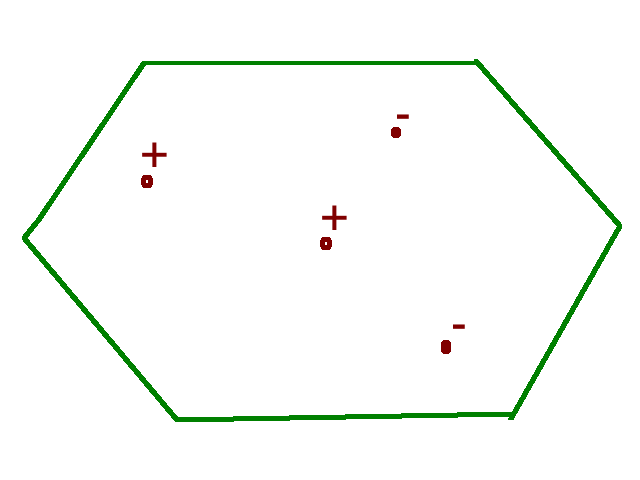
\includegraphics[width=2.5in]{BadPoints2.png}
 \end{center}
\caption{\small 一般地，布里渊区中的能带交叉点承载正手征性与负手征性的外尔费米子。
尼尔森-二宫定理表明两种类型一样多，如图所示。\figloc{10}{13}}
 \label{twoob}
\end{figure}

% ======================================================================
%  第一讲（续）　1.5-1.8 节
% ======================================================================
\subsection{一些例子}\label{somex}

% [Tutor Note: 易错——这里对比两种“湮灭”机制：相对论性的四分量狄拉克费米子可以加裸质量项，使四个分量两两配对而打开能隙；两带系统则写不出与 $\vec b\cdot\vec\sigma$ 相容的常数质量项（$\sigma_3$ 项已被吸收进 $\vec b$），只能靠 $f(p_3)$ 的零点随参数移动、并合而湮灭。这正是后文式 (\ref{terf})、(\ref{werf}) 的模型所展示的。]
具体看看两个相反手征性的坏点如何随参数变化而湮灭，是有启发性的。在相对论物理中，
这可以如下发生（这里稍稍超前一点，因为我们尚未对多于两条能带的系统陈述
尼尔森-二宫定理）。考虑一个四带系统，其中前两条能带描述一个正手征性的外尔费米子，
后两条能带描述一个负手征性的外尔费米子。这四条能带合起来描述一个四分量狄拉克费米子。
狄拉克费米子可以有裸质量；当我们向哈密顿量加入裸质量项时，能带交叉便消失了。

% [Tutor Note: 易错——式 (\ref{terf}) 中 $\vec b=(p_1,p_2,f(p_3))$，故式 (\ref{perd}) 的 $\det(\partial b_i/\partial p_j)=f'(p_3)$：零点处的手征性由 $f'$ 的符号给出。原文“depending on the sign of $\d f/\d p_3$”与之一致；核对时注意 $\vec b$ 的分量次序，即 $\sigma_3$ 位于第三分量。]
% [Tutor Note: 含糊——“a pair of Weyl points with positive or negative chirality at $p_3=\pm\sqrt a$”应读作“在 $p_3=+\sqrt a$ 与 $p_3=-\sqrt a$ 处分别有一个正、一个负手征性的外尔点”：$\d f/\d p_3=2p_3$ 在两个零点处符号相反。若按字面读成“两个点同为某种手征性”，则与 1.3 节的尼尔森-二宫定理矛盾。]
这是通常的相对论图景；但在凝聚态物理中自由更多，两个坏点的湮灭完全可以发生在
两带系统中。考虑显式哈密顿量
\be\label{terf}H(p_1,p_2,p_3)=\begin{pmatrix} f(p_3) & p_1-\i p_2\cr p_1+\i p_2 & -f(p_3)\end{pmatrix}.\ee
若 $f(p_3)=p_3$，这就是外尔费米子的基本哈密顿量 $H=\vec\sigma\cdot \vec p$。更一般地，
若 $f(p_3)$ 是任何只有单零点的光滑函数，则能带交叉出现在 $f(p_3)$ 的任一零点处
（此时 $p_1=p_2=0$），并根据该零点处 $\d f/\d p_3$ 的符号给出正手征性或负手征性的
外尔费米子。一个简单模型
\be\label{werf}f(p_3)=p_3^2-a \ee
在 $a>0$ 时于 $p_3=\pm\sqrt a$ 给出一对正、负手征性的外尔点。两个外尔点在 $a=0$ 时
并合，在 $a<0$ 时消失。这一现象在两带系统的相对论物理中不会出现，因为
$\vec p=a=0$ 附近的有效哈密顿量既没有洛伦兹对称性，甚至也没有旋转对称性。

% [Tutor Note: 笔误——本小节首句原文作“If is also of some interest...”，句首 If 疑应为 It；又上段末“near $\vec p=a=0$”中 $a$ 是标量参数，与矢量 $\vec p$ 并列不合法，应读作“$\vec p=0$ 且 $a=0$”。]
% [Tutor Note: 含糊——原文称该有效哈密顿量“甚至没有旋转对称性”，宜理解为“没有完整的 $SO(3)$ 旋转对称性”：$f(p_3)=p_3^2-a$ 仍保持绕 $p_3$ 轴的 $SO(2)$，并在 $f$ 为偶函数时保持 $p_3\to-p_3$ 的反射——正是这一反射把两个手征相反的外尔点配成对。]
% [Tutor Note: 易错——式 (\ref{teref}) 中 $g$ 的零点阶数即坏点的缠绕数：$g(x)=x^s$ 时映射 $x\mapsto x^s$ 的度为 $s$，故“多重性 $s$”与 $|w|=s$ 是同一件事，它在一般微扰下分裂为 $s$ 个缠绕数为 $+1$ 的点。注意该模型的全部坏点缠绕数之和为 $s\neq0$，因为 $\vec b$ 在大 $|p|$ 处不闭合、它不是紧致布里渊区上的合法能带哈密顿量；尼尔森-二宫定理的适用前提在此并不满足。]
看看多重性 $s>1$ 的能带交叉点如何分裂成 $s$ 个多重性为 1 的点，也颇有意义。
为此，考虑模型哈密顿量
\be\label{teref}H(p_1,p_2,p_3)=\bp p_3 & \bar {g(x)}\,\cr g(x) & -p_3\ep,\ee
其中 $g$ 是复变量 $x= p_1+\i p_2.$ 的多项式。若 $g(x)=x$，我们又回到基本的外尔
哈密顿量。能带交叉出现在 $g$ 的零点处（此时 $p_3=0$）。单零点给出正手征性的外尔点，
多重零点给出更高多重性的能带交叉点。于是例如，取
$g(x)=\prod_{i=1}^s(x-b_i)$：若所有 $b_i$ 相等，则得到只含一个多重性为 $s$ 的能带
交叉点的模型；若 $b_i$ 是一般的，则得到 $s$ 个各具多重性 1 的这样的点。

\subsection{费米能处的能带交叉}\label{bce}

迄今为止，我们已经看到由手征狄拉克哈密顿量描述的能带交叉如何能在凝聚态物理中
自然地出现。但若要它有引人注目的后果，把能带交叉放在随便一个能量上是不行的；
我们真正关心的只是位于或非常接近费米能 $\veps_F$ 的能带交叉。因此我们希望图景像
图~\ref{choices} 中右边那样，而不是左边那样。此外，若能带结构在布里渊区的一部分
如图中右边所示、在另一部分如图中左边所示，那也是不行的。在那种情况下，我们会得到
一个“普通金属”（因为那个位于 $\veps_F$ 之上或之下的能带交叉），而它的效应大概会
淹没由位于 $\veps_F$ 的能带交叉所带来的更微妙的“半金属”效应。

% [Tutor Note: 术语——图 \ref{choices} 的图注把“低于/恰好位于费米面”与正文的“低于/位于 $\veps_F$”混用。费米面是动量空间中的曲面，能带交叉的“高低”严格说应相对费米能而言；译文照原文措辞作“费米面”，读者按“费米能”理解即可。]
\begin{figure}
 \begin{center}
   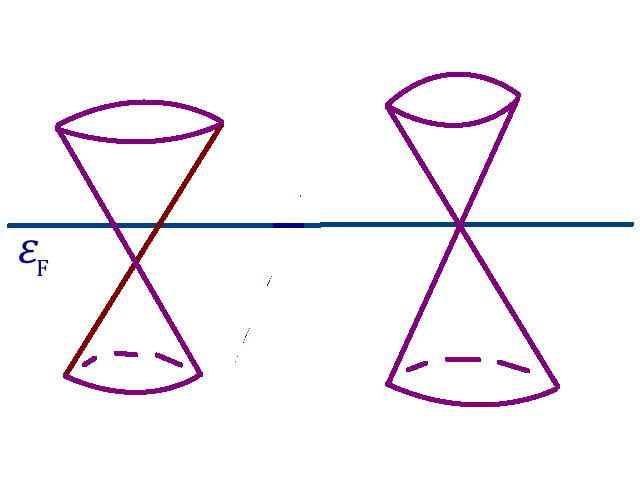
\includegraphics[width=2.5in]{GoodBad.png}
 \end{center}
\caption{\small 能带交叉位于费米面下方（左）或位于费米面上（右）。\figloc{11}{14}}
 \label{choices}
\end{figure}

理想情形下，我们希望费米面只由有限个外尔点组成，在这些点上两条能带恰好在
$\veps_F$ 处相交。这样的点必然有偶数个，且其手征性之和为零。我们怎样才能安排得使
{\it 所有}能带交叉都发生在 $\veps_F$ 处？作为第一步，怎样安排才能使它们都位于同一
能量？在凝聚态物理的语境中，做到这一点的办法是找到这样一种材料：它具有离散的
空间对称性（和/或时间反演对称性），能把所有坏点相互置换。其中某些对称性必须是空间
或时间定向反转的，因为它们必须交换 $+$ 点与 $-$ 点。于是图景会更像图~\ref{symbands}
所示，具有一个交换两个坏点的左右对称性。
\begin{figure}
 \begin{center}
   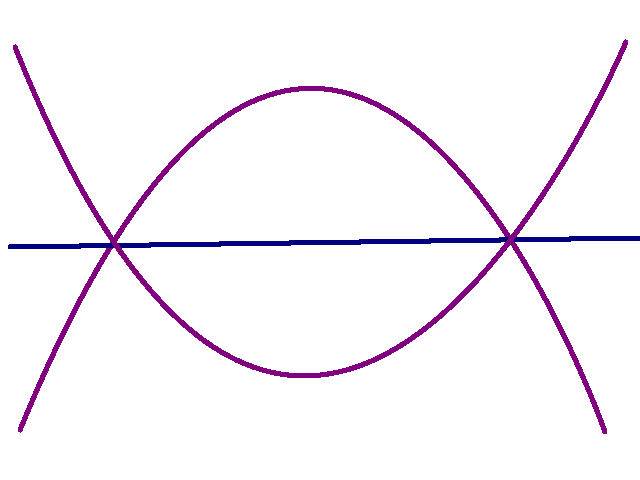
\includegraphics[width=2.5in]{SymBands.png}
 \end{center}
\caption{\small 由离散左右对称性相联系的两个能带交叉点。每原胞电子数为整数这一事实，
使两者自然都落在费米面上。\figloc{12}{15}}
 \label{symbands}
\end{figure}

% [Tutor Note: 含糊——“每原胞电子数为整数”之所以使交叉落在 $\veps_F$，实质是整数填充论证：两条能带、每原胞一个电子即半满，故费米能必落在上下两支之间；其前提是所考虑的能区内每条能带对每个 $\vec p$ 恰贡献一个态（没有额外的费米面片），否则只能保证费米能落在某条能带内部。]
但怎样才能安排得使能带交叉发生的能量恰为 $\veps_F$？这里我们遇到本主题中美好的一点。
我们可以不付代价地得到它，因为每原胞的电子数是整数。例如，若每原胞恰有一个电子应当
填充我们模型中的这两条能带，则费米能正会在我们所要的地方，因为图~\ref{symbands} 中，
在远离两个坏点的每一个动量 $\vec p$ 处，恰好有一个态位于 $\veps_F$ 之下、一个态位于
$\veps_F$ 之上。因此在半满时，能带交叉的能量就是费米能。
这一现象有许多重要的例子。最古老、最著名的是石墨烯（在二维中），我们将在第三讲中
讨论。较新的例子涉及三维中的外尔半金属。

% [Tutor Note: 术语——“universality class”在此不是统计物理意义上的“普适类”，而指“由对称性所决定的能带结构的稳健行为”。原文强调的是：能带交叉恰在 $\veps_F$ 并非拓扑强制，只是对称性下的自然（generic）结果，足够大的保对称形变会把它推开。]
更确切地说，在这种情况下能带交叉位于 $\veps_F$ 是自然的，其含义是：给定一个我们所
假设的那种能带哈密顿量，任何具有相同对称性的邻近能带哈密顿量都在定性上导致
图~\ref{symbands} 的图景。但这一结果并不被普适类所强制；只要保持离散对称性的形变
足够大，就会给出一个普通金属。我们在图~\ref{symbands3} 中展示了如何在保持其对称性的
同时修改能带结构，使能级交叉不再位于费米能处。
\begin{figure}
 \begin{center}
   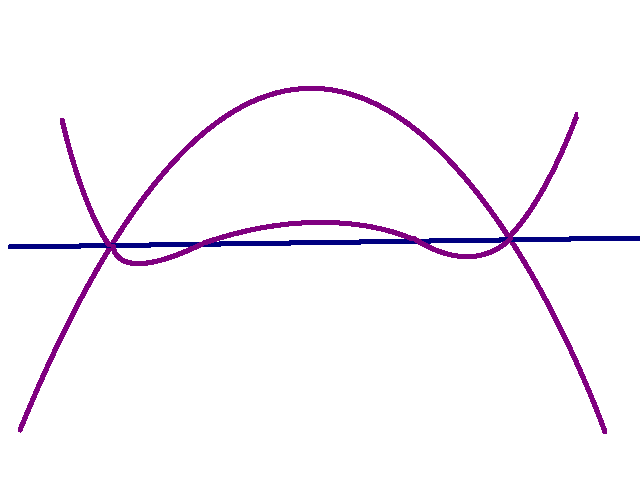
\includegraphics[width=2.5in]{SymBands3.png}
 \end{center}
\caption{\small 这一能带结构与图~\ref{symbands} 具有相同的左右对称性，但描述的是
普通金属而非外尔半金属。原因在于：在此能带结构中，能带交叉的能量（由水平线标出）
低于下能带中的某些态，因而低于费米能。\figloc{13}{16}}
 \label{symbands3}
\end{figure}

\subsection{包含自旋}

琢磨“若每原胞恰有一个电子填充这两条能带，则能带交叉将发生在 $\veps_F$”
这一说法时，人们或许会问：这一计数是否已经包含自旋？事实上，我们的讨论一直如此
一般，以至于无论是否包含自旋都成立。不过，有两种略有不同的情形。

% [Tutor Note: 易错——自旋加倍后每个外尔点变成两个同手征的外尔费米子，故“2 chiral Weyl fermions”意味着手征性计数要乘 2。类似的 $2\times$ 因子在第三讲霍尔丹模型中给出量子霍尔系数 $2\times(1/2+1/2)=2$；它与陈-西蒙斯系数的整性无关，也不影响 Nielsen-Ninomiya 的成对结论。]
一种情形是自旋-轨道耦合重要。此时把自旋看成与轨道运动退耦不是一个好近似。
我们一直在画的能带是精确能带，已经把自旋及自旋相关力考虑在内。第二种情形是自旋
相关力很小，起初忽略它们而只考虑轨道运动。在这种情形下，由狄拉克哈密顿量描述的两条
能带是轨道能带。把自旋纳入后，在一级近似下我们只是把图景加倍，于是现在有四条能带——
熟悉图景的两份拷贝。在此近似下，我们得到 2 个手征外尔费米子，且它们具有相同的手征性，
因为（若自旋与轨道运动退耦）自旋向上与自旋向下的电子具有相同的能带哈密顿量，
从而具有相同的手征性。

然而，自然界中总有自旋-轨道力，一般地两对能带会发生劈裂。精确问题是四带问题。
假定电子密度使得 4 条能带中有 2 条应当被填充，则我们所关心的交叉（因为它们可能位于
或非常接近费米能）是第二与第三能带之间的交叉（按能量递增排序）。我们马上要讲到的
尼尔森-二宫定理的 $N$ 带版本保证：第二与第三能带之间仍会有两个外尔交叉（手征性与
之前相同），但一般地处于略微不同的能量与动量。费米能不可能等于这些交叉中每一个的
能量；一般地它不等于其中任何一个，但假定自旋-轨道力很弱，它会与之接近。

\begin{figure}
 \begin{center}
   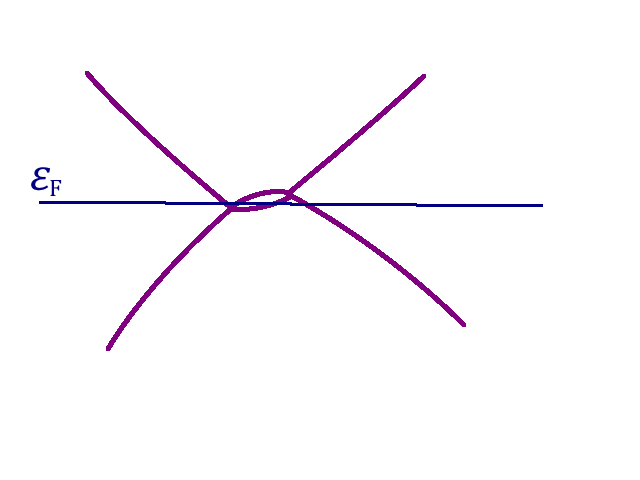
\includegraphics[width=3.5in]{Crude.png}
 \end{center}
\caption{\small 两个彼此靠近、但并不正好位于费米能处的能带交叉。\figloc{14}{17}}
 \label{crude}
\end{figure}

两个彼此靠近、但两者都不正好位于费米能处的外尔交叉，其很粗糙的图景见图~\ref{crude}。
朴素地看，这导致载流子密度极小的普通金属；但这不是全部，因为载流子密度极小时
费米液体理论并不怎么适用。

\subsection{多能带系统}

现在让我们讨论尼尔森-二宫定理对 $N$ 带系统的推广。我们假定电子密度使得应当有 $k$ 条
能带被填充，其中 $k<N$ 为某整数。令 $\H_p$ 为动量 $p$ 处完整的 $N$ 维态空间。
在任何使第 $k^{th}$ 条能带（按能量递增排序）不与第 $k+1^{th}$ 条相交的 $p$ 值处，
$\H_p$ 有一个由最低的 $k$ 个态张成的确定子空间 $\H'_p$。在第 $k^{th}$ 条能带与
第 $k+1^{th}$ 条能带相遇的点处，$\H'_p$ 的定义没有意义。与从前一样，要使这种情况
发生必须调节三个参数，因此如同图~\ref{badp} 那样，布里渊区中将有有限多个坏点，
在那里 $\H'_p$ 没有定义。

% [Tutor Note: 易错——式 (\ref{npn}) 的证明中：$\pi_2(\Gr(k,N))\cong\Z$ 给出缠绕数的整性；贝里联络是 $U(k)$ 规范场，曲率为 $\F=\d\A+\A\wedge\A$，只有 $\Tr\F$（而非 $\F$ 本身）由比安基恒等式保证为闭，故第一陈类取 $\Tr\F/2\pi$，$w(S_\alpha)$ 即 $\H'$ 在 $S_\alpha$ 上的第一陈数。]
凡 $\H'_p$ 有定义之处，它都定义了 $\H_p\cong \C^N$ 的一个 $k$ 维子空间。$\C^N$ 的
所有 $k$ 维子空间构成的空间称为格拉斯曼流形 $\Gr(k,N)$。若 $p_\alpha$ 是 $\H'_p$
没有定义的孤立点，则 $\H'_p$ 在围绕 $p_\alpha$ 的小球面 $S_\alpha$ 上有定义。
因为
$\pi_2(\Gr(k,N))\cong \Z,$
我们可以给每个 $p_\alpha$ 附上一个整数值的缠绕数 $w(S_\alpha)$。

我们先前为两带情形给出的任何一种解释都可稍加改造，用以证明尼尔森-二宫定理
\begin{equation}\label{npn}\sum_\alpha w_\alpha=0.\end{equation}
例如，让我们考虑基于贝里联络的解释。如从前一样，令 $\B'$ 为挖去坏点的小邻域后
布里渊区的“好部分”，则我们有一个秩 $k$ 的复向量丛 $\H'\to 
\B'$，其在 $p\in 
\B'$ 处的纤维为 $\H'_p$。
这正是由最低的 $k$ 条能带张成的丛。该丛上有一个贝里联络，现在它是一个 $U(k)$
规范场。

% [Tutor Note: 含糊——脚注指出的自由度：$\psi_p(s)\in\H'_{p(s)}$ 只把 $\psi_p(s)$ 确定到“可加上 $\H'_{p(s)}$ 中任意元素”的程度；式 (\ref{zomo}) 用“$\d\psi/\d s$ 与 $\H'_p$ 正交”把这一自由度固定，这正是 $\H'$ 上联络的水平条件。]
它的定义如下。为把 $\psi_p\in \H'_p$ 沿路径 $\gamma \subset B'$ 平行移动
（图~\ref{berry}），我们要求\footnote{$\psi_p(s)$ 对所有 $s$ 都应属于 $\H'_{p(s)}$，
这一条件把 $\psi_p(s)$ 对 $s$ 的依赖确定到可以加上一个依赖于 $s$ 的 $\H'_{p(s)}$
元素的程度。这一自由度由式 (\ref{zomo}) 固定。}
\be\label{zomo}\langle \psi'|\frac{\d}{\d s}|\psi\rangle=0,~~~{\mathrm{for~all}}~~\psi'\in\H'_p.\ee 
换言之，要求 $\d\psi/\d s$ 对所有 $s$ 都与 $\H'_p$ 正交。这在 $\H'\to B'$ 上给出
一个联络或 $U(k)$ 规范场 $\A$。它有曲率 $\F=\d\A+\A\wedge \A$。缠绕数
$w(S_\alpha)$ 为
$$w(S_\alpha)=\int_{S_\alpha}c_1(\H')=\int_{S_\alpha} \,\frac{\Tr\, \F}{2\pi}.$$  

利用比安基恒等式 $\d\Tr\,\F=0$，并借助斯托克斯定理，我们得到
\be\label{mpf}0=\int_{B'}\d\frac{\Tr\,\F}{2\pi}=\sum_\alpha\int_{S_\alpha} \frac{\Tr\,\F}{2\pi}=\sum_\alpha w(S_\alpha).\ee
因此，基于贝里联络的证明与两带情形相同，只不过处处都要加上一个迹。

一般地，坏点处的缠绕数为 $\pm 1$，与两带情形一样。缠绕数为 $\pm 1$ 的交叉处的
一般行为，就是第 $k^{th}$ 条与第 $k+1^{th}$ 条能带之间熟悉的外尔交叉
（图~\ref{generi}）。因此缠绕数为 $\pm 1$ 的点给出手征外尔费米子；尼尔森-二宫定理
指出，正手征性与负手征性的这类点一样多。

\begin{figure}
 \begin{center}
   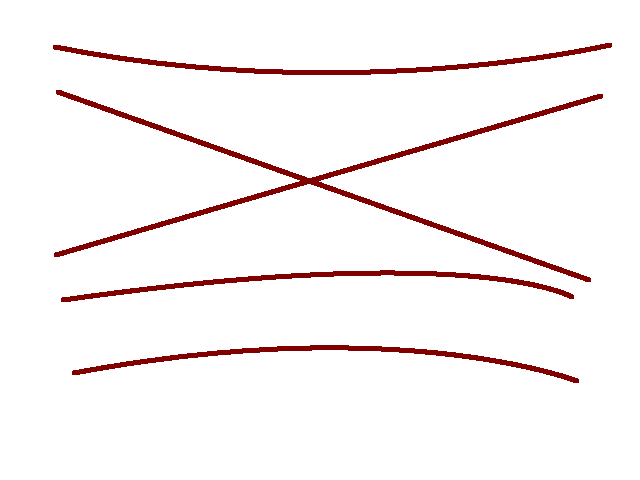
\includegraphics[width=2.5in]{Generic.png}
 \end{center} 
\caption{\small 对任意 $k$，第 $k^{th}$ 条能带与第 $k+1^{th}$ 条能带之间的一般交叉，
都由我们最初在两带系统情形中遇到的那个手征狄拉克哈密顿量支配。\figloc{15}{18}}
 \label{generi}
\end{figure}

\subsection{二维}\label{td}

以上讨论都不依赖离散对称性；不过若确实考虑具有离散对称性的材料，其中许多内容会变得更丰富。
但如果我们想在 2 维空间（而非 3 维）中得到无质量狄拉克费米子，又当如何？
不借助离散对称性，这是做不到的：因为在 2 维布里渊区中随 2 个参数变化时，一般不会有能带交叉。

% [Tutor Note: 易错——$2+1$ 维中三个泡利矩阵同时充当 $\gamma$ 矩阵（在号差 $(-,+,+)$ 下可取
% $\g^0=\i\sigma_3$、$\g^1=\sigma_1$、$\g^2=\sigma_2$ 之类的约定），故二分量旋量即可，
% 这与 $3+1$ 维必须用 $4\times4$ 矩阵、四分量旋量不同。另请注意 $\pm|p|$ 交叉之所以非普遍：
% 两带模型的能级简并要求 $b_1=b_2=b_3=0$ 三个实条件，而 2 维布里渊区只有 2 个参数；
% 只有对称性迫使 $b_3\equiv0$ 时，能带交叉才由调节 $p_1,p_2$ 保证（对照 1.2 节"三维"中
% "3 个条件、3 个参数"的讨论，以及本节式 (\ref{twod}) 与式 (\ref{hamt})）。]
在 $2+1$ 维中，只有三个 $\gamma$ 矩阵 $\gamma^0,\gamma^1,\gamma^2$，它们可以取 2 维表示。因此
$2+1$ 维的狄拉克费米子只有 2 个分量，其无质量狄拉克哈密顿量为
\be\label{twod}H=\sigma_1 p_1+\sigma_2 p_2.\ee    （要由相对论狄拉克方程 $\gamma^\mu\partial_\mu\psi=0$ 导出此式，
基本上是仿照 3 维空间中式 (\ref{hameq}) 的推导。）
我们能级为 $\pm |p|$，在 $p=0$ 处有能级交叉。我们知道，这样的能级交叉在 2 维空间中是非一般的；
具体地说，可以给狄拉克哈密顿量加一个质量项来微扰它：
\be\label{hamt}H=\sigma_1 p_1+\sigma_2 p_2+\sigma_3 m.\ee
有质量的狄拉克哈密顿量具有非简并能级 $\pm\sqrt{p^2+m^2}$。

% [Tutor Note: 易错——式 (\ref{zono}) 的 $\sR=\sigma_2$ 与式 (\ref{zamt}) 的 $\sT=\pm\sigma_1$
% （配合复共轭）都依赖"$\sigma_i$ 取实泡利矩阵"这一表示。核验时注意 $\sT$ 是反幺正的
% （$\sT\i=-\i\sT$），且 $x_1\to-x_1$ 使 $p_1\to-p_1$：$\sR$ 与 $\sT$ 都把质量项 $m\sigma_3$
% 变为 $-m\sigma_3$，故它在这两种变换下均为奇。式 (\ref{zamt}) 的 $\pm$ 号不可丢——它对应
% 把复狄拉克场分解为两个马约拉纳场时二者在 $\sT$ 下的相对符号（见紧随本段的脚注），
% 也正是拓扑超导体中区分不同相的关键（正文末句已提及）。]
然而，质量项破坏了一些对称性。$H=\sigma_1 p_1+\sigma_2 p_2$
的{\it 反射}对称性为
\be\label{zono}\sR\psi(t,x_1,x_2)= \sigma_2\psi(t,-x_1,x_2)\ee
而质量项
\be\label{ozono}H'=m\sigma_3\ee
在它之下为奇。质量项在时间反演下同样为奇。对于哈密顿量 (\ref{hamt}) 以及
$\sigma$ 矩阵的标准表示\footnote{在研究具有 $\sT$ 不变性的理论时，通常更方便的是从实的
$2\times 2$ 伽马矩阵 $\g_\mu$ 出发，我们一般都这样做。此时哈密顿量中出现的 $\sigma$ 矩阵就是实矩阵
$\sigma_i=\g_0\g_i$，如式 (\ref{sigmam}) 所示。在这样的约定下，$\sT$ 的作用为
$\sT\psi(t,\vec x)=\pm\g^0\psi(-t,\vec x)$。这里隐含了如下事实：设把复（狄拉克）费米子场 $\psi$
用两个厄米（马约拉纳）费米子场 $\chi_1,\chi_2$ 展开，即 $\psi=\chi_1+\i\chi_2$；那么 $\chi_1$ 与 $\chi_2 $
在 $\sT$ 下以相反的符号变换：$\sT\chi_1(t,\vec x)=\pm \g^0\chi_1(-t,\vec x)$、
$\sT\chi_2(t,\vec x)=\mp \g^0\chi_2(-t,\vec x)$。由于 $\sT$ 是反幺正的，$\sT\i=-\i\sT$，
正是 $\chi_1$ 与 $\chi_2$ 变换中的相反符号保证了我们为 $\psi$ 断言的那个简单变换。
后面（脚注 \ref{memo}）描述 3 维空间中 $\sT$ 的作用时，有类似的陈述。}，
时间反演为
\be\label{zamt}\sT\psi(t,\vec x)=\pm\sigma_1\psi(-t,\vec x). \ee
这个符号实际上具有物理意义，结果表明它在拓扑超导体理论中很重要，
不过本讲不探讨这一主题。

% [Tutor Note: 含糊——"一个分量是产生算符、一个是湮灭算符"一句是自由度计数：$2+1$ 维
% 二分量狄拉克场在给定 $\vec p$ 下只含一个正能粒子态及其反粒子态，因此对每个 $\vec p$
% 只有一个自旋态可取（$+1/2$ 或 $-1/2$ 二选一），这与 $3+1$ 维四分量旋量同时含两种自旋不同。
% 本段脚注用小群（little group）分类说明无质量粒子在 $D=3$ 时"没有自旋"：小群为
% $SO(D-2)=SO(1)$，平庸，无质量态的"自旋"只由 $SO(D-2)$ 的表示决定；而"平移"部分在所有
% 常规场论中平庸作用乃是一个动力学假设，连续自旋理论（\cite{ST}）正是放弃这一假设的尝试。]
质量项破坏反射对称性 $\sR$ 与时间反演对称性 $\sT$ 的物理原因如下。如果 $\psi$ 是 2
维中的二分量电子场，那么在任一给定的空间动量 $\vec p$ 处，$\psi$ 的一个分量是产生算符，
另一个是湮灭算符。因此对每个 $\vec p$ 值，$\psi$ 只描述一个电荷为 1 的态（以及相应的、
电荷为 $-1$ 的空穴或反粒子）。如果 $\psi$ 粒子有质量，我们就可以到它的静止系中研究它，
而它那个唯一的自旋态将在旋转群下按自旋 $1/2$ 或 $-1/2$ 变换。（在 2 维空间中，旋转群恰是
阿贝尔群 $SO(2)$，只有 1 维表示。）两种符号的选择在 $\sR$ 或 $\sT$ 下都是奇的，所以质量项
必定破坏这些对称性。相反，若 $m=0$，费米子无法被带到静止，而在 2 维空间中我们无法定义
它的自旋。\footnote{在 $D$ 维时空中，相对论性粒子的“自旋”总是由量子态在“小群”
（little group）下的变换来描述，小群是洛伦兹群 $SO(1,D-1)$ 中保持其能量-动量 $D$ 矢量
$p^\mu$ 不变的那个子群。对有质量粒子，小群是 $SO(D-1)$，自旋就是该群的一个表示。对无质量
粒子，小群是 $SO(D-2)$ 被一个非紧的“平移”群扩张所得，而“自旋”实际上由 $SO(D-2)$ 的一个
表示决定。（小群的“平移”部分在所有常规的相对论场论中都平庸地作用。关于构造一个使之不然
的理论的尝试，见 \cite{ST}。）当 $D=3$ 时，$SO(D-2)$ 是平庸的，无质量粒子的“自旋”概念
不存在。在这个说明中，我们忽略了反射与时间反演对称性。当存在离散时空对称性时，
$D=3$ 中的无质量粒子确实有确定的变换性质。} 因此 $m=0$ 的理论可以是保持 $\sR$ 与
$\sT$ 的。

这告诉我们，在 2 维晶体中，只要晶体具有适当的 $\sR$ 或 $\sT$ 对称性，就应当能够找到
无能隙的类狄拉克模；而且这些无能隙模出现在 $\sR$ 或 $\sT$ 不变的那个动量值处。举例
并不困难。最著名的例子是石墨烯；我们将在第三讲讨论这一情形。眼下我只想指出：与 3
维空间中的外尔点颇为相似，这里也有两种情形——或者是一种在计入自旋后具有 $\sR$ 或
$\sT$ 对称性、从而给出无能隙模的材料；或者是一种自旋-轨道力很小、在忽略自旋与
自旋-轨道力时具有相应性质的材料。在后一种情形中，现实世界里得到的模会有一个非常小但
并非严格为零的能隙。石墨烯中发生的正是如此 \cite{KM}。

\subsection{外尔费米子与费米弧}

现在我们开始讨论凝聚态物理中由拓扑决定的边缘模。我们将在 3 维空间中做这件事，并首先
考虑一个非手征的无质量狄拉克费米子 $\psi$。眼下先不管如何在凝聚态物理中实现它。设
$\psi$ 被限制在半空间（可能是晶体的内部），我们要问：当它从边界反射时，应当服从何种
边界条件？对于图 \ref{RightAngles} 所示的那种直角反射，一个简单的边界条件将保持
角动量守恒。

     \begin{figure}
 \begin{center}
   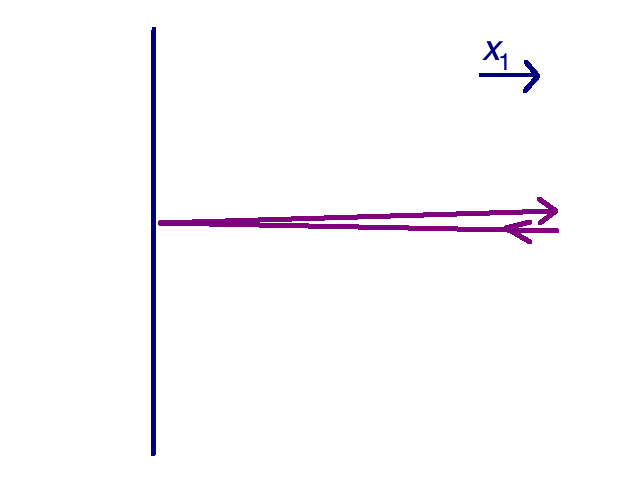
\includegraphics[width=2.5in]{RightAngles.png}
 \end{center}
\caption{\small 从边界作直角反射的粒子，若要保持其角动量，就必须反转其螺旋度
（其角动量沿运动方向的分量）。\figloc{16}{20}}
 \label{RightAngles}
\end{figure}

% [Tutor Note: 术语——螺旋度（helicity）指自旋（内禀角动量）沿动量方向的投影，
% 手征性（chirality）指 $\g_5$ 的本征值；仅对无质量费米子二者才等同（有质量时螺旋度
% 不再是好量子数）。图 \ref{RightAngles} 的图注把螺旋度说成"沿运动方向的角动量分量"与此
% 并不矛盾：因 $\vec L\cdot\vec p=0$ 恒成立，总角动量沿动量方向的分量恰等于自旋沿动量
% 方向的分量。正文随后用 $J_1$ 守恒来刻画边界条件，与此一致。]
所谓“保持角动量”，我的意思是：对于 $x_1=0$ 处的边界条件，绕 $x_1$ 轴的角动量分量
$J_1$ 应当守恒。\footnote{在晶体中，$J_1$ 可能只在模 $n$ 意义下守恒，其中 $n=2,3,4$ 或
$6$。下面的论证将表明，外尔费米子上的边界条件对任何 $n>1$ 都不能保持 $J_1$ mod $n$。}
由于散射中运动方向反转，螺旋度必须反转。对狄拉克费米子这是可能的，因为狄拉克费米子
同时具有两种螺旋度。狄拉克费米子所能具有的、保持角动量但破坏螺旋度的边界条件，
见下文式 (\ref{molof})。

 但是，对于只有一个螺旋度的无质量外尔费米子，我们能有什么样的边界条件呢？显然，边界
条件无法反转螺旋度，因而不能保持角动量守恒。任何边界条件都不得不在边界平面内挑出一个
优先方向。对于手征狄拉克哈密顿量
 \be\label{chid}H=-i\vec\sigma\cdot \frac{\partial}{\partial\vec x},\ee
 $x_1=0$ 处的一个好边界条件是
 \be\label{goodbc}\left.M\psi\right|_{x_1=0}=\left.\psi\right|_{x_1=0}\ee 其中
 \be\label{mis}M=\sigma_2 \cos\alpha+\sigma_3\sin\alpha\ee
 对某个角度 $\alpha$。

% [Tutor Note: 易错——式 (\ref{goodbc}) 的边界条件要求 $M$ 厄米、且与 $\sigma_1$ 反交换，
% 这样分部积分产生的边界项 $\langle\psi_1|\sigma_1|\psi_2\rangle\big|_{x_1=0}$ 才消失；
% 而 $\{M,\sigma_1\}=0$ 迫使 $M$ 落在 $\sigma_2$-$\sigma_3$ 平面内，归一化后即式
% (\ref{mis})。若取 $M=\sigma_1$，则 $M$ 与 $\sigma_1$ 对易而非反交换，边界项不消失，
% $H$ 不厄米。这正是该边界条件（乃至任何保持 $J_1$ mod $n$ 的边界条件）无法保持
% $x_2-x_3$ 平面旋转对称性的原因，也解释了为何外尔费米子的边界条件必须挑出一个方向 $\alpha$。]
这个边界条件之所以好，是因为它使 $H=-i\vec\sigma\cdot\vec\nabla$ 成为厄米的。要证明
$H=-i\vec\sigma\cdot\vec\nabla$ 是厄米的，即
\be\label{zeff}\langle\psi_1,H\psi_2\rangle=\langle H\psi_1,\psi_2\rangle,\ee
就必须分部积分。分部积分中可能出现的边界项会消失，因为
$\{M,\sigma_1\}=0$，
而我们选取 $M=\sigma_2 \cos\alpha+\sigma_3\sin\alpha$ 正是为了保证这一点。特别地，若取
$M=\sigma_1$ 就不行；这再次表明，该边界条件不可能在 $x_2-x_3$ 平面的旋转下不变。它甚至
不能保持这一旋转对称性的某个非平庸离散子群，而晶体中可能正好存在这样的子群。

厄米性允许我们在边界条件中出现的算符 $M$ 上再加一些依赖于动量的项；但在低动量极限下、
即在能带交叉点附近，它迫使 $M$ 取我们所写出的形式，只是 $\alpha$ 取某个值。在连续场论
中，我们本可以把 $\alpha$ 当作自由参数。在凝聚态物理中情况其实并非如此。在一个具体的
模型中，若其体能带结构导致存在一个由手征狄拉克哈密顿量描述的能带交叉点，则求解系统
边界附近的薛定谔方程将确定 $\alpha$ 的一个有效值。不过，改变边界（例如在材料表面再添加
一层原子）一般会改变这个值。

% [Tutor Note: 笔误——式 (\ref{polk}) 与式 (\ref{molt}) 的指数符号疑误。按式 (\ref{wolt})，
% $H\psi=0$ 等价于 $(\partial_1-\i\partial_3)\psi=0$；代入 $\psi=\exp(\i k_1 x_3+k_1x_1)\psi_0$
% 得 $H\psi=-2\i k_1\sigma_1\psi_0$，仅当 $k_1=0$ 才为零，这与式 (\ref{formix}) 的局域化条件
% $k_1<0$ 矛盾。欲使解在 $x_1\geq0$ 上按 $\exp(k_1x_1)$（$k_1<0$）衰减并满足 $H\psi=0$，
% 指数应作 $\exp(-\i k_1x_3+k_1x_1)$，即该边缘模沿 $x_3$ 的动量为 $-k_1$（等价地，
% $(\partial_1-\i\partial_3)\psi=0$ 的解为 $\psi\propto\exp(\lambda x_1+\i kx_3)$，
% $\lambda=-k$，故沿 $x_3$ 的动量与衰减率反号）。正文照录原文，未作改动。]
 $\alpha$ 的取值可以被 $x_2-x_3$ 平面的一个旋转吸收，因此在分析边界条件的后果时，我们
可以只考虑 $\alpha=0$ 的特殊情形，即边界条件为 $\sigma_2\psi\vert=\psi\vert$。
用这个边界条件去解薛定谔方程，会发生非常有趣的事情。让我们设 $\sigma_2\psi=\psi$ 处处
成立（而不只是在边界上），并设 $\partial\psi/\partial x_2=0$，来试着解方程 $H\psi=0$。于是
\be\label{wolt}H\psi=-\i\left(\sigma_1\partial_1+\sigma_2\partial_2+\sigma_3\partial_3\right)\psi=-\i\sigma_1(\partial_1-i\partial_3)\psi.\ee 
（回忆 $\sigma_3=-i\sigma_1\sigma_2$，故 $\sigma_3\psi=-i\sigma_1\psi$。）因此我们可以用
\be\label{polk}\psi=\exp(\i k_1 x_3+k_1x_1)\psi_0,\ee
解出 $H\psi=0$，其中 $\psi_0$ 是一个常旋量，满足
\be\label{folt}\sigma_2\psi_0=\psi_0.\ee
此外，只要
\be\label{formix}k_1<0.\ee
这个解就是平面波可归一化的。更一般地，对任何实数 $\veps$，我们都可以用
\be\label{molt}\psi=\exp(\i\veps x_2)\exp(\i k_1 x_3+k_1x_1)\psi_0.\ee
解出 $H\psi=\veps\psi$。

% [Tutor Note: 术语——本讲对 boundary（边界：三维样品的表面）与 edge（边缘：二维样品的边）的译名分工如下：
% 故 boundary condition 译"边界条件"，edge state/edge mode 译"边缘态/边缘模"，
% edge-localized state 译"边缘局域态"。本节 $2+1$ 维的边缘局域模位于 $x_1=0$ 的边界附近，
% 沿 $x_3$ 传播；后文 1.11 节 $3+1$ 维中的"edge"实际是二维表面，但 Witten 仍沿用
% edge-localized 一词，译文从术语表统一。]
假设我们的系统支撑在半空间 $x_1\geq 0$ 中，边界在 $x_1=0$，那么只要 $k_1< 0$，这些解
就沿离开边界的方向指数衰减。它们给出了凝聚态物理中由拓扑决定的边缘局域态的最早例子。

对每一个足够接近能带交叉能量、从而使上述分析适用的能量 $\veps$，我们都找到了边缘局域
态，它们支撑在 $k_1-k_2$ 平面中的一条射线 $k_1< 0$、$k_2=\veps$ 上。在这条射线的端点
$k_1=0$ 处，边缘局域化失效，解变成平面波（动量只在 $x_2$ 方向上）。因此，它与体态
无法区分。

从凝聚态物理的观点看，给定能量的边缘局域态位于动量空间中的一条直线上，这当然不具有
普适性。我们可以给哈密顿量和边界条件加上各种各样的高阶项，这会改变边缘局域态的色散
关系，正如它会改变体态的色散关系一样。然而，我们所作的分析在 $\vec k=0$ 处的能带交叉点
附近是普遍的。这一分析表明：在任何足够接近能带交叉能量的能量处，都存在一段由边缘局域
态构成的弧，称为费米弧 \cite{WTVS}。

% [Tutor Note: 笔误——此处边界取向与前文不一致。本节前文（式 (\ref{molt}) 之后）取边界在
% $x_1=0$、垂直动量 $k_1$ 不守恒，下一段也说"当 $x_1=0$ 处存在边界时，垂直分量
% $k^\perp=k_1$ 不守恒"；但这里却写边界在 $x_3=0$，并称 $k_1,k_2$ 守恒而 $k_3$ 不守恒。
% 由上下文（费米弧的端点须与某个体平面波态在 $k_1,k_2,\veps$ 上重合）判断，疑此处
% $x_3$ 应为 $x_1$；也可能是作者改取另一晶面 $x_3=0$ 而未声明坐标轴已重选。
% 两种读法都不影响“端点与体态重合”的结论，正文照录原文。]
参数化边缘局域态的弧，只能在所讨论的态不再是边缘局域态时终止。但正如我们例子中那样，
在那一点上边缘局域态变得与某个体平面波态无法区分。当 $x_3=0$ 处存在边界时，$k_1$、
$k_2$ 与 $\veps$ 守恒，而 $k_3$ 不守恒。因此费米弧端点处的 $k_1$、$k_2$、$\veps$ 之值，
将与某个具有某一 $k_3$ 值的体平面波态的相应值重合。（一般而言——尽管在我们的简单模型中
不是如此——这个值将依赖于 $\veps$。）

一端与某个能带交叉点相关联的费米弧，必然还有另一端，而那一端将与另一个能带交叉点
相关联。让我们从尼尔森-二宫定理的角度来考察这件事。一般地我们知道，布里渊区中总有多重
外尔点，设在动量 $\vec k_\alpha$ 处，$\alpha=1,\dots,s$。当 $x_1=0$ 处存在边界时，动量的
垂直部分 $k^\perp=k_1$ 不守恒，我们应当只用 $k^\parallel=(k_2,k_3)$ 来标记外尔点。

在体中，由于动量守恒，不同 $\vec k$ 值处的无能隙模彼此不“混合”，可以分开处理。但当我们
考虑边界附近的行为时，动量的“垂直”分量 $k^\perp$ 不守恒，我们只应使用 $k^\parallel$。
于是我们把坏点投影到 2 维，如图 \ref{projection} 所示。只要外尔点的投影
$k_\alpha^\parallel$ 全部互不相同，它们就会两两由费米弧连接。

% [Tutor Note: 含糊——"投影互不相同 ⇒ 两两由费米弧相连"一句跳过了实质论证。真正起作用的是
% 边界理论的净手征性：把体布里渊区的外尔点投影到表面布里渊区后，每个投影点的缠绕数须对
% $k^\perp$ 求和；净缠绕数非零的投影点必为一段费米弧的端点，而 Nielsen-Ninomiya 定理保证
% 总缠绕数为零，故端点成对出现。仅"投影互不相同"并不足以保证配对，还须两个被连接的点
% 手征性相反（即投影处的净手征性非零）。参见 \cite{WTVS} 以及第二讲 2.10 节
% （More On Fermi Arcs）关于费米弧的再讨论。]
  \begin{figure}
 \begin{center}
   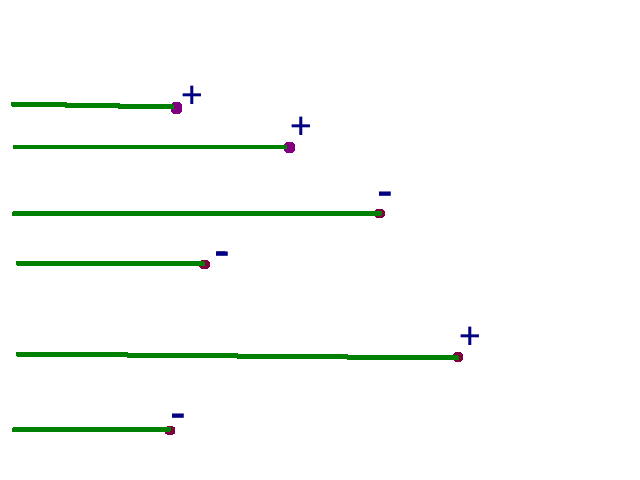
\includegraphics[width=2.5in]{Projection.png}
 \end{center}
\caption{\small 把能带交叉点从以 $\vec k$ 参数化的体布里渊区投影到只以 $k^\parallel$
参数化的表面布里渊区。（图中 $k^\perp$ 沿水平方向，$k^\parallel$ 沿竖直方向。）
一般地，能带交叉点出现在互不相同的 $k^\parallel$ 值处；此时它们的投影是费米弧的端点。\figloc{17}{23}}
 \label{projection}
\end{figure}

 但如果两个手征性相反的外尔点投影到边界动量空间的同一点，如图 \ref{special}，那么
两者都不必连接到费米弧上。从低能观点看，两个手征性相反的模合起来构成一个具有两种手征性
的狄拉克费米子。狄拉克费米子容许旋转不变的边界条件，并且可以被赋予能隙，正如我们在
\ref{df} 节所讨论的。

当然，两个给定的外尔点在投影到边界时是否重合，取决于我们考虑哪一个边界面。但使外尔点
变得有趣的离散对称性，也可能使某些晶面上两个外尔点具有相同投影这件事变得自然。事实上，
如果一个晶体具有保持平面 $x_1=0$ 的非平庸旋转群，这就必然会发生。因为单个外尔费米子
不容许任何对 $n>1$ 保持 $J_1$ mod $n$ 的边界条件，所以在存在这种守恒律时，我们绝不会
在给定的 $k^\parallel$ 处只得到一个外尔费米子。

  \begin{figure}
 \begin{center}
   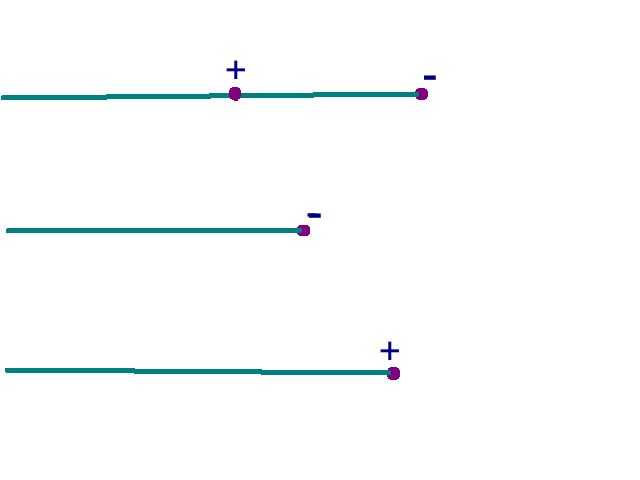
\includegraphics[width=3.5in]{Special.png}
 \end{center}
\caption{\small 离散对称性可能使两个或更多能带交叉点出现在同一个 $k^\parallel$ 值处，
这是自然的。\figloc{18}{23}}
 \label{special}
\end{figure}


\subsection{狄拉克费米子的无能隙边界模}\label{df}


由狄拉克费米子也可以得到边界局域模，这对于理解拓扑绝缘体很重要。
在没有离散对称性、也不调节任何参数的情况下，凝聚态物理中在 3 维空间里得到无质量狄拉克
（而非外尔）费米子是不自然的。对于同时具有两种手征性的四分量费米子场 $\psi$，质量项是
允许的；事实上这样的项有两个。一般的洛伦兹不变的有质量狄拉克方程为
\be\label{zolof}\left(\sum_\mu\gamma^\mu\partial_\mu -m-\i m'\gamma_5\right)\psi=0.\ee
相应的哈密顿量为
\be\label{olof}H=\g^0\vec\gamma\cdot \vec p-\i m\g^0-\i m'\g_1\g_2\g_3. \ee
 从相对论的角度看，要得到无质量狄拉克费米子，我们需要一个使 $m=m'=0$ 的理由。
自然要到对称性（时空对称性或手征对称性）中去找。

% [Tutor Note: 易错——式 (\ref{zolof})/(\ref{olof}) 的符号约定：按实伽马矩阵
% $\{\g_\mu,\g_\nu\}=2\eta_{\mu\nu}$、$\eta_{\mu\nu}=\mathrm{diag}(-1,1,1,1)$ 以及
% $\g_5=\i\g^0\g^1\g^2\g^3$，有 $\g^0\g_5=-\i\g_1\g_2\g_3$，这正是式 (\ref{olof}) 中
% $m'$ 项写成 $-\i m'\g_1\g_2\g_3$ 的来源；而 $m$ 项的符号 $-\i m\g^0$ 则依赖
% $\g_0\g_0=-1$ 与 $H=\i\partial_0$。若把 $\g_5$ 定义中的 $\i$ 换成 $-\i$（即
% $\g_5=-\i\g^0\g^1\g^2\g^3$），$m'$ 项整体变号；核对文献时务必先锁定 $\g_5$ 的约定。
% 另注意：式 (\ref{olof}) 首项写作 $\g^0\vec\gamma\cdot\vec p$，而本讲开头（式 (\ref{perf}) 之前）
% 写的是 $H=\g_0\vec\gamma\cdot\vec p$；因 $\g_0=-\g^0$，两式相差一符号，疑为原文笔误。
% 另注意两个质量项 $m,m'$ 分别破坏不同的离散对称性，故“无质量”需要两个独立的理由。]
让我们考虑假设时间反演对称性 $\sT$ 的情形。这足以把两个参数中的一个取为 0，但不能把
两个都取为 0。狄拉克方程成为\footnote{\label{memo}
此式在 $\sT\psi(t,\vec x)=\g^1\g^2\g^3\psi(-t,\vec x)$ 下不变。
我们假设伽马矩阵是实的 $4\times 4$ 矩阵，服从 $\{\g_\mu,\g_\nu\}=2\eta_{\mu\nu}$，
其中 $\eta_{\mu\nu}=\mathrm{diag}(-1,1,1,1)$。}
\be\label{lookme}\left(\sum_\mu\gamma^\mu\partial_\mu -m\right)\psi=0.\ee
 一般地 $m$ 不为 0；但当然，只要调节一个参数，我们就能使 $m$ 变为零。
  
  在凝聚态物理中，我们为使哈密顿量中某个参数变为零而调节的东西，可能例如是合金的化学
成分。然而我们注意到：虽然式 (\ref{olof}) 是这个系统的一般洛伦兹不变哈密顿量，在凝聚态
物理中我们不应假设哈密顿量具有洛伦兹不变性，因而还可能有更多的项。
更一般的哈密顿量的分析要复杂得多。但从对相对论情形的进一步研究中，我们可以得到一条
有用的教训。
  
考虑一个被限制在半空间 $x_1\geq 0$ 中的狄拉克费米子。
狄拉克算符容许一个自然的、旋转不变的边界条件
\be\label{molof}\g_1\psi|_{x_1=0}=\pm \psi|_{x_1=0},\ee
其中符号有某种选择。这与外尔费米子形成对照：如我们先前讨论过的，外尔费米子不容许旋转
对称的边界条件。边界条件 (\ref{molof}) 破坏螺旋度，因为 $\g_1$ 与手征算符（即螺旋度
算符）$\g_5=\i\g^0\g^1\g^2\g^3$ 反对易。所以它对一个外尔费米子没有意义，因为外尔费米子
是 $\g_5$ 的本征态，只有一种螺旋度。注意，边界条件 (\ref{molof}) 保持 $\sT$，其中 $\sT$
的作用如脚注 \ref{memo} 所定义，因为 $\g_1$ 与 $\g^1\g^2\g^3$ 对易。
边界条件中的符号可以通过 $\psi\to\g_5 \psi$ 反转，而这一变换同时改变式 (\ref{lookme}) 中
质量参数 $m$ 的符号。因此，只要我们同时考虑 $m$ 的两种符号，就可以在边界条件中取 $+$ 号。

% [Tutor Note: 易错——式 (\ref{molof}) 的局域化条件与质量项符号绑定：按式 (\ref{lookme})
% 质量项写作 $-m$，代入 $\psi=\exp(mx_1)\psi_\parallel$（式 (\ref{ogg})）可见，只有 $m<0$
% 时解才沿 $x_1\to+\infty$ 衰减（正文"高度不可归一化"一句即指 $m>0$）。若把质量项写成
% $+m$，或把边界条件取另一支 $\g_1\psi=-\psi$，则局域化的符号随之反转；正文随后用
% $\psi\to\g_5\psi$ 同时翻转边界条件符号与 $m$ 的符号，正是为了说明"取 $+$ 号不失一般性"。
% 另注意 $\g_1$ 与 $\g_5$ 反对易（故破坏螺旋度），却与 $\sT=\g^1\g^2\g^3$ 对易（故保持 $\sT$）。]


令 $x_\parallel $ 为沿边界的坐标，而
\be\label{zogg}\gamma\cdot\partial^\parallel=\sum_{\mu\not=1}\gamma^\mu\partial_\mu\ee
为沿边界的 $2+1$ 维狄拉克算符。
我们可以在半空间 $x_1\geq 0$ 中，用
\be\label{ogg}\psi=\exp(mx_1)\psi_\parallel(x_\parallel)\ee
满足 $3+1$ 维狄拉克方程，其中
\be\label{pogg}\gamma_1\psi_\parallel=\psi_\parallel,~~~\gamma\cdot\partial^\parallel\psi_\parallel(x_\parallel)=0.\ee
当 $m>0$ 时，这个解是高度不可归一化的。但当 $m<0$ 时，它是平面波可归一化的，并局域在
边界附近。

更确切地说，由于 $\psi_{\parallel}$ 被约束为满足无质量的 $2+1$ 维狄拉克方程
\be\label{plogg}\gamma\cdot\partial^\parallel\psi_\parallel(x_\parallel)=0,\ee
我们得到一个 $2+1$ 维无质量狄拉克费米子。（这是一个标准的 $2+1$ 维二分量狄拉克费米子，
因为原来的 $3+1$ 维四分量狄拉克费米子有一半分量被约束
$\gamma_1\psi_{\parallel}=\psi_{\parallel}$ 去掉了。）

在 $\sT$ 不变的理论中，一个体态有能隙、却具有单个边界局域无质量狄拉克费米子的相，与
一个在体和边界上都有能隙的相本质不同。这是因为，一旦我们找到单个边界局域的无质量费米子，
小的 $\sT$ 不变微扰——即使破坏洛伦兹对称性——也不会使边界产生能隙。的确，我们记得
$\sT$ 不变性不允许单个 $2+1$ 维狄拉克费米子获得质量。

% [Tutor Note: 笔误——式 (\ref{zuffo}) 的公式环境起止不匹配：原文以 \begin{equation} 起、
% 却以 \ee 结束（应为 \be 或 \end{equation}）。因 \ee 恰定义为 \end{equation}，编译无误，
% 仅为源码记号不一致，正文照录原文。另可核验：矩阵
% $-\i\bp0 &m\cr -m& 0\ep$ 确是厄米的（对角元为零、非对角元互为共轭），
% 对角化后给出 $\pm m$ 两个质量，与正文"质量等值反号"一句相符。]
  然而，$\sT$ 不变性会允许 $2+1$ 维中的{\it 一对}狄拉克费米子获得裸质量。
这样一对粒子的 $\sT$ 不变狄拉克方程为\footnote{$\sT$
的作用为 $\sT\psi_i(t,\vec x)= \g^0\psi_i(-t,\vec x)$，$i=1,2$。质量项已取为厄米的，
同时保证 $\sT$ 不变性。}
\begin{equation}\label{zuffo}\left(\sum_{\mu=0}^2\g^\mu\partial_\mu-\i  \bp0 &m\cr -m& 0\ep \right)\bp\psi_1\cr\psi_2\ep=0.\ee
（将质量项对角化后可知，这给出两个 $2+1$ 维有质量狄拉克费米子，其质量等值反号。）
因此，在一个具有 $\sT$ 不变性、没有其他特殊性质的 3 维空间凝聚态系统中，边界局域狄拉克
费米子的数目一般地要么是 0，要么是 1。这是两个不同的相；只要体理论有能隙，就不能在保持
$\sT$ 不变性的情况下从一个相变到另一个相。（当体是无能隙时，边界的无能隙模可以通过变得
与体模无法区分而消失。）
边界上存在无能隙狄拉克模的情形就是 3 维拓扑绝缘体 \cite{FMK}。
拓扑能带理论为理解这个相提供了强有力的方法，但我们不在此讨论。

% [Tutor Note: 含糊——"从普通绝缘体到拓扑绝缘体的相变一般经由中间导电相"一句，作者只引
% \cite{Mur,KK} 而未给论证。其实质是：在不假定洛伦兹不变性时，哈密顿量中除 $m,m'$ 外还有
% 其他允许的项，$m$ 过零并不直接导致能隙关闭后重开，而往往先进入无能隙的半金属相
% （外尔点或狄拉克点）；脚注 \ref{complicated} 给出了这一机制的具体版本：外尔点成对产生、
% 再重新连接并湮灭。若同时假定 $\sP$ 与 $\sT$，这一中间相可以被排除，简单模型才成立
% （见本讲 1.12 节末尾的讨论）。]
以上所述表明，当体狄拉克费米子的质量穿过 0 时，这会导致普通绝缘体与拓扑绝缘体之间的
相变。这是这两个相之间一条特别简单的路径，从相对论的观点看显得很自然。
但在凝聚态物理的语境下，只要 $\sT$ 是唯一相关的对称性，这条路径就是非一般的，因为在
凝聚态物理中哈密顿量一般还会包含不遵守洛伦兹不变性的额外项。结果表明 \cite{Mur,KK}，
一般地，从普通绝缘体到拓扑绝缘体的相变是一个更复杂的过程，中间存在一个导电相。\footnote{\label{complicated}
从一个平庸绝缘体出发，当我们改变一个参数时，系统经历 \ref{somex} 节所描述的相变，
其间出现一对相反手征性的外尔点。
这同时发生在两个等值反号的 $\vec p$ 处，二者由 $\sT$ 交换。继续变化，外尔点重新连接
并湮灭，留下一个拓扑绝缘体。} 若在 $\sT$ 之外还假定 $\sP$，那么“两类绝缘体之间的相变
涉及一个无质量狄拉克费米子”这一简单模型确实成立。我们在 \ref{dlat} 节末尾回到这一点。




  一般地，在凝聚态物理的语境下，
拓扑绝缘体的费米能 $\veps_F$ 并不穿过边界理论中的狄拉克点。
因此（图 \ref{specialo}）拓扑绝缘体的边界更像一个普通金属，而不是我们前面讨论过的
外尔半金属。从相对论的角度看，边界理论类似于一个具有非零化学势的无质量狄拉克费米子的
理论。

  \begin{figure}
 \begin{center}
   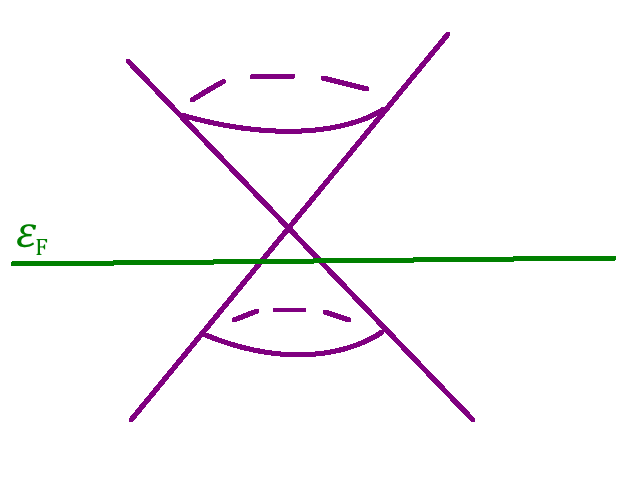
\includegraphics[width=2.5in]{Generic2.png}
 \end{center}
\caption{\small 一般地，3 维空间中拓扑绝缘体边缘局域模的能带交叉点并不出现在费米能处。
因此，边界与普通金属有许多共同之处。\figloc{19}{26}}
 \label{specialo}
\end{figure}

\subsection{离散晶格对称性与无质量狄拉克费米子}\label{dlat}

由于哈密顿量不必是洛伦兹不变的，我们实际上还没有找到在凝聚态物理中产生无质量狄拉克
费米子的办法，即便假定了时间反演对称性并调节一个参数。
然而，如果假定更多的对称性，无质量狄拉克费米子就可以变得自然。下面我们概述 \cite{YN}
中的一个构造，把一些细节留给读者。部分背景可参见 \cite{ASSS}。


首先，让我们重新考虑 $3+1$ 维中的相对论性无质量狄拉克费米子。哈密顿量为
$H=\g_0\vec \gamma\cdot \vec p$，其中现在 $\g^\mu$ 是 $4\times 4$ 矩阵，并假定不作手征
投影。等价地，该哈密顿量与下式共轭：
\be\label{perf}H=\bp \vec\sigma\cdot \vec p & 0 \cr 0 & -\vec\sigma\cdot\vec p\ep.\ee
其能级为 $\pm|\vec p|$，每个能级都以 2 重简并出现。

% [Tutor Note: 术语——克拉默斯（Kramers）简并的标准论证要点：$\sT$ 单独把 $\vec p$ 映到
% $-\vec p$，故在一般 $\vec p$ 处并不保证简并；只有使 $\vec p$ 固定的反幺正对称性
% （这里是 $\sP\sT$）才能在每个 $\vec p$ 处给出 Kramers 对。注意 $(\sP\sT)^2=-1$ 依赖
% 自旋 $1/2$（即 $\sT^2=-1$）；对整数自旋（或自旋 $1/2$ 的偶数个副本）有
% $(\sP\sT)^2=+1$，此时不产生 Kramers 简并。正文未加限定，读者宜按此理解。]
能带二重简并的一种解释如下。无质量非手征狄拉克哈密顿量同时具有时间反演对称性 $\sT$
与宇称对称性 $\sP$。这两者都使空间动量反号，因此乘积 $\sP\sT$ 在任一给定动量处都是
对称性。但 $\sP\sT$ 是反幺正对称性，并且在作用于费米子态时，$(\sP\sT)^2=-1$。
存在一个使 $\vec p$ 固定、平方为 $-1$ 的反幺正对称性，意味着每个动量处的能级具有
克拉默斯（Kramers）简并，这就解释了能带为何具有二重简并。

在凝聚态物理中，考虑一个具有 $\sPT$ 对称性的材料是完全自然的。的确，许多非磁性材料
具有 $\sT$ 对称性，许多晶体具有 $\sP$ 对称性（在凝聚态语境中通常称为反演对称性）。
在 $\sPT$ 对称的材料中，所有能带都将具有 2 重简并。如果可以忽略自旋-轨道力，这不过是
自旋导致的 2 重简并。然而，即使计入自旋相关的力，$\sPT$ 对称性也迫使所有能带具有严格的
2 重简并。


问题于是来了：在 $\sPT$ 对称的材料中（暂时假定没有其他对称性），能带这种一般的 2 重
简并会不会在布里渊区中某处变成 4 重简并？为回答这个问题，我们考虑一个具有 4 条能带的
一般 $\sPT$ 对称系统。作用于 4 个态（即在给定 $\vec p$ 值处 4 条能带的态）上的酉群一般
是 $U(4)$。这个群中与满足 $(\sPT)^2=-1$ 的反幺正对称性 $\sPT$ 对易的子群是 $Sp(4)$。
那十五个可能提升能带简并的 $4\times 4$ 无迹厄米矩阵在 $Sp(4)$ 下按
${\mathbf {15}}={\mathbf{5}}\oplus {\mathbf{10}}$ 变换。$\sPT$ 不变的那些按
${\mathbf{5}}$ 变换。事实上，群 $Sp(4)$ 是 $SO(5)$ 的双重覆盖 $\mathrm{Spin}(5)$，
而 $Sp(4)$ 的 ${\mathbf{5}}$ 正是 $SO(5)$ 的定义 5 维表示。

% [Tutor Note: 术语——文中 $Sp(4)$ 指紧致辛群（四元数酉群 $USp(4)$），其李代数为 10 维
% 紧致实形式 $\mathfrak{sp}(4)$，与实辛群 $Sp(4,\R)$（同为 10 维但非紧）不可混用；
% $\mathfrak{sp}(4)\cong\mathfrak{so}(5)$，故 $Sp(4)\cong\mathrm{Spin}(5)$ 是 $SO(5)$
% 的双重覆盖。原文只写 "the subgroup ... is $Sp(4)$"，未声明紧致性，读者易与实辛群混淆。]
% [Tutor Note: 含糊——${\mathbf{15}}={\mathbf{5}}\oplus{\mathbf{10}}$ 的分解作者未给推导。
% 其实质是：无迹厄米 $4\times4$ 矩阵构成 $\mathfrak{su}(4)$ 的 15 维伴随表示，在
% $Sp(4)\subset SU(4)$ 下分解成 ${\mathbf{10}}$（$Sp(4)$ 的伴随，与反幺正对称性 $\sPT$
% 反对易，正是会劈裂 Kramers 对的那部分）与 ${\mathbf{5}}$（与 $\sPT$ 对易，故保持 2 重
% 简并，但可使之整体升降）。下一段取的五块 $\h\g_i$ 就是这 ${\mathbf{5}}$ 的一组基。]
作为 5 个无迹、厄米、$\sPT$ 不变的 $4\times 4$ 矩阵的一组基，我们可以取伽马矩阵\footnote{我们在
这些伽马矩阵上加帽子，是因为它们与相对论描述中所用的 $SO(3,1)$ 伽马矩阵并不相同。
二者的关系在式 (\ref{preet}) 中说明。} $\h\g_1,\dots,\h\g_5$，
它们服从 $\{\h\g_i,\h\g_j\}=2\delta_{ij}$。因此一般的 $\sPT$ 不变、无迹的 4 带哈密顿量
为
\be\label{gert}H=\sum_{i=1}^5A_i(\vec p)\h\g_i.  \ee
要得到 4 重能带简并，我们需要使五个函数 $A_i(\vec p)$ 同时为零。一般地，在 3 维空间中，
这不会在布里渊区中任何地方发生。因此，要得到无质量狄拉克费米子，我们需要假定更多的
对称性。

让我们考虑一个具有 $\Z_n$ 旋转对称性的晶体，其中最方便的 $n$ 值\footnote{对 $n=3$ 也有
类似的情形，只需稍作修改。}是 4 与 6。我们假定所关心的能带简并出现在 $\Z_n$ 不变的
动量值处。（一般地，只有 $\Z_n$ 中保持给定能带简并所在动量不变的那个子群，才与保护
该简并有关。）我们可以安排晶轴，使 $\Z_n$ 保持 $p_1$ 不变。我们也可以不失本质地假定：
将出现无质量费米子的那个 $\Z_n$ 不变动量值满足 $p_2=p_3=0$。进一步，我们可以假定在
$p_2=p_3=0$ 附近，$\Z_n$ 由元素 $R$ 生成，$R$ 作用为 $p_2-p_3$ 平面的 $2\pi/n$ 旋转，
并保持 $p_1$ 不变。

$R$ 将在 4 条费米子能带上实现为 $Sp(4)$ 的一个元素；它将作用在 5 个伽马矩阵上，实现为
$SO(5)$ 的一个元素。$SO(5)$ 的一个 $n$ 阶一般元素，在 ${\mathbf 5}$ 表示中具有本征值
$1, $ $\exp(\pm 2\pi \i r/n)$, $\exp(\pm 2\pi \i s/n)$，其中 $r,s$ 是某些整数，我们可以
取它们非负且\footnote{我们可以进一步限制 $r\leq n/2$。
我们本可以把 $r,s$ 都限制为 $\leq n/2$，但那样就必须在下面的式 (\ref{mulch}) 中计入
一个可能的整体负号，因为作用于能带上的群 $Sp(4)$ 是作用于伽马矩阵上的群 $SO(5)$ 的
双重覆盖。} $\leq n$。由于我们马上要解释的理由，可以假定 $r+s$ 为奇数。
不同的情形对凝聚态物理都有意义，但要得到无质量狄拉克费米子，我们需要 $r$（或 $s$）等于
1，而另一个非零。既然 $r+s$ 为奇数，若 $r=1$ 且 $s\not=0$，则 $s$ 为偶数且 $\geq 2$。

$r+s$ 应为奇数的理由如下。若伽马矩阵在 $R$ 下按 $1,$ $\exp(\pm 2\pi \i r/n)$、
$\exp(\pm 2\pi\i s/n)$ 变换，则它们所作用的 4 条能带在 $R$ 下按
$\exp(\pi \i(\pm r\pm s)/n)$ 变换。但在费米子上，人们要求 $R^n=-1$，这对应于 $r+s$
为奇数。当 $r=1$ 时，$R$ 作用于 4 条能带的本征值为
\be\label{mulch}\exp(\pm\pi \i/n)\exp(\pm 2\pi\i s'/n),~~~s'=s/2,\ee
其中 $s'$ 是整数，因为 $s$ 为偶数。
 

我们可以选取 5 个伽马矩阵的一组基，使得 $\h\gamma_1$ 是 $R$ 不变的，$\h\g_2-\h\g_3$
平面被 $R$ 旋转角度 $2\pi/n$，而 $\h\g_4-\h\g_5$ 平面被 $R$ 旋转角度 $2\pi s/n$。
现在让我们分析哈密顿量，先沿轴 $p_2=p_3=0$，然后稍稍偏离该轴。

在 $p_2=p_3=0$ 处，动量是 $R$ 不变的。唯一 $R$ 不变的伽马矩阵是 $\h\g_1$，所以一般的
$R$ 不变哈密顿量为 $H=\h\g_1 A(p_1)$。$A(p_1)$ 在某个 $p_1$ 值处有单零点是很自然的，
而无质量狄拉克费米子就出现在那里。把哈密顿量按 $p_2$ 与 $p_3$ 的幂展开，由于假定了
$r=1$，$\h\g_2-\h\g_3$ 平面的旋转方式与 $p_2-p_3$ 平面相同，于是哈密顿量可以有一项
$B(p_1)(\h\g_2p_2+\h\g_3p_3)$。$\h\g_4,\h\g_5$ 的系数因为 $s\geq 2$ 而直到 $p_2,p_3$
的更高阶才出现。因此在 $p_2,p_3$ 的线性阶，哈密顿量为
\be\label{wonder}H=A(p_1)\h\g_1+B(p_1)(\h\g_2p_2+\h\g_3p_3).\ee
在 $A(p_1)$ 的任何单零点处都存在一个无质量狄拉克费米子，只要 $B(p_1)\not=0$。

假定 $r$（或 $s$）等于 1 其实相当自然，理由如下。它给出了 4 条能带在 $R$ 下变换的结果
(\ref{mulch})。但若所关心的 4 条能带是 2 条空间能带与 2 个自旋态的张量积，这正是人们
所期望的结果。作用在自旋 1/2 粒子的自旋态上的 $2\pi/n$ 旋转，其本征值为
$\exp(\pm \pi\i/n)$；而这样的旋转作用于 $\sPT$ 不变系统中的 2 条空间能带，本征值将是
$\exp(\pm 2\pi \i s'/n)$，其中 $s'$ 为某个整数。

% [Tutor Note: 笔误——原文此处把五维伽马矩阵平面写作 $\h\g^4-\h\g^5$（上标），
% 而式 (\ref{preet}) 与前文一直用下标 $\h\g_4,\h\g_5$（它们按
% $\{\h\g_i,\h\g_j\}=2\delta_{ij}$ 定义，指标本应取下标）。数值上二者相同，仅为记号
% 不一致；同一句紧接着又回到 $m,m'$ 的讨论，可见指的就是式 (\ref{preet}) 中的 $\h\g_4,\h\g_5$。
% 正文照录原文。]
从相对论的观点看，对我们所发现的结果可以这样解释：微观上作为空间旋转的 $R$，在低能
有效理论中表现为空间旋转与手征对称性的组合。这个手征对称性在上面的分析中表现为
$\h\g_4-\h\g_5$ 平面的旋转，它出现在 $s\not=0$ 之时。为更充分地说明这一点，请注意：
$\sPT$ 不变相对论狄拉克哈密顿量 (\ref{olof}) 中的五项与式 (\ref{gert}) 中的五项之间的
关系，来自
\be\label{preet}\g_0\g_i=\h\g_i~ ~(i=1,2,3), ~-\i\g^0=\h\g_4,~\i\g_1\g_2\g_3=\h\g_5.\ee
因此，$\h\g^4-\h\g^5$ 平面的旋转就是相对论哈密顿量 (\ref{olof}) 中参数 $m$ 与 $m'$ 的
旋转。在相对论物理中，旋转这些参数的对称性通常称为手征对称性，而这样的对称性迫使费米子
质量为零。

在上述分析中，我们只用了 $\sPT$，而没有分别使用 $\sP$ 与 $\sT$ 对称性。如果一种材料
只有 $\sPT$ 对称性而没有分开的 $\sP$ 与 $\sT$ 对称性，或者材料两者都有、但所关心的
能带简并出现在 $\sPT$ 不变、却不分别具有 $\sP$ 或 $\sT$ 不变性的动量值处，这样做都是
恰当的。在确实
具有分开的 $\sP$ 与 $\sT$ 对称性的材料中，还可以有一种有趣的构造 \cite{YZ}，它支配
出现在同时在这两种对称性下不变的动量值处的能带简并。结果表明，必须考虑非点式对称性
（non-symmorphic symmetries，即本质上混合旋转与部分晶格平移的对称性）。
关于这一主题的入门介绍（集中于 2 维空间中的类似问题），见 \cite{YK}。

作为同时假定 $\sP$ 与 $\sT$ 对称性之后果的一个简单例子，我们重新考虑 \ref{df} 节
讨论过的普通绝缘体与拓扑绝缘体之间的相变。事实上，在同时具有 $\sP$ 与 $\sT$ 对称性
时\footnote{我们假定能带并非在 $\sP$ 下全为偶或全为奇，以致作为 $Sp(4)$ 的元素有
$\sP\not=\pm 1$。否则低能物理会相当不同。}，这个相变发生在狄拉克费米子质量穿过 0 之时，
而不是通过脚注 \ref{complicated} 所描述的更复杂途径。关键在于：$\sPT$ 对称性使我们能用
五个函数来表示哈密顿量，如式 (\ref{gert}) 那样（而要写出这种对应，只需按式
(\ref{preet}) 把相对论哈密顿量 (\ref{olof}) 用式 (\ref{gert}) 的五个函数 $A_i$
表示出来）。当我们假定分开的
$\sT$ 与 $\sP$ 对称性时，五个函数 $A_i$ 中只有一个\footnote{要看穿这一点，一个简单的
办法是注意：$\sP$ 必须是 $Sp(4)$ 中满足 $\sP^2=1$、$\sP\not=\pm 1$ 的元素。任何这样的元素
（除 $\sP=\pm 1$ 外）对伽马矩阵的作用为 $\mathrm{diag}(-1,-1,-1,-1,1)$（在共轭意义下），
因而恰好保持 $A_i$ 的一个线性组合不变。按写式 (\ref{olof}) 时所用的标准相对论约定，
$\sP$ 的作用为 $\sP\psi(t,\vec x)=\i\g^0\psi(t,-\vec x)$，而 $\sP$ 不变的耦合是
$A_4=m$。}，即 $A_4=m$，是 $\sT$ 与 $\sP$ 共同不变的。其他 $A_i$ 都是奇的，并在
$\sT$ 与 $\sP$ 共同不变的点 $\vec p=0$ 处为零。于是在 $\vec p=0$ 处，只要把 $m$ 这一个
参数设为 0，就能实现 4 重能带简并。


\subsection{能带哈密顿量的简单例子}

最后，我们给出几个能带哈密顿量的简单例子，以说明上述一些想法。

一个目标是描述一个简单的能带哈密顿量，使它在 $\vec p=0$ 附近可以用手征狄拉克哈密顿量
$H=\vec\sigma\cdot \vec p$ 近似。为此，能带理论与相对论问题之间的主要差别在于：能带
理论中动量的各分量是周期变量。我们假定晶格间距为 $a$ 的简单立方晶格，于是动量的线性
分量的周期为 $2\pi/a$。要写下一个能带哈密顿量，我们可以把电子动量的线性分量 $p_i$，
$i=1,2,3$，替换为 $\frac{1}{a}\sin (p_ia)$，它具有正确的周期性，并在小 $p_i$ 时与 $p_i$
等价。这就启发我们写出能带哈密顿量
\be\label{twof}H=\frac{1}{a}\sum_{i=1}^3 \sigma_i\sin(p_ia).  \ee
公式 $\sin u=(e^{\i u}-e^{-\i u})/2\i$ 表明，写成坐标空间形式时，这个哈密顿量描述立方
晶格上的最近邻跃迁。

% [Tutor Note: 易错——正文断言式 (\ref{twof}) 的 8 个外尔点中"4 正 4 负"，可用 1.2 节的
% 手征性判据 (\ref{perd}) 核验：此处 $\vec b_i=\frac1a\sin(p_ia)$，故
% $\partial b_i/\partial p_j=\cos(p_ia)\delta_{ij}$，
% $\sign\det(\partial b_i/\partial p_j)=\sign\prod_{i=1}^3\cos(p_ia)$。于是
% $p_i\in\{0,\pi/a\}$ 中取 $\pi/a$ 的分量为偶数个者（共 $1+3=4$ 个）手征性为正；
% 为奇数个者（共 $3+1=4$ 个）手征性为负。
% 净手征性 $4-4=0$，与 Nielsen-Ninomiya 定理一致。]
对 $\vec p\to 0$，这个哈密顿量可用 $\vec\sigma\cdot \vec p$ 近似，所以在 $\vec p=0$ 处
有一个正手征性的外尔点。不过稍加思索即可看出，这个模型在布里渊区中实际上共有 8 个外尔
点；它们就是各个 $p_i$ 分别等于 0 或 $\pi/a$ 的那 8 个点。用判据 (\ref{perd})，读者可以
验证：这 8 个外尔点中 4 个具有正手征性，4 个具有负手征性。因此净手征性为 0，与
尼尔森-二宫定理相符。的确，尼尔森-二宫定理正是受诸如此类的例子的启发而提出的。

我们可以类似地写出非手征四分量狄拉克哈密顿量 (\ref{olof}) 的周期化版本：
\be\label{ollof}H=\frac{1}{a}\sum_{i=1}^3\g_0\gamma_i\sin(p_ia) -\i m\g^0. \ee
我们已取 $m'=0$，以保证 $\sT$ 与 $\sP$ 不变性（假定 $m$ 是 $\vec p$ 的偶函数）。若 $m=0$，
则在和先前相同的 8 个点处有无质量狄拉克费米子。若 $m$ 非零，则系统对所有 $\vec p$ 都有
能隙。它是绝缘体；而且若 $m$ 为常数，它事实上是平庸绝缘体。然而，若 $m$ 是 $\vec p$ 的
某个更一般的周期函数，我们就会得到新东西。假定 $m$ 很小，则 $H$ 中正比于 $m$ 的项只在
支撑着近无质量狄拉克费米子的那 8 个点附近才重要。而且，真正重要的只是 $m$ 在这 8 个点处
的符号。我们希望 $m(\vec p)$ 在 $\exp(\pm \i p_ia)$ 的幂下具有有限的傅里叶展开（从而
坐标空间哈密顿量是有限程的）。即使有这个限制，在 8 个所关心的点处独立地改变
$m(\vec p)$ 的符号也没有任何困难。当其中某个符号穿过 0 时，就会出现或消失一个边缘局域
的无质量狄拉克费米子。因此，这个带有适当函数 $m(\vec p)$ 的哈密顿量给出了 3 维空间中
拓扑绝缘体的一个简单模型。

% [Tutor Note: 术语——原文 ordinary insulator 与 trivial insulator 混用（如本节 "a trivial
% one" 与 1.11 节的 "ordinary insulator"），指的是同一类相：与拓扑绝缘体相对、可由绝热
% 连通到原子极限的绝缘体。译文分别照译为"普通绝缘体"与"平庸绝缘体"，以保留原文用词差异，
% 读者不必视其为两种不同的相。]
我们所描述的与霍尔丹（Haldane）关于 2 维空间中拓扑非平庸能带绝缘体的模型
\cite{Haldane} 有些类似。我们将在 \ref{hmg} 节回到那个模型。




% ======================================================================
%  第二讲 2.1-2.3：陈-西蒙斯有效作用量、耦合的量子化、霍尔电导率的量子化
% ======================================================================
\section{第二讲}

\begin{keytakeaways}
  \item 本讲从有效场论解释整数量子霍尔效应为何存在：若 2+1 维材料除电磁规范场外没有
        其他相关自由度，则其低能有效作用量中唯一“被积函数不规范不变、而积分仅在相差
        全导数意义下规范不变”的项，就是陈-西蒙斯项。
  \item 把理论放在二维球面与时间圆周的乘积上考察，可以显出大规范变换使陈-西蒙斯
        作用量平移一个完整周期的整数倍；由此其系数（级）必须为整数。
  \item 对电磁规范场变分即得诱导电流，霍尔电导率被量子化为 $k/(2\pi)$
        （以 $e^2/h$ 为单位即 $k$ 个基本电导量子），这是整数量子霍尔效应的宏观解释。
  \item 分数量子霍尔效应无法只用电磁场描述：需要引入仅在材料内部传播的演生规范场；
        朴素地把它积掉可得到分数霍尔电导率，但该推导有整体性缺陷，分数电荷与拓扑简并
        都要求保留该演生场。
  \item 同一整数在微观上就是 TKNN 不变量，即填充带复向量丛的第一陈类在布里渊区上的
        积分；2.4-2.5 节借助“宏观布里渊区”上的贝里联络给出另一种证明。
  \item 量子霍尔体系的边界上存在手征无能隙边缘模，右行与左行模数目之差等于陈-西蒙斯级 $k$；它们为
        抵消陈-西蒙斯项在边界上丢失的规范不变性所必需，是“反常流入”的例证。
\end{keytakeaways}

\subsection{陈-西蒙斯有效作用量}

今天我们从整数量子霍尔效应的若干方面讲起。首先，我只想从有效场论的观点说明：
整数量子霍尔效应究竟为何存在。我们考虑这样一种材料：它不仅绝缘，而且更进一步，
没有任何相关自由度——连拓扑自由度也没有；这里的意思是，它与电磁场的相互作用
可以只用电磁场的 $U(1)$ 规范场 $A$ 的有效作用量来描述，而不含任何额外自由度。
（对导体而言这当然不成立：要描述导体与电磁场的相互作用，除 $A$ 之外还必须把
载流子包括进来。但更微妙的是，正如我们将会讨论的，对分数量子霍尔体系也不成立：
其有效场论需要耦合到 $A$ 的拓扑自由度。）

在 $3+1$ 维、没有相关自由度的材料中，电磁场的有效作用量可以包含与各种熟知效应
相对应的各类项。例如，铁磁性与铁电性对应于有效作用量中关于 $\vec E$ 或 $\vec B$
线性的项
\be\label{dofof}I'=\int_{W_3\times \RR} \left(\vec a\cdot \vec E+\vec b\cdot \vec B\right).\ee
（这里 $W_3$ 是材料的空间体积，$\RR$ 参数化时间，因此材料的“世界体积”为
$M_4=W_3\times \RR$。）类似地，电极化率与磁化率对应于关于 $\vec E$ 或 $\vec B$ 的双线性项：
\be\label{moof}I''=\int_{W_3\times \RR}\left(\alpha_{ij} E_iE_j+\beta_{ij}B_iB_j\right).\ee
依此类推。

% [Tutor Note: 易错——原文未明说定向，本译注按 $\epsilon^{012}=+1$（即 $x_0,x_1,x_2$
%  为右手正序）阅读。若改用相反定向 $\epsilon^{012}=-1$，则 (2.3)、(2.15)、(2.16) 等含
%  $\epsilon^{ijk}$ 的项整体变号，霍尔电导率的符号随之反转；(2.4) 这类恒等式两边同时变号，
%  形式不变。核对 (2.15) 时务必与定向约定一并检查。]
所有这些项都明显地规范不变：它们是规范不变函数的积分，被积函数只由 $\vec E$ 与
$\vec B$（可能还有它们的导数）构成。在 $2+1$ 维中，存在唯一一个规范不变、却不具备
这一性质的项。
% [Tutor Note: 易错——陈-西蒙斯作用量的归一化固定为 $1/(4\pi)$：
%  $I_{\mathrm{CS}}=\frac{1}{4\pi}\int\epsilon^{ijk}A_i\partial_jA_k\,\d^3x
%  =\frac{1}{4\pi}\int A\wedge \d A$。若误用 $1/(2\pi)$ 的归一化，则 (2.14) 的 $k$
%  与 (2.15) 的霍尔电导率 $k/2\pi$ 都会差一个因子 2。]
这就是陈-西蒙斯耦合
\be\label{worf}\ICS=\frac{1}{4\pi}\int_{M_2\times \RR}\d^3x \epsilon^{ijk}A_i\partial_j A_k.\ee
被积分的密度 $ \epsilon^{ijk}A_i\partial_j A_k$ 绝不是规范不变的，但该积分在相差
一个全导数的意义下规范不变。
事实上，在
$A_i\to A_i+\partial_i\phi,$
之下，我们有
\be\label{omp} \epsilon^{ijk}A_i\partial_j A_k\to \epsilon^{ijk}A_i\partial_j A_k +\partial_i\left(\epsilon^{ijk}\phi\partial_jA_k\right).\ee

粗略地说，这表明 $\ICS$ 是规范不变的；但由于电荷量子化，我们必须更加小心。如果
电荷的量子由电荷为 1 的场 $\psi$ 携带，其变换为
\be\label{perrf}\psi\to e^{\i\phi}\psi,\ee
那么我们就应当认为 $\phi$ 只在模 $2\pi$ 的意义下有定义：
\be\label{eqr}\phi\cong\phi+2\pi.\ee
有鉴于此，前面那个假定 $\phi$ 为单值的、关于 $\ICS$ 规范不变性的证明并不完全正确。
稍后我们会更仔细地处理。

不过，在继续之前，我想指出：从逻辑上讲，人们可以考虑这样一种理论，其中只允许作
规范变换 $A_i\to A_i+\partial_i\phi$，而 $\phi$ 是单值的。但那样的理论不是真实世界。狄拉克（Dirac）
证明，电子、质子与中子的薛定谔（Schrödinger）方程可以自洽地与磁单极子耦合；
而这种自洽性之所以可能，正是因为薛定谔方程在 $e^{\i\phi}$ 单值、而 $\phi$ 本身不单值的
那些规范变换下不变。唯有如此，狄拉克弦才不可观测（图 \ref{DString}）。

  \begin{figure}
 \begin{center}
   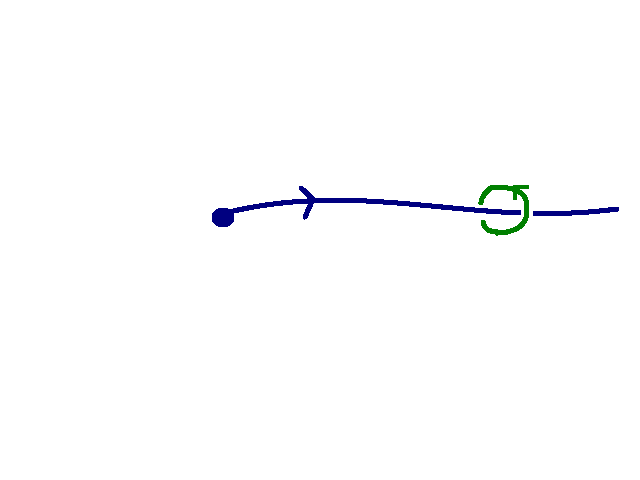
\includegraphics[width=2.5in]{DiracString.png}
 \end{center}
\caption{\small  从磁单极子发出的狄拉克弦不可观测，因为自然规律在 $e^{\i\phi}$ 单值、
而 $\phi$ 不单值的规范变换下不变。\figloc{20}{32}}
 \label{DString}
\end{figure}

无论如何，我们关于薛定谔方程在使 $e^{\i\phi}$ 单值的任何规范变换（即使 $\phi$ 不单值）
下不变的微观知识，会对有效作用量施加约束；若没有这一知识，我们就得不到这些约束。
我们想要理解这些约束。

\subsection{陈-西蒙斯耦合的量子化}

为此，我们考虑如下情形：把二维材料取为一个闭二维流形，例如 $S^2$；并把“时间”
取为周长为 $\beta$ 的圆周 $S^1$。（例如，我们可能正在计算 $\Tr\,e^{-\beta H}$。）于是我们
考虑其“世界体积”为 $M_3=S^2\times S^1$ 的材料（图 \ref{ST}）。

\begin{figure}
 \begin{center}
   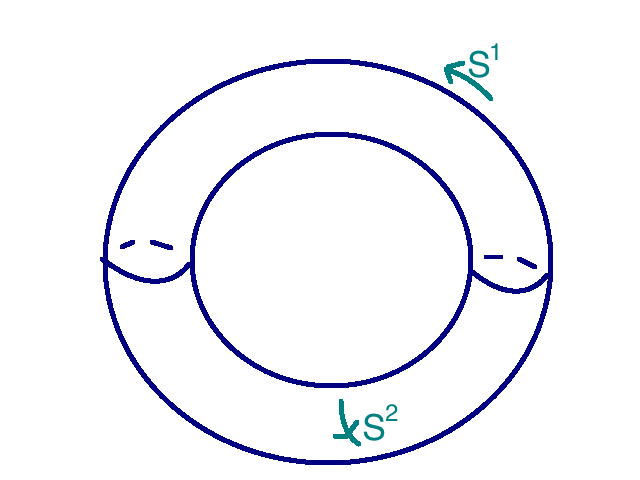
\includegraphics[width=2.5in]{Spacetime.png}
 \end{center}
\caption{\small 用于分析陈-西蒙斯作用量规范不变性的 $2+1$ 维流形 $S^2\times S^1$。\figloc{21}{32}}
 \label{ST}
\end{figure}

% [Tutor Note: 笔误——原文此处作 “Schdrodinger equation”，应为 “Schrödinger
%  equation”；同一段文字中另有 “magnetc”（应为 magnetic）、“quantitities”（应为
%  quantities）等拼写笔误，均不影响内容。]
人们也许无法在真实世界中构造出这种情形，但薛定谔方程在此情形下显然有意义。因此，
在推导由薛定谔方程可能给出的、对有效作用量的约束时，我们可以考虑这种情形。

我们想要在 $M_3=S^2\times S^1$ 上考虑的规范场如下。我们在 $S^2$ 上放置一个单位狄拉克磁通量：
\be\label{unitf}\int_{S^2}\d x_1 \d x_2\,\,\frac{F}{2\pi}=1.\ee
（若电子的协变导数为 $D_i\psi=(\partial_i-iA_i)\psi$，这就是正确的通量量子；这意味着我把通常记作 $eA$
的量写成了 $A$。这样就能在许多公式中避免 $e$ 因子。）

并且我们在 $S^1$ 或时间方向上取常数规范场：
\be\label{nif}A_0=\frac{s}{\beta},\ee
其中 $s$ 为常数。
% [Tutor Note: 笔误——脚注中的 $\partial A_i/\partial_s$ 与 (2.8) 的 $A_0=s/\beta$
%  不一致：按 (2.8) 应为 $\partial A_i/\partial s=\delta_{i0}/\beta$，其中 $\beta$ 来自
%  时间积分（$\int_0^\beta\d t$ 给出因子 $\beta$，故 $\partial\ICS/\partial s=1$ 的结论
%  不变）。若照字面取 $\delta_{i0}$，则会得到 $\partial\ICS/\partial s=\beta$ 而不是 1，
%  故原文疑漏写 $1/\beta$。又，若不理会狄拉克弦、直接用 $I_{\mathrm{CS}}
%  =\frac{1}{4\pi}\int A_0F_{12}$ 求值，会误得 $s/2$；脚注所说“棘手”正在于此，稳妥
%  做法是如脚注那样用 $F_{jk}$ 的变分。]
对这个规范场，可以算出\footnote{这实际上是一个稍嫌棘手的计算，因为 $S^2$ 上存在
非零磁通量时，规范场 $A_i$ 带有狄拉克弦奇点。一种稳妥的做法是计算 $\ICS$ 对
$s$ 的导数，利用对 $A$ 作任何无穷小变分时都有 $\delta \ICS=(1/4\pi)\int \epsilon_{ijk}\delta A_i F_{jk}$，而此式只用规范不变量
$F_{jk}$ 与 $\delta A_i$ 写出。将此公式用于 $\delta A_i=\partial A_i/\partial_s=\delta_{i0}$、且 $S^2$ 上有一个单位磁通量的情形，
可得 $\partial\ICS/\partial s=1$。再结合 $\ICS$ 在 $s=0$ 处为零这一事实，就得到式 (\ref{nifty})。}：
\be\label{nifty}\ICS= \frac{1}{4\pi}\int_{M_3=S^2\times S^1}\d^3x \epsilon^{ijk}A_i\partial_j A_k=s.\ee

注意 $A$ 绕“时间”圆周的和乐为
\be\label{wiff}\exp\left(i\int_0^\beta A_0\d t \right)=\exp\left(i\int_0^\beta (s/\beta)\d t\right)=\exp(is).\ee
规范变换
\be\label{rif}\phi= \frac{2\pi t}{\beta},\ee
（它被选来使 $e^{i\phi}$ 具有周期性）的作用为
\be\label{prif}s\to s+2\pi \ee
因而使和乐保持不变。（这一点必然成立，因为在我对 $A$ 的归一化下，该和乐正是
电子绕该圆周被平行移动一周时所获得的相位因子，因而具有物理意义。）

% [Tutor Note: 易错——(2.11) 的 $\phi=2\pi t/\beta$ 不是单值函数，但 $e^{i\phi}$ 单值，
%  故这是“大规范变换”：它把 $s$ 平移 $2\pi$（(2.12)），同时保持和乐 (2.10) 不变。
%  作用量 (2.9) 在此变换下恰平移 $2\pi$，这正是其系数 $k$ 必须为整数（(2.14)）的根源。
%  小规范变换（$\phi$ 单值）不产生这一限制。]
于是，在此例中 $\ICS=s$，而规范变换可以作用为 $s\to s+2\pi$。因此 $\ICS $ 并不完全规范不变；
它只是在模 $2\pi$ 的意义下规范不变。这里我们必须记住狄拉克在其磁单极子理论中所
利用的、本质上相同的事实。经典作用量 $I$ 只通过费曼路径积分中的因子 $\exp(\i I)$
（若恢复 $\hbar$，则为 $\exp(\i I/\hbar)$）进入量子力学，因此只要 $I$ 在模 $2\pi\Z$ 的意义下
良定义且规范不变就够了。由于 $\ICS$ 实际上正是在模 $2\pi \Z$ 的意义下规范不变（我们
在一个例子中证明了这一点，但它在一般情形下也成立），它可以在有效作用量中以整数
系数出现：
$$I_\eff=k\ICS+\dots.$$

\subsection{霍尔电导率的量子化}

% [Tutor Note: 术语——$k$ 在本文中称 “level”，译作“级”（陈-西蒙斯级）。它与能带论中
%  的“能级”(energy level) 无关；在量子霍尔语境中，$k$ 同时就是霍尔电导率的量子化整数
%  （以 $e^2/h$ 为单位，见 (2.15)）。]
这番解释的目的，是说明 $k$ 为何必须为整数——$k$ 有时被称为“级”。它取整数值
这一事实，给出了霍尔电流量子化的宏观解释。事实上，对任何与电磁势 $A$ 的相互作用
由有效作用量 $I_\eff$ 支配的材料，材料中的诱导电流为
\be\label{curr}J_i=-\frac{\delta I_\eff}{\delta A_i}. \ee
我们关心的是下述情形：
\be\label{zurr}I_\eff=k\ICS=\frac{k}{4\pi}\int_{M_3}\d^3x \epsilon^{ijk}A_i\partial_jA_k.\ee

\begin{figure}
 \begin{center}
   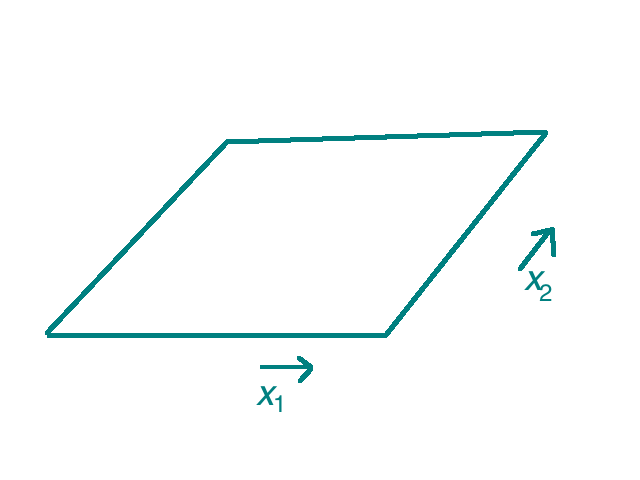
\includegraphics[width=2.5in]{Plane.png}
 \end{center}
\caption{\small 一个二维样品。\figloc{22}{34}}
 \label{SeT}
\end{figure}

% [Tutor Note: 易错——(2.15) 左端写作 $J_2=-\delta I_\eff/\delta A_1$，但按
%  $\epsilon^{012}=+1$ 直接变分 (2.14) 得 $\delta I_\eff/\delta A_1
%  =-\frac{k}{2\pi}F_{02}$、$\delta I_\eff/\delta A_2=+\frac{k}{2\pi}F_{01}$：右端的
%  $kF_{01}/2\pi$ 对应的是对 $A_2$ 的变分，而非对 $A_1$ 的变分，故下标 $A_1$ 疑应为 $A_2$。
%  但只改下标还不够：若保留 (2.13) 的负号，$J_2=-kF_{01}/2\pi$，与原文右端的 $+kF_{01}/2\pi$
%  仍差一符号；欲得正号须同时调整 (2.13) 的电流定义或 $E_i$ 的号差约定。建议以
%  $\rho=\sigma_{xy}B=\frac{k}{2\pi}B$（即 $\sigma_{xy}=k/2\pi$，单位 $e^2/h$）为物理基准定号。]
让我们考虑一块静止于 $x_3=0$、因而由 $x_1,x_2$ 参数化的材料（图 \ref{SeT}）。
$x_2$ 方向上的电流为
\be\label{murr}J_2=-\frac{\delta I_\eff}{\delta A_1}=\frac{kF_{01}}{2\pi}=\frac{kE_1}{2\pi}. \ee
这被称为霍尔电流：$x_1$ 方向的电场产生了 $x_2$ 方向的电流。霍尔电流具有量子化的
系数 $k/2\pi$（通常记作 $ke^2/h$；回忆一下，我的 $A$ 通常记作 $eA$，而我取
$\hbar=1$，故 $h=2\pi$），其量子化来自 $\ICS $ 并不完全规范不变这一事实。

% [Tutor Note: 笔误——原文此段作 “One cannot get an integer quantum Hall effect in a
%  description in which $A$ is the only relevant degree of freedom.”，但上下文（问“如何
%  能有分数量子霍尔效应”，随后即引入演生规范场 $a$）表明此处 “integer” 疑应为
%  “fractional”。译文照原文直译，未作改动。]
人们或许会问：“那么，怎么能有分数量子霍尔效应呢？”目前我先给出一个简短的回答，
把更多细节留到第三讲。\footnote{关于分数量子霍尔效应有效场论这一极为丰富的主题
（附有截至当时的文献指引），可参见 \cite{Wen} 这篇有用的导论。} 在 $A$ 是唯一
相关自由度的描述中，无法得到整数量子霍尔效应。然而，从宏观上看，这可以发生在一种
材料中：该材料产生一个额外的、“演生的” $U(1)$ 规范场 $a$，它只在材料内部传播。
我们归一化 $a$，使它具有与 $A$ 相同的通量量子，即\footnote{
% [Tutor Note: 术语——把演生规范场 $a$ 的规范群取为紧致的 $U(1)$（而非非紧致的
%  $\RR$）是分数量子霍尔有效场论的关键：紧致性允许“单极子算符”破坏
%  $\mathbf q=\int\d^2x\,f_{12}$ 的守恒，并使 $a$ 具有 $2\pi$ 的狄拉克通量量子，
%  从而 (2.16) 的 $r$ 必须为整数；若取非紧致 $\RR$，$\mathbf q$ 严格守恒，与凝聚态
%  物理不符。详见原脚注与 \cite{Wen}。]
在凝聚态物理的语境中，假定演生规范场 $a$ 所规范的是非紧致规范群 $\RR$ 而非
紧致规范群 $U(1)$，是不符合物理的。在那种情形下，会存在一个严格守恒的流 ${\mathbf j}_i=\frac{1}{2}\epsilon_{ijk}f^{jk}$；
相应地，空间积分
${\mathbf q}=\int\d^2x \,{\mathbf{j}}^0=\int\d^2x\, f_{12}$ 将是一个严格守恒的量。而在凝聚态物理中，并不存在可作为
$\mathbf q$ 候选者的严格守恒量。若演生规范群是 $U(1)$ 而不是 $\RR$，则可以把
“单极子算符”加入哈密顿量，从而破坏 $\mathbf q$ 的守恒。由于演生规范群是 $U(1)$，
存在非平庸的狄拉克通量量子；我们归一化 $a$，使该通量量子为 $2\pi$。据此，
式 (\ref{urr}) 中的参数 $r$ 必须为整数。}
$2\pi$。我们将用 $f_{ij}=\partial_ia_j-\partial_ja_i$ 表示 $a$ 的场强。
% [Tutor Note: 易错——(2.16) 中 $A\d a$ 混合项的系数是 $1/(2\pi)$，而纯 $a\d a$ 项
%  的系数是 $r/(4\pi)$，二者不对称并非笔误：前者对应 $\frac{1}{2\pi}\int A\wedge\d a$，
%  后者对应 $\frac{r}{4\pi}\int a\wedge\d a$。由 (2.16) 变分得到的运动方程是 (2.17)
%  的 $f=F/r$（注意是 $1/r$ 而非 $r$），这正是消去 $a$ 后霍尔电导率为 $1/r$ 的来源。]
一个导致分数量子霍尔效应的规范不变有效作用量的例子是
\be\label{urr}I_\eff=\frac{1}{2\pi}\int_{M_3}\d^3x\,\,\epsilon^{ijk}A_i\partial_j a_k -\frac{r}{4\pi}\int_{M_3}\d^3x\,\,\epsilon^{ijk}a_i\partial_j a_k . \ee

一个过分简化的、说明它为何给出分数量子霍尔效应的论证如下。人们论证道：由于 $a$
在有效作用量中只以二次形式出现，可以用它的运动方程把它积掉。该运动方程为
\be\label{yre}f=\frac{1}{r}F,\ee
这意味着在相差一个规范变换的意义下 $a=A/r$。把它代入 $I_\eff$，就得到只含 $A$
的、描述分数量子霍尔效应的有效作用量：
\be\label{zyre}I'_\eff=\frac{1}{r} \ICS(A)=\frac{1}{r}\frac{1}{4\pi}\int_{M_3}\d^3x \,\,\epsilon^{ijk}A_i\partial_jA_k.\ee

% [Tutor Note: 含糊——作者说 $f=F/r$ 一般不能整体解出 $a$，因为 $F$ 与 $f$ 的允许
%  通量量子同为 $2\pi$；其数学实质是 $A$ 与 $a$ 都是非平庸 $U(1)$ 丛上的联络，
%  $\int F/2\pi$ 与 $\int f/2\pi$ 的整数值可以不匹配，“积掉 $a$”只在局部（或忽略
%  拓扑扇区时）成立。因此 $a$ 不能被真正消去；分数电荷与拓扑简并都必须保留 $a$。
%  详见第三讲与 \cite{Wen}。]
这里，在通常出现 $k$ 的位置出现了 $1/r$，这暗示该模型中的霍尔电导率为 $1/r$。
这是正确的。但这个推导显然有毛病，因为所声称的有效作用量 $I'_\eff=(1/r)\ICS(A)$ 并不合理：它破坏了
规范不变性。错误在于：一般情形下，由于 $F$ 可以带有 $2\pi$ 的通量量子，而
$f$ 具有与之相同的允许通量量子（否则我们假定的作用量就不会规范不变），对给定
的 $A$，无法从方程 (\ref{yre}) 解出 $a$。于是，不可能从该系统中消去 $a$、
只用 $A$ 来给出描述。“积掉 $a$”之所以能给出霍尔电流的正确结果，是因为这一
做法在局部成立，而这就足以确定霍尔电流。该系统还具有更微妙的性质（带分数电荷的
准粒子与拓扑简并），只有在同时包含 $a$ 与 $A$ 的描述中才能正确理解。第三讲
将介绍这些性质。

% ======================================================================
%  第二讲 2.4-2.6：与能带拓扑的关系、等价性的证明、边缘态与反常流入
% ======================================================================
\subsection{与能带拓扑的关系}

回到可以只用 $A$ 描述的理论，我们在宏观描述中有一个整数 $k$。但在能带绝缘体的
微观描述中还有另一个整数，即 TKNN 不变量 \cite{TKNN}。它来源于如下考虑。我们考虑一个
有 $N$ 个能带、其中 $n$ 个被填充的晶体。我们假定系统对所有动量值都完全有能隙。
正如昨天所学，在二维系统中，没有能带交叉是一般情形。

% [Tutor Note: 术语——TKNN 不变量 \cite{TKNN} 在此定义为第一陈类 $c_1(\H'_p)$ 在布里渊区
%  上的积分，即填充带复向量丛的陈数 $k'=\int_\B\Tr\F/2\pi$。文献中 $c_1$ 有时指上同调类、
%  有时指其积分（陈数），本文取后者，$k'$ 为整数。注意别与第一讲的缠绕数（$\pi_2(S^2)$
%  的映射度）混淆：在二能带模型中二者数值一致。]
我们与昨天讨论外尔半金属时所处的情形相同，只是这里没有能带交叉点，因此我们在整个
布里渊区 $\B$ 上工作，不必挖去任何点。由于是二维，$\B$ 是一个二维环面。在动量
$p$ 处，令 $\H_p\cong \C^N$ 为所有态构成的完整空间，$\H'_p$ 为填充能级构成的子空间。我们可以
把 $\H_p$ 视为 $\B$ 上一个秩（或维数）为 $N$ 的“平凡丛”，而把 $\H'_p$ 视为一个
秩为 $n$ 的“子丛”。我们想要的整数——记作 $k'$——是 $c_1(\H'_p)$ 在 $\B$ 上的积分。
用我们昨天讨论过的、填充能带上的贝里联络 $\A$（其曲率我们记作 $\F$）来表达，这个
整数是
$$k'=c_1(\H'_p)=\int_\B \frac{\Tr\,\F}{2\pi}. $$

TKNN 的基本论断是：贝里联络的通量 $k'$ 与量子霍尔电流的系数 $k$ 相同。最初的
证明实质上就是按第一性原理、用费米子基态中的矩阵元来计算电流——该矩阵元写成单粒子
矩阵元在布里渊区上的积分。我想解释一个不同的观点，它将强调 $k'$ 不只是能带概念，
而可以在完整的多体理论中定义。（在第三讲中，我将描述另一种本质属于霍尔丹（Haldane）
的、处理 $k=k'$ 关系的方法。）

我们考虑一个有限样品，比如说放在 $n_1\times n_2$ 的格点上（图 \ref{Rectangular2}），其中
$n_1,n_2$ 非常大；两个方向的晶格常数取为 $a_1, a_2$。于是格点的物理尺寸为 $L_1\times L_2$，其中
$L_1=n_1a_1,$ $L_2=n_2a_2$。我们假定周期边界条件，以保持晶格平移对称性。然而对有限系统，动量
取离散值
\begin{align}\label{zudo}\notag p_1&=\frac{2\pi s_1}{L_1}, ~~0\leq s_1\leq n_1-1\cr
p_2 &=\frac{2\pi s_2}{L_2}, ~~0\leq s_2\leq n_2-1.\end{align}
有限系统的基态当然就是填满前 $n$ 个能带中具有这些动量值的所有态所得到的态。

  \begin{figure}
 \begin{center}
   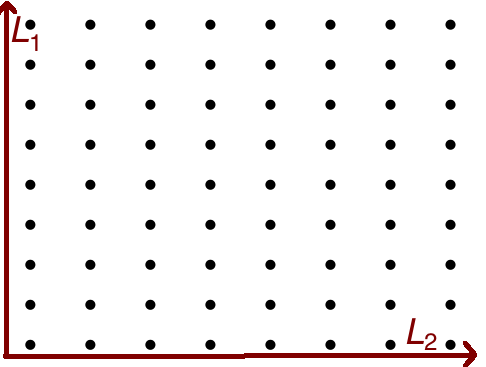
\includegraphics[width=2.5in]{Rectangular2.png}
 \end{center}
\caption{\small 大小为 $n_1\times n_2$ 的周期性格点，两个方向的晶格常数分别为 $a_1,a_2$。格点的
物理尺寸为 $L_1\times L_2$，其中 $L_1=n_1a_1, \,L_2=n_2a_2$。\figloc{23}{36}}
 \label{Rectangular2}
 \end{figure}

% [Tutor Note: 易错——$\alpha_1,\alpha_2$ 只在模 $2\pi$ 下定义：$\alpha_i\to\alpha_i+2\pi$
%  等价于 $s_i\to s_i+1$ 的整数平移，故其参数空间是环面 $\widehat\B$（“宏观布里渊区”），
%  而不是平面。这一等价性正是 2.5 节证明 $k'=\widehat k'$ 的关键：$\B$ 与 $\widehat\B$
%  只是同一组离散态的两种组织方式。]
但现在我们引入一个背景电磁矢势，其选择使得磁场为零，而电子沿 $x_1$ 方向或 $x_2$
方向绕行一整圈时都会获得一个相位：
$$A_1=\frac{\alpha_1}{L_1}, ~~  A_2=\frac{\alpha_2}{L_2}. $$
电子沿 $x_1$（或 $x_2$）方向绕行一周所获得的相位为 $\exp(i\alpha_1)$（或 $\exp(i\alpha_2)$）；在相差
一个规范变换的意义下，这些参数的取值范围是
$$0\leq \alpha_1 ,\,\,\alpha_2\leq 2\pi.$$

从能带理论的观点看，引入参数 $\alpha_1,$ $\alpha_2$ 的效应只是平移电子的动量，使其变为
$$p_1=\frac{2\pi s_1+\alpha_1}{L_1}, ~~0\leq s_1\leq n_1-1$$
$$p_2=\frac{2\pi s_2+\alpha_2}{L_2}, ~~0\leq s_2\leq n_2-1.$$
这实际上表明，谱在 $\alpha_1$ 或 $\alpha_2$ 平移 $2\pi$ 之下不变（只差 $s_1$ 或 $s_2$
的一个整数平移）。对任意 $\alpha_1,\alpha_2$，从能带理论的观点看，基态就是把前 $n$ 个能带中
具有这些平移后动量值的所有态都填满而得到的态。

现在我们把参数 $\alpha_1$、$\alpha_2$ 视为将要绝热变化的参数。由于它们各自只在模 $2\pi$
下定义，它们参数化一个环面，我把它记作 $\widehat \B$。（$\widehat \B$ 可以看作布里渊区 $\B$
的某种重新标度版本。）由于贝里（Berry）的构造对参数的绝热变化是普适的，我们可以在
$\widehat \B$ 上构造一个贝里联络 $\widehat {\A}$，其曲率为 $\widehat{ \F}$。$\widehat {\A}$ 是当参数
$\alpha_1,\alpha_2$ 变化时用来输运基态的联络。要定义它，我们只需知道基态在 $\alpha_1,\alpha_2$ 变化时始终非简并。我们
不需要假定单粒子图像（即能带理论）。但我应当说明：为使所得结论有用，至少以我将
陈述的形式而言，我们需要基态的能隙在 $L_1,L_2$ 变大时与它们无关。（否则，我们在实验室
中的测量实际上可能并不绝热。如第三讲将要讨论的，所述假定对分数量子霍尔体系并不
成立。）

% [Tutor Note: 易错——$\widehat\B$（macroscopic Brillouin zone）是 $\alpha_1,\alpha_2$
%  的参数环面；它与 $\B$ 上的贝里联络 $\A$（单粒子能带）不同：$\widehat{\A}$ 是基态随
%  $\alpha$ 绝热变化的联络，$\widehat{\F}$ 是其曲率。$\widehat k'$ 的定义不依赖能带图像
%  （可用于多体理论），这是作者强调其“更一般”的原因。另需注意：原文用 \A 与 \AA 两个
%  不同宏，但导言区把它们都定义为 \mathcal A，排版后同为 $\mathcal A$；阅读源码时须按
%  上下文区分“能带贝里联络”“参数空间联络”与“电磁矢势”。]
利用 $\widehat B$ 上的贝里联络，我们可以定义一个整数：
$$\widehat k' =\int_{\widehat B}\d\alpha_1\,\d\alpha_2\,\,\frac{\widehat \F}{2\pi}. $$

但我断言，它与能带理论中定义的整数 $k'$ 相同：
$$k'=\widehat k'.$$

这之所以有用，是因为 $\widehat k'$ 的定义更为一般。为定义 $k'$，我们假定了能带理论——
即基于自由电子的单粒子描述。而 $\widehat k'$ 的定义所需假定要少得多。

  \begin{figure}
 \begin{center}
   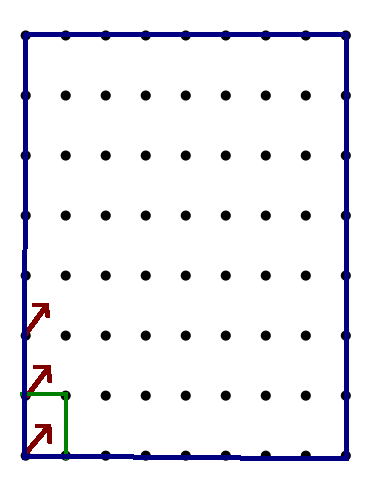
\includegraphics[width=2in]{RotatedLattice3.png}
 \end{center}
\caption{\small 大矩形（其对边应认同）表示参数化电子动量的动量空间布里渊区 $\B$。
左下角的小矩形（同样对边认同）表示参数化平移角 $\alpha_1$、$\alpha_2$ 的宏观布里渊区
$\widehat\B$。黑点是大小为 $n_1\times n_2$ 的有限格点所允许的动量取值（此处按 $n_1=8$、$n_2=7$
画出）。引入 $\alpha_1$ 与 $\alpha_2$ 会按箭头所示平移这些允许动量。特别地，图中左下角的
那一点可以被移动到代表 $\widehat \B$ 的小矩形内的任意位置。\figloc{24}{38}}
 \label{ShiftedLattice}
\end{figure}

\subsection{等价性的证明}

为理解 $k'=\widehat k'$ 的原因，我在图 \ref{ShiftedLattice} 中画出了布里渊区内满足有限体积
条件的离散点。参数 $\alpha_1,\alpha_2$ 参数化图中的一个小矩形，比如说左下角那个。

为计算 $k'$，我们在整个布里渊区 $\B$ 上积分。为计算 $\hat k'$，我们在小矩形上
积分，但对小矩形中的每一点，还要对相应的平移后动量求和。这是组织同一计算的两种
不同方式，因此 $\hat k'= k'.$
所以，与其证明原始的 TKNN 公式 $k=k'$，等价地只需证明
$k=\hat k'$。这有下述好处：$\hat k'$ 是用系统对变化的电磁矢势 $A$ 的响应来定义的，因此
我们只凭 $A$ 的有效作用量就能确定 $\hat k'$。

% [Tutor Note: 含糊——作者说作用量 (2.19) 中“更高阶的项不重要”，实质是绝热极限
%  $T\to\infty$ 下含两个或更多时间导数的项 $\sim 1/T^{m-1}\to 0$（可参下文对动能项
%  (2.20) 的估计 $\sim 1/T$）。取 $V(x)=0$ 是把讨论限制在零能态的经典构型子空间上，
%  这就是这里的半经典近似。]
作为练习，在确定 $A$ 的贝里联络之前，我先来确定一个具有动力学变量 $x^i(t)$ 的
任意动力学系统的贝里联络。可以把 $x^i(t)$、$i=1,\dots,3$ 设想为代表一个质点的位置坐标，
但它们实际上可以是任何东西（例如 $x^i(t)$ 可以有 $3N$ 个分量，代表 $N$ 个
质点的位置）。无论如何，我们假定作用量
\be\label{merrof}I=\frac{1}{2}\int\d t\, g_{ij}(x)\frac{\d x^i}{\d t}\frac{\d x^j}{\d t}+ \int \d t \AA_i(x) \frac{\d x^i}{\d t}-\int\d t V(x)+\dots.\ee
（可能还有更高阶的项，但稍后就会清楚它们并不重要。）我们将在零能的半经典态空间里
计算贝里联络；这一条件通过施加 $V(x)=0$ 来满足。（这一半经典近似在我们的问题中成立，
因为我们不需要把电磁矢势 $A$ 作量子处理。我们可以把它看作给定的外场。）

令 $V=0$ 意味着我们不是对所有的 $x$ 值、而只对保证 $V(x)=0$ 的 $x$ 值计算
贝里相位。因此我们从作用量中扔掉 $V(x)$ 项，只在位形空间中 $V=0$ 的子空间内进行
输运。在绝热输运中，我们还可以忽略作用量中的项
\be\label{monkey}I_{\mathrm{kin}} =\frac{1}{2}\int\d t\, g_{ij}(x)\frac{\d x^i}{\d t}\frac{\d x^j}{\d t}\ee
以及任何其他含两个或更多时间导数的项。这是因为，若在时间 $T$ 内从起点 $p$
输运到终点 $p'$，则导数 $\d x^i/\d t$ 为 $1/T$ 量级，因而 $I_{\mathrm{kin}}\sim 1/T$。在绝热极限
$T\to \infty$ 下它趋于零。

  \begin{figure}
 \begin{center}
   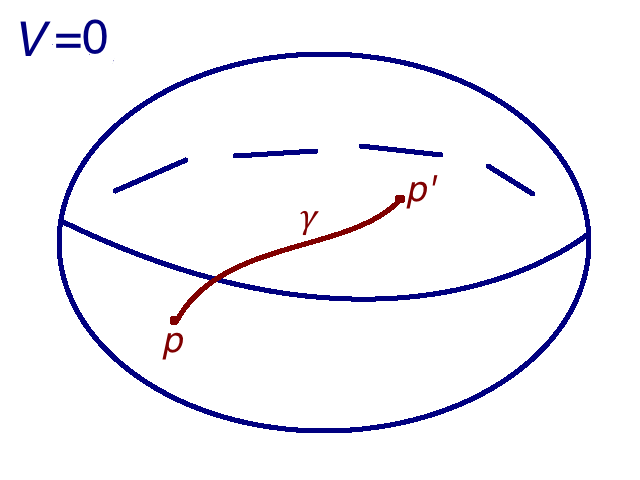
\includegraphics[width=2.5in]{Sub2.png}
 \end{center}
\caption{\small 量子粒子在位形空间中两点 $p$ 与 $p'$ 之间的传播。我们假定传播
发生在 $V=0$ 的子空间内，图中以二维球面表示该子空间。传播的粒子获得相位 $\exp(\i I/\hbar)$，
其中 $I$ 是所选轨道的经典作用量。\figloc{25}{39}}
 \label{traj}
\end{figure}

于是作用量中唯一需要保留的项，是恰好含一个时间导数的项：
\be\label{wonkey}I'=\int\d t \,\AA_i(x)\frac{\d x^i}{\d t}=\int_p^{p'}\AA_i(x)\d x^i.\ee
正如我所指出的，这一项只依赖于从 $p$ 到 $p'$ 所走的路径，而不依赖于路径如何
参数化。现在回忆一下：量子粒子沿给定轨道从 $p$ 传播到 $p'$ 所获得的相位是
$e^{\i I/\hbar}$，其中 $I$ 是该轨道的作用量（图 \ref{traj}）。对我们而言，在 $\hbar=1$ 的
单位制下，这个相位就是 $\exp\left(\i\int_\gamma\AA_i \d x^i\right)$。

但是，沿路径 $\gamma$ 平行移动时给出相位
$\exp\left(\i\int_\gamma\AA_i \d x^i\right)$ 的联络正是 $\AA$。换言之，我们了解
到：对于一个量子基态可以看作等价于经典基态的系统，贝里联络就是从经典作用量中读出的
经典联络 $\AA$。

% [Tutor Note: 易错——(2.22) 的麦克斯韦项写作 $\frac{1}{2e^2}\int(\vec E^2-\vec B^2)$，
%  这里的 $e$ 与 2.1 节的约定 $A\equiv eA_{\mathrm{phys}}$ 配套：因 $F=eF_{\mathrm{phys}}$，
%  麦克斯韦作用量正比于 $F^2/e^2$。若把 $A$ 直接理解为物理矢势，则该系数应改为 $1/2$
%  （或按所选单位调整）；此外 $e$ 在 $k\ICS$ 项中不出现，正因为该项已用 $A=eA_{\mathrm{phys}}$
%  写出。]
对本题中的电磁场，作用量为
\be\label{elfi}I=\frac{1}{2e^2}\int_{\RR^{3,1}}\d^3x \d t \left(\vec E^2 - \vec B^2\right) +\frac{k}{4\pi}\int_{W_3}\d^2x\d t \,\epsilon^{ijk}A_i\partial_j A_k+\dots  .\ee
我们假定，例如在两个方向上具有周期边界条件，其周期 $L_1,L_2$ 很长；这两个方向由我们的
量子霍尔样品填充。（第三个方向上是否假定周期边界条件无关紧要。）零能的经典态由前面
引入的两个角 $\alpha_1$、$\alpha_2$ 标记。为计算贝里相位，我们应当把此式代入作用量，
只保留恰好含一个时间导数的那部分作用量。这部分只来自陈-西蒙斯项。

% [Tutor Note: 易错——(2.23) 的系数 $-\frac{k}{2\pi}$ 与符号来自 (2.22) 的 CS 项在
%  $A_1=\alpha_1/L_1$、$A_2=\alpha_2/L_2$（随时间变化）下的取值：含一个时间导数的项为
%  $\frac{k}{4\pi}(-\alpha_1\dot\alpha_2+\alpha_2\dot\alpha_1)$，把 $\alpha_2\dot\alpha_1$
%  分部积分并丢掉全导数后得 $-\frac{k}{2\pi}\alpha_1\dot\alpha_2$。这个负号决定了
%  (2.25) 中 $\widehat\F=+k/2\pi$。]
对 $x_1$ 与 $x_2$ 积分后，作用量的相关部分就是
\be\label{mizz}I'=-\frac{k}{2\pi}\int\d t \,\alpha_1 \frac{\d \alpha_2}{\d t}.\ee
由此读出贝里联络
\be\label{roff} \nabla\equiv\left(\frac{D}{D\alpha_1},\frac{D}{D\alpha_2}\right)=\left(\frac{\partial}{\partial \alpha_1}, \frac{\partial}{\partial\alpha_2}+i\frac{k\alpha_1}{2\pi}\right),\ee
从而得到贝里曲率
\be\label{coff}\hat\F_{\alpha_1\alpha_2}=-i\left[\frac{D}{D\alpha_1},\frac{D}{D\alpha_2}\right]=\frac{k}{2\pi}.  \ee
（若给 $I' $ 加上一个全导数项 $\int \d t\, \partial_t f(\alpha_1,\alpha_2)$，这会改变 $\nabla$ 的公式，但不会改变
$\hat\F$。）

% [Tutor Note: 易错——(2.26) 的被积函数为 $\widehat\F/2\pi=\frac{k}{(2\pi)^2}$（常数），
%  积分区域 $\alpha_1,\alpha_2\in[0,2\pi]$ 的面积为 $(2\pi)^2$，故积分等于 $k$。这里的
%  $k$ 正是 (2.14) 中霍尔电导率的级，$k'=\widehat k'$ 由此得到验证。]
我们记得，整数 $\hat k'$ 应当是 $\hat\F/2\pi$ 在布里渊区上的积分。现在可以算出
\be\label{plizz}\hat k'=\int_0^{2\pi}\d\alpha_1\d\alpha_2\, \frac{\hat\F}{2\pi}= \int_0^{2\pi}\d\alpha_1\d\alpha_2\, \frac{k}{(2\pi)^2}=k.  \ee
于是我们得到了著名 TKNN 公式的一个版本：量子霍尔电流的系数 $k$ 可以表为贝里联络
的通量积分。

\subsection{边缘态与反常流入}

昨天我们解释了为什么纯粹一维的量子电子气不可能存在左行与右行电子激发之间的不平衡。
作为提醒：原因在于周期轨道上“有升必有降”（图 \ref{Crossings}）。从场论的观点看，
这是必需的，因为只有右行、没有左行的无能隙费米子无法以规范不变的方式量子化。存在
1+1 维版本的阿德勒-贝尔-杰基夫（Adler-Bell-Jackiw）反常 \cite{Adler,BJ}。

% [Tutor Note: 术语——“反常流入”（anomaly inflow）指体区一个在边界存在时并不规范
%  不变的作用量（此处为 $k\ICS$）与边界上一个反常理论（手征边缘模）互相补偿：边界反常
%  使体区的规范不变性缺陷无法被局部边界项消除。1+1 维的手征反常即 Adler-Bell-Jackiw
%  反常 \cite{Adler,BJ}；反常流入的文献见 \cite{CH}。]
然而，量子霍尔体系的标志之一，恰恰是它的边界上存在这种不平衡。这必然发生的原因是：
当我们验证陈-西蒙斯作用量
\be\label{facs}k\ICS=\frac{k}{4\pi}\int_{M_2\times \RR}\d^3x \epsilon^{ijk}A_i\partial_j A_k\ee
在规范变换 $A_i\to A_i+\partial_i\phi$ 下的不变性时，必须分部积分。这一分部积分会在材料表面上——即在
$\partial M_2\times \RR$ 上——产生一个表面项。我们无法通过给作用量加上一个支撑在
$\partial M_2\times \RR$ 上的表面项
来抵消这一规范不变性的破坏。你可以试着把 $\ICS$ 换成
% [Tutor Note: 含糊——(2.28) 中的 $?????$ 是作者有意留下的占位符，表示“$A$ 及其导数的
%  任意局部多项式”，并非排版错误；作者建议读者自行验证任何局部边界项都无法抵消
%  $\partial M_2\times\RR$ 上的规范不变性破坏。]
\be\label{trytry}\ICS+\int_{\partial M_2\times \RR}\d t\,\d x\left(?????\right),\ee
其中 $?????$ 是 $A$ 及其导数的某个多项式，但无论怎么试都不会成功。（我推荐做这个
练习。）正是因为这一反常无法通过加上边界上的某种局部相互作用来消除，该反常才具有
物理意义。

要抵消这一反常，即抵消 $\ICS$ 沿边界丢失的规范不变性，就要求边界上存在这样的模：
(1) 它们无能隙，因而不能被积掉以产生只含 $A$ 的局部有效作用量；(2) 它们是“反常的”，
即在纯粹一维系统中不可能存在。符合要求的，恰恰就是我们发现纯粹一维系统中并不存在的
东西：“手征费米子”，即没有左行模伴随的右行无能隙模。边界理论中的反常可以由体区中一个
在存在边界时并不规范不变的相互作用来抵消，这一事实是“反常流入”现象的例证 \cite{CH}。

% [Tutor Note: 易错——$n_+-n_-=k$ 中的 $n_\pm$ 分别按“右行/左行”无能隙边缘模计数；边缘模的
%  手征性必须与体区霍尔电导率的符号配对：若霍尔电导率取相反符号，则相应关系变为
%  $n_+-n_-=-k$。又，作者此处说“霍尔电导率为 $k$”，按 (2.15) 的约定应理解为 $k/2\pi$
%  （即 $ke^2/h$），是以 $k$ 为整数的简写。]
由于 $k\ICS$ 的规范不变性破坏正比于 $k$，用来抵消它所需的“手征不对称”也正比于
$k$。事实上，霍尔电导率为 $k$ 的整数量子霍尔体系的标志，恰恰是
$$n_+-n_-=k$$
其中 $n_+$ 与 $n_-$ 分别是“右行”与“左行”无能隙边缘模的数目。我打算给出几个可能
更物理的说明——今天一个，第三讲一个——而不是对场论反常作技术性分析来解释其机制。

\subsection{电荷泵}\label{tcp}

% [Tutor Note: 术语——“Thouless charge pump” 译作“索利斯电荷泵”。这里的 charge pump 指参数 $\alpha$ 绝热绕行一周时穿过某一截面的净电荷；Thouless \cite{Thouless} 证明该电荷为整数，这是 TKNN 不变量的输运表述，与 2.6 节（边缘态与反常流入）的论证互为表里。不要把它与器件意义上的“量子泵”、或 $\alpha$ 本身的周期性混为一谈。]
今天的解释涉及索利斯（Thouless）电荷泵 \cite{Thouless} 的一个版本。
让我们考虑一个位于长圆柱面上的量子霍尔系统。事实上，作为开始，先考虑一个无限长圆柱（图
\ref{Cylinder}）。

   \begin{figure}
 \begin{center}
   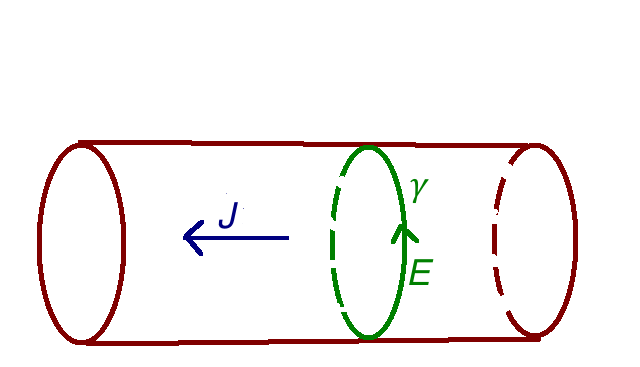
\includegraphics[width=2.5in]{Cylindrical3.png}
 \end{center}
\caption{\small 这里画出的是支撑在无限长圆柱面上的量子霍尔系统。通过改变
$\oint_\gamma A\cdot \d\ell$——其中 $\gamma$ 是图中标出的回路——可以感生一个沿圆柱“环绕”
方向的电流。在量子霍尔系统中，这又会如所示地感生一个沿圆柱“轴向”的电场。\figloc{26}{41}}
  \label{Cylinder}
\end{figure}

% [Tutor Note: 含糊——脚注断言样品内磁场“与 $\alpha$ 无关”，这是 Laughlin 论证成立的关键：附加磁通只穿过螺线管，在样品内部不产生磁场，因而 $\alpha$ 是纯规范的和乐，只改变圆柱面上的边界条件而不改变体能谱；若样品内磁场随 $\alpha$ 改变，绝热定理与“$\alpha=2\pi$ 回到原态”均不成立。拓扑能带绝缘体（$k\not=0$）中样品内磁场可取零，故这一图像对它尤其自然。]
我们引入与之前同类的“扭曲参数” $\alpha$。可以设想圆柱内部有一个螺线管，穿过它的磁通为
$\alpha$，使得圆柱内部本身的磁场为 0（或至少\footnote{在通常的量子霍尔系统中，
样品——也就是圆柱内部——存在强磁场，但我们可以假定它与 $\alpha$ 无关。对于 $k\not=0$
的拓扑能带绝缘体，可以假定样品内磁场为零。后一种情形其实对随后的讨论尤为自然。}与 $\alpha$
无关），但 $\oint_\gamma A\cdot \d\ell =\alpha.$ 与之前一样，参数 $\alpha$ 只在模 $2\pi$
的意义下具有规范不变性。

% [Tutor Note: 易错——式 \eqref{zimmo} 取 $E_i=F_{0i}=\partial_0A_i-\partial_iA_0$，在 $A_0=0$ 时即 $\vec E=\partial_t\vec A$。注意：本文引力/伽马矩阵部分用 mostly-plus 且空间 $A_i=+A^i$，此时标准电场是 $E_i=F_{i0}=-F_{0i}$；故原文的 $E_i=F_{0i}$ 与标准定义整体差一符号（等价于在电磁部分采用 $A_i=-A^i$ 的 mostly-minus 约定）。这不影响霍尔电导的绝对值，但核对图 \ref{Cylinder} 中“环绕”电场与“轴向”电流的垂直关系、以及电子被推向哪一侧时，须把这一 $E$ 的符号、$\epsilon^{ijk}$ 的定向与 $J_i=-\delta I/\delta A_i$ 的定义一并锁定。]

我们绝热地把 $\alpha$ 从 0 增加到 $2\pi$，并假定标量势为 0。由于此时电场
为 \be\label{zimmo}\vec E=\frac{\partial \vec A}{\partial t},\ee
所以增加 $\alpha$ 会开启一个沿圆柱“环绕”方向的电场。但在量子霍尔系统中，这会驱动一个垂直于
$\vec E$ 的电流，换言之，电流沿圆柱“轴向”流动。因此电子被推向左边（或右边，取决于 $k$
的符号）。

劳克林（Laughlin）早年对整数量子霍尔效应给出过如下解释。我们假定当 $\alpha=2\pi$ 时，
系统回到它在 $\alpha=0$ 时所处的同一状态。（正如 \ref{moref} 节将说明的，
这一假定对分数量子霍尔系统并不成立。）然而在此过程中，每个电子都可能向左移动 $k$ 步，其中
$k$ 为某个整数。注意，由于圆柱的周长 $S$ 有限，单位长度上的电子数有限，
因此说每个电子都向左移动 $k$ 步（$k$ 为某个整数）是有意义的。
这被解释为整数量子霍尔效应的基本整数性。它确实给出霍尔电导率的值 $k/2\pi$。

  \begin{figure}
 \begin{center}
   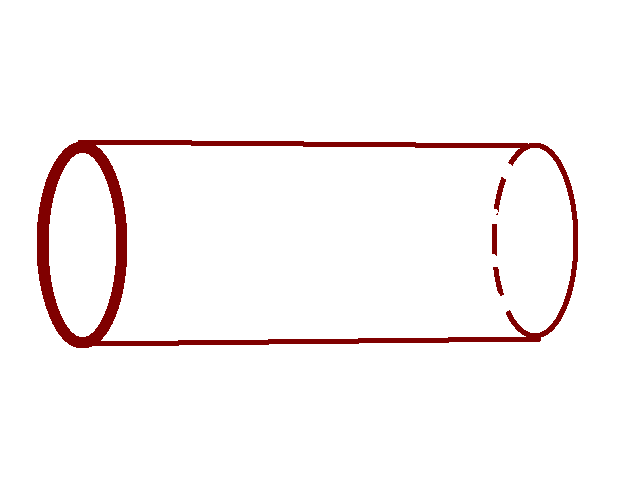
\includegraphics[width=2.5in]{Cylindrical4.png}
 \end{center}
\caption{\small 一个半无限长圆柱，左端带有一个边界。\figloc{27}{42}}
 \label{Cylindrical4}
\end{figure}
现在让我们考虑一个仅仅{\it 半}无限长的圆柱，譬如说左端带有一个边界（图 \ref{Cylindrical4}）。
与之前相同的参数 $\alpha$ 仍有意义，我们仍可把它绝热地增加 $2\pi$。
由于量子霍尔系统是有能隙的，如果在远离边界处作测量，
我们仍会看到与之前相同的价电子向左的通量，这假定了只有价带（费米能以下的状态）被填充。

% [Tutor Note: 易错——此处的“边缘态”指沿边界（半无限圆柱左端的圆周）传播的一维模，而净电荷输运沿圆柱轴向；$\veps$-$p$ 平面（图 \ref{HalfBands}）中的“向上流动”是能量方向的谱流，“每周期输运一个单位电荷”由 $\alpha\to\alpha+2\pi$ 的周期决定。两个方向不要混淆。]
但是，当电子到达左端边界时会发生什么？部分答案是：存在边缘态，电子从价带进入边缘态。
但这还不够：由于边界长度有限，只有有限多个电子能够进入（能量合理的）边缘态。
至少在一个拓扑能带绝缘体中（能带数有限，因而电子的可能能量有上界），实际发生的是：
当电子从价带（体内通常 $\veps_F$ 以下的能带）向左流入时，它们最终必须从导带（通常 $\veps_F$
以上的能带）向右流回。此外，这一切在能量上是连续发生的，
因此电子必须能够从体内的价带{\it 连续地}演化到体内的导带，并以某种方式经过边缘态。

% [Tutor Note: 笔误——图 \ref{HalfBands} 的图注（原文 Figure 28）中 “the edge-localized state becomes indistinguishable form a bulk state” 的 “form” 疑为 “from” 之误；译文按 “from”（与体态不可区分）处理。]
   \begin{figure}
 \begin{center}
   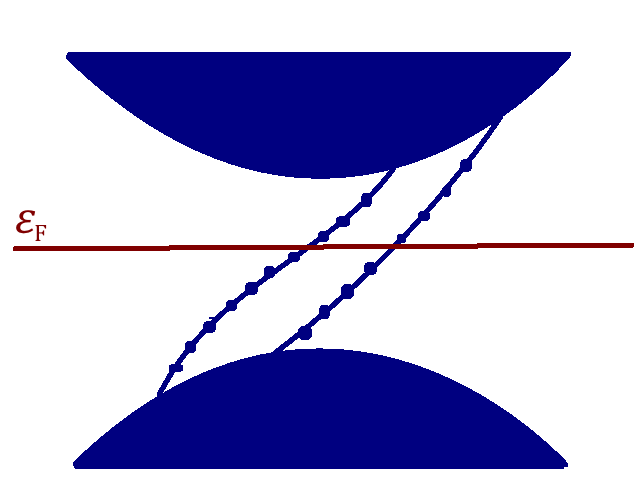
\includegraphics[width=3in]{HalfBands2.png}
 \end{center}
\caption{\small 这里画出的是 $\veps-p$ 平面，其中 $\veps$ 是电子能量，$p$
是电子沿量子霍尔区域边界方向的动量。实心区域是价带与导带投影到 $\veps-p$ 平面上的像。
（在这些投影中，电子动量垂直于边界的分量被遗忘了，因为它在边界附近不是守恒量。）
图中的每一条曲线代表一个右行边缘模，它把体价带的投影与体导带的投影连接起来。
（在所画的情形中，有两条这样的曲线，对应于 $k=2$。）
这样一条曲线代表一族边缘局域态的能量-动量关系；正如第一讲关于费米弧的讨论，
该曲线终止于这样一点：在那里边缘局域化失效，边缘局域态变得与体态不可区分。小圆珠表示：对参数
$\alpha$ 的某个取值，当边界周长 $S$ 有限时，边缘态边界动量的允许取值。\figloc{28}{43}}
  \label{HalfBands}
\end{figure}

 \subsection{连接价带与导带}

因此能谱必定看起来大致如图 \ref{HalfBands} 所示：必定存在边缘局域态，
它们能够连续地离开价带、向上流过费米能，并最终并入导带。在圆柱的周长 $S$ 趋于无穷的极限下，
边缘局域态具有连续谱；但对有限的 $S$，它们具有离散谱，如图所示。图中每一条位于 $\veps-p$
平面内、连接价带与导带的曲线都代表一个右行边缘模。曲线上的小圆珠代表当 $S$
取某个大值时曲线上允许的取值点。当我们绝热地增加 $\alpha$ 时，每个小圆珠沿曲线向上移动；在
$\alpha\to \alpha+2\pi$ 下，每个圆珠都移到下一个圆珠的位置。所以在 $\alpha\to \alpha+2\pi$
下，对每一个右行边缘模，都有净电荷 1 从价带流向导带。

% [Tutor Note: 易错——式 \eqref{trof} 的 $k=n_+-n_-$ 把边缘态计数与体霍尔电导率系数等同起来，这是反常流入（anomaly inflow）的定量表述：体态的 CS 项在边界上要求恰好 $k$ 个净手征边缘模。注意 $n_\pm$ 是计入能带简并后跨过 $\veps_F$ 的分支数；这里 $k$ 与 2.3 节 CS 系数 $k$（霍尔电导率 $k/2\pi$）是同一个量。若把 $\alpha$ 的绕行方向或 $\epsilon^{012}$ 的定向反转，则 $n_+\leftrightarrow n_-$ 而 $k\to-k$，式 \eqref{trof} 不变。]
回想我们第一讲中的讨论：一维模是右行的，只要在 $\veps=\veps_F$ 处有 $\d\veps/\d p>0$。
左行模在 $\veps=\veps_F$ 处有 $\d\veps/\d p<0$，并且在 $\alpha\to \alpha+2\pi$
下产生从价带到导带的净电荷流 $-1$。因此，若以 $n_+$ 和 $n_-$ 分别表示右行模与左行模的数目，
则在 $\alpha\to\alpha+2\pi$ 下的净电荷流为
 \be\label{trof}k=n_+-n_-.\ee

% [Tutor Note: 含糊——“端点处边缘态不再可归一化”一句省略了实质论证：边缘局域态的横向衰减长度在端点 $p_\pm$ 处发散，其波函数在 $\veps$-$p$ 平面上的投影与体态重合，因而无法再区分。这与第一讲关于费米弧端点的论证（图 \ref{twoob} 及相应的半空间边界条件）是同一机制，可用第一讲的模型哈密顿量直接验证。]
这个解释中还有一些松散的环节需要交代清楚。
一维边缘模不可能定义在边界的一维布里渊区（它是一个圆）的整体上，
因为否则我们就会受制于这样一个事实：在周期性轨道上“有上必有下”，从而得到 $n_+=n_-$。
这种不对称来自这样一些边缘模分支：它们只存在于有限的动量范围 $p_-\leq p\leq p_+$ 内。
在端点处发生了什么？答案与昨天讨论的颇为相似的费米弧例子相同。
一族边缘局域态之所以会在某个动量处不复存在，是因为它不再可归一化。
这发生在边缘态变得与体态不可区分之时。

这正是使绝热输运能够通过边缘态、从价带（通常被填充的状态）进行到导带（通常为空的状态）
的部分原因。在边缘态能谱的端点处，边缘态与体态不可区分。

% [Tutor Note: 易错——$\Tr\F+\Tr\F'=0$ 是对能带指标求迹后的恒等式（在光滑标架下逐点成立），并不意味着每条能带的贝里曲率都为零：占据带与空带的投影算符合起来是全空间的恒等投影，故 $\Tr\A+\Tr\A'$ 为全微分。单条能带的 $\Tr\F$ 一般不为零，正是它与 $\Tr\F'$ 的差别给出霍尔电导率；式 \eqref{twobbb} 的两个积分都取在同一个布里渊区 $B$ 上。$\Tr\F'=-\Tr\F$ 意味着空带的霍尔电导率恰为填充带的相反数，这是下文“流入边界与流出边界的电子数相等”的关键。]
要使这一切自洽，绝热输运必须在导带中从边界移走的电子数，等于在价带中抵达边界的电子数。
换言之，空的（导）带的总霍尔电导率必须等于填充的（价）带的霍尔电导率的相反数。
这实际上是贝里联络的一个性质。设 $\A$ 为填充能带的通常贝里联络，$\F$ 为相应的曲率；类似地，
设 $\A'$ 与 $\F'$ 为空能带的贝里联络与曲率。则 $\Tr\,\F+\Tr\,\F'=0$，
根本原因是把所有能带合在一起看时没有贝里曲率。（这个和 $(\Tr\,\F+\Tr\,\F')/2\pi$
将代表所有能带合在一起的第一陈类，而它为零，
因为所有电子态合在一起构成布里渊区上的一个平凡向量丛。）

确实，填充能带与空能带的霍尔电导率分别为
 \be\label{twobbb}\int_B\frac{\Tr \,\F}{2\pi},~~~~\int_B\frac{\Tr\,\F'}{2\pi}.\ee
因此关系式 $\Tr\,\F+\Tr\,\F'=0$ 意味着导带与价带具有相反的霍尔电导率；而在我们的思想实验中，
“填充”态（即在无限长圆柱的基态中会被填充的状态）向左的流动，等于“空”态向右的流动。

 \subsection{再论分数量子霍尔效应}\label{moref}

接下来我想解释这样一个论断：分数量子霍尔系统在 $\alpha\to \alpha+2\pi$
下并不回到它先前的状态。我们将沿用之前用过的分数量子霍尔系统的宏观模型，它以电磁矢量势 $A$
和一个只存在于材料内部的演生 $U(1)$ 规范场 $a$ 来描述：
 $$I_\eff=\frac{1}{2\pi}\int_{M_3}\d^3x\,\,\epsilon^{ijk}A_i\partial_j a_k -\frac{r}{4\pi}\int_{M_3}\d^3x\,\,\epsilon^{ijk}a_i\partial_j a_k . $$ 
如图 \ref{Cylinder} 那样，我们考虑一个圆柱形样品，并定义 $\alpha=\oint_\gamma A$。
首先让我们讨论对于给定的 $\alpha$ 如何刻画系统的状态。

原则上，$\alpha=\oint_\gamma A$ 可以通过改变穿过圆柱的磁通量来控制。但还存在一个类似的参数
$\hat\alpha=\oint_\gamma a$，它不能以这种方式控制。与 $\alpha$ 一样，$\hat\alpha$ 只在模
$2\pi$ 的意义下具有规范不变性。

关于 $\hat\alpha$ 我们能说什么？回忆 $F=\d A$、$f=\d a$ 分别是通常的电磁场强及其对 $a$
的类似物，该系统的经典场方程为
 \be\label{classeq}rf=F.\ee
在无限长圆柱的极限下，$a$ 可以按经典场处理。（更有意思的有限长圆柱情形留到第三讲。）在规范
$A_0=a_0=0$ 下，方程 $rf_{0i}=F_{0i}$ 变为
 $$r\frac{\d a_i }{\d t}=\frac{\d A_i}{\d t},$$
因此
 $$r\frac{\d\hat\alpha}{\d t}=\frac{\d\alpha}{\d t}.$$

% [Tutor Note: 笔误——原文 “the Hall conductivity can be smaller than its usual ``quantum'' by a factor of $r$” 中 “quantum” 后疑脱 “value”（通常的量子化值）；即 $\sigma_{xy}$ 可以是通常量子值 $1/2\pi$ 的 $1/r$ 倍。]
% [Tutor Note: 易错——$\alpha\to\alpha+2\pi r$ 的周期性与 $\hat\alpha$ 的 $2\pi$ 周期性是同一件事：在 $A_0=a_0=0$ 规范下由式 \eqref{classeq} 得 $r\hat\alpha=\alpha+{\rm const}$。分数霍尔电导率要求 $r$ 为整数，否则 $a$ 的大规范变换不能闭合，$\hat\alpha$ 的量子化与准粒子的分数电荷都会失去自洽性。]
所以，当我们把 $\alpha$ 绝热地增加 $2\pi$ 时，$\hat\alpha$ 绝热地增加 $2\pi/r$。由于
$\hat\alpha$ 只在模 $2\pi$ 的意义下规范不变，平移 $\hat\alpha\to\hat\alpha+2\pi/r$
并不使系统回到原来的状态。我们需要取 $\alpha\to \alpha+2\pi r$，
因此霍尔电导率是通常量子化值的 $r$ 分之一（即比通常的量子化值小 $r$ 倍）。

图\ref{HalfBands}仍有某种类似物，但边缘态不可能是自由电子态：它们必须能够在
$\alpha\to\alpha+2\pi$ 下输运分数电荷，并且只在 $\alpha\to\alpha+2\pi r$
下才回到它们原来的状态。

 \subsection{再论费米弧}

最后，我们将再次考察第一讲中讨论过的费米弧。在第一讲中，
我们考虑了一个在一般能带交叉点附近成立的模型哈密顿量，并作了显式计算以展示边缘局域态的出现。
然而，预言这些态的最初论文 \cite{WTVS} 并不是通过求解一个模型薛定谔（Schr\"odinger）
方程来进行的。相反，结果是由我们今天已解释的一些内容按如下方式推导出来的。

首先回忆基本设置。外尔（Weyl）点出现在布里渊区中价带与导带相交的特殊点处（图 \ref{twoob}）。
在有限样品的边界附近，三个动量分量中只有两个守恒。因此，把布里渊区及其中的坏点投影到二维（图
\ref{projection}）、“忘掉”不守恒的那个动量分量，是有用的做法。重要的是要记住：在晶体中，
动量分量（包括正在被“忘掉”的那个分量）都是周期的；特别地，图中的水平方向代表一个圆
$U\cong S^1$，尽管这一点很难画出来。

     \begin{figure}
 \begin{center}
   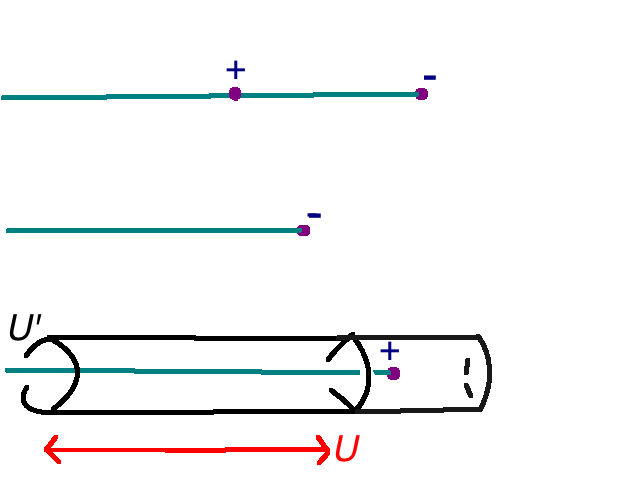
\includegraphics[width=2.5in]{Special3.png}
 \end{center}
\caption{\small 体布里渊区到适用于边缘态的边界布里渊区的投影。在投影中，
电子动量垂直于边界的分量（这里水平画出）被遗忘了。该分量由圆 $U$ 参数化。
图中我们还围绕体内部一个能带交叉点的投影画了另一个圆 $U'$。乘积 $U\times U'$
是一个二维环面。这个二维环面被用作一个辅助量子霍尔系统的布里渊区，该系统可用于分析费米弧。\figloc{29}{46}}
  \label{Special3}
\end{figure}
现在，如图 \ref{Special3} 所示，在其中一个坏点的投影周围画一个小圆 $U'$。乘积 $U\times U'$
是一个二维环面。我们定义整数 $k^*$ 为穿过 $U\times U'$ 的贝里通量：
      $$k^*=\int_{U\times U'}\d^2 p \,\frac{\Tr\,\F}{2\pi}. $$
这个整数对 $U\times U'$ 所包围的每一个正外尔点或负外尔点贡献 $1$ 或 $-1$。因此在所画的例子中
$k^*=1$；但若取 $U'$ 包围图 \ref{Special3} 投影中另外两个特殊点之一，就会得到 $k^*=0$ 或
$k^*=-1$。

我们已经作了安排，使二维环面 $U\times U'$ 不与任何外尔点相交。于是，限制到 $U\times U'$ 上，
三维布里渊区 $B$ 上原来的三维能带哈密顿量给出一个由二维环面 $U\times U'$
参数化的有能隙哈密顿量 $H^*$。我们可以把 $H^*$ 解释为某个二维晶格系统的能带哈密顿量，
该系统的霍尔电导率为 $k^*$。因此，正如我们已经学到的，$H^*$ 具有数目等于 $k^*$ 的边缘模，
它们在能量上“桥接”填充能带与空能带之间的能隙。这一点示意于图 \ref{Special4}。

        \begin{figure}
 \begin{center}
   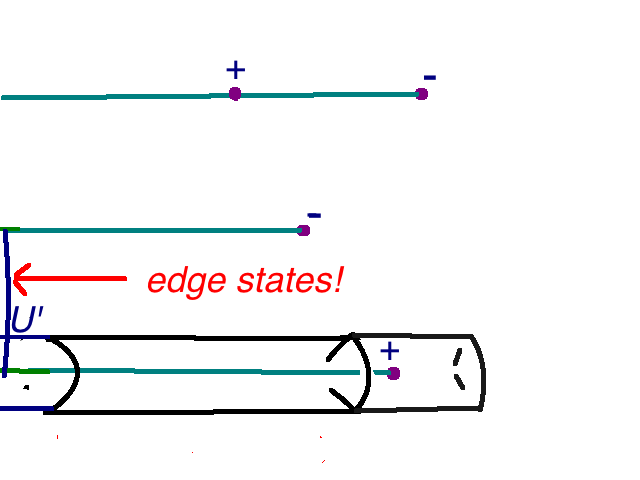
\includegraphics[width=2.5in]{Special4.png}
 \end{center}
\caption{\small $U\times U'$ 上的能带拓扑使得必定存在边缘态，它们与圆 $U'$ 相交，
并把边界布里渊区中那些具有非零净手征性的体能带交叉点的投影点连接起来。\figloc{30}{47}}
  \label{Special4}
\end{figure}

因此必定存在与 $U'$ 相交的边缘态（边缘态不是由 $U$ 标记的，因为 $U$
参数化的是与边缘态无关的动量分量）。由于我们在选择 $U'$ 时有很多自由，
边缘局域态的能谱必须由一些弧组成，这些弧把能带交叉点的投影连接起来。

这个论证中所用的辅助二维量子霍尔系统，据我所知，
与我们正在研究的三维外尔半金属之间并没有任何简单的关系。


\section{第三讲}

\begin{keytakeaways}
  \item 分数量子霍尔相的宏观模型：电磁矢量势与只存在于材料内部的演生 $U(1)$
        规范场通过混合陈-西蒙斯作用量耦合；对演生规范场带荷的准粒子携带普通的分数电荷，
        其大小由陈-西蒙斯能级 $r$ 决定。
  \item 磁单极子思想实验表明：只要霍尔电导率系数不是整数，
        样品中就必须存在带分数电荷的准粒子。
  \item 把演生规范场作量子化处理后，纯陈-西蒙斯理论是无度规的拓扑量子场论；
        它没有局域激发，只描述基态的动力学与准粒子的拓扑性质。
  \item 在环面上，能级为 $r$ 的 $U(1)$ 陈-西蒙斯理论给出 $r$
        个简并基态；威尔逊圈算符的代数关系（式 \eqref{woof}）要求 $r$ 维不可约表示，
        这是拓扑简并的最简单实例。
  \item 真空简并只在热力学极限下严格成立；
        准粒子绕不可收缩圈隧穿会以指数小的效应解除简并。
  \item 本讲随后将通过耦合有质量狄拉克费米子的方法重新解释整数量子霍尔效应中的边缘态，
        并介绍霍尔丹的无需外加磁场的量子霍尔模型。
\end{keytakeaways}

今天的讲座将涉及三个主题：（1）再论分数量子霍尔效应；（2）
对整数量子霍尔效应中边缘态的另一种解释；（3）霍尔丹（Haldane）
的无需外加磁场的量子霍尔物理模型 \cite{Haldane}。

\subsection{再论分数量子霍尔效应}

% [Tutor Note: 易错——式 \eqref{welf} 的归一化：$A\,da$ 项系数 $1/2\pi$、$a\,da$ 项系数 $-r/4\pi$，由此 $rf=F$；消去 $a$ 后得 $I'_{\rm eff}=\frac{1}{4\pi r}\int A\,dA$，即霍尔电导率为通常量子值 $1/2\pi$ 的 $1/r$（对照 2.1--2.3 节 $I=\frac{k}{4\pi}\int A\,dA$ 给出 $k/2\pi$）。注意这里只写了 $A$ 的麦克斯韦项而 $a$ 没有麦克斯韦项，这是低能有效理论的关键假定：$a$ 的动能被 $r$ 阶陈-西蒙斯项压制。另 $M_2$ 为二维空间面，$M_2\times\RR$ 即材料所在的 $2+1$ 维时空。]
与昨天一样，我们用一个有效作用量从宏观上描述分数量子霍尔系统，其变量是电磁矢量势 $A$
和一个只存在于分数量子霍尔材料内部的“演生” $U(1)$ 矢量势 $a$。
我们可以把有效作用量取为体麦克斯韦（Maxwell）作用量
\be\label{delf}\frac{1}{2e^2}\int_{\RR^{3,1}}\d^3x\d t\,\left(\vec E^2-\vec B^2\right)\ee
与一个“生活”在材料中的项之和：
\be\label{welf}I_\eff=\int_{M_2\times \RR}\d^2x\d t\,\left(\frac{1}{2\pi}\epsilon^{ijk}A_i\partial_j a_k -\frac{r}{4\pi}\epsilon^{ijk}a_i\partial_j a_k\right) . \ee



% [Tutor Note: 易错——$q$ 是准粒子对 $a$ 的荷，必须是整数：$a$ 是紧致 $U(1)$ 规范场，大规范变换要求 $e^{iq\oint a}$ 单值。其普通电荷 $q/r$ 完全由 $A$--$a$ 混合陈-西蒙斯项感生，故“分数电荷”并不破坏电荷守恒。核对式 \eqref{pelf} 时注意 $a_0$ 在 $\epsilon^{ijk}a_i\partial_ja_k$ 中以 $i=0$ 与 $k=0$ 两种方式出现，分部积分后各贡献一半，合起来才是 $-rf_{12}/2\pi$；漏掉因子 2 会得到相差一倍的分数电荷。]
为了先有个初步印象，让我们考虑一个对 $a$ 带荷 $q$ 的“准粒子”应如何解释。这里 $q$
必须是整数，因为 $a$ 是一个 $U(1)$ 规范场。若这样的准粒子静止地存在于 $M_2$ 中的一点
$x=x_0$，那么作用量中依赖于 $a$ 的部分会多出一项，成为
\be\label{melf}\int_{M_2\times \RR}\d^2x\d t\,\left(\frac{1}{2\pi}\epsilon^{ijk}A_i\partial_j a_k -\frac{r}{4\pi}\epsilon^{ijk}a_i\partial_j a_k\right) +q\int\d t
\,a_0(x_0,t). \ee
$a_0$ 的场方程变为
\be\label{pelf}\frac{F_{12}(x)}{2\pi}-\frac{rf_{12}(x)}{2\pi} +q\delta(x-x_0)=0.\ee

为了解这个方程，我们显然需要在 $F_{12}$ 和（或）$f_{12}$ 中含有德尔塔函数。
但究竟是在哪一个之中？在凝聚态物理中，$f$ 或 $F$
中的德尔塔函数实际上是对一根极细通量管的理想化。由于 $a$ 与 $f$ 只存在于二维空间中，$f$
中的德尔塔函数是合理的。它代表支撑在二维曲面 $M_2$ 上点 $x_0$ 附近的一根小通量管（图
\ref{Deltao}）。德尔塔函数的系数决定了 $f$ 在 $M_2$ 上的积分。
  \begin{figure}
 \begin{center}
   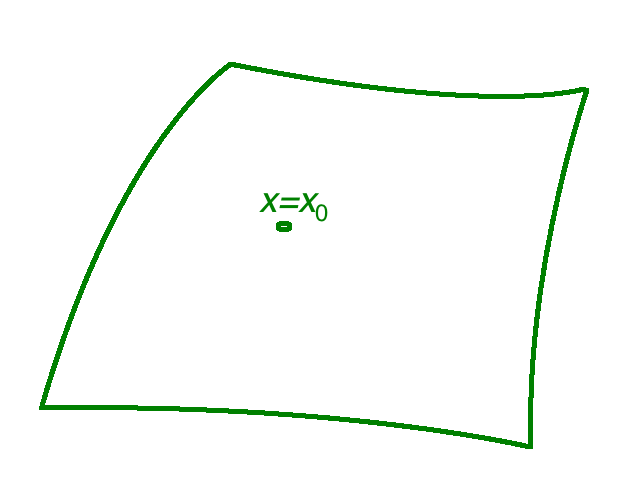
\includegraphics[width=2.5in]{Delta.png}
 \end{center}
\caption{\small 二维曲面中 $f$ 的一根通量管。$f$ 除在点 $x=x_0$ 附近极小邻域外为零，
且具有非零的积分。\figloc{31}{48}}
 \label{Deltao}
\end{figure}

% [Tutor Note: 易错——$f$ 与 $F$ 的定义域不同是本节论证的支点：$a$、$f$ 只在二维面 $M_2$ 上有定义，故 $f$ 中的点状（德尔塔函数）通量管是允许的；$A$、$F$ 定义在整个 $3+1$ 维时空，磁通管必须沿第三维延展，故 $F_{12}$ 中不可能有点源。这正是“准粒子只对 $a$ 荷化、其电磁荷是感生的”之几何来源。]
由于 $A$ 存在于整个 $3+1$ 维时空中，这样的德尔塔函数对 $F=\d A$ 并不合理。当然，
我们可以设想一根细螺线管产生 $F$ 的通量管，但它会延伸到第三个空间维度中去。
它不能代表一个位于 $M_2$ 中的准粒子。另一种做法是考虑 $M_2$ 中一个小的电流回路，譬如说半径
$\rho$ 很小。这样的电流回路会在 $3+1$ 维中产生一个磁偶极场。偶极的磁力线构成闭合回路，穿过
$M_2$ 的净通量为零：若 $F$ 是电流回路的偶极磁场，则 $\int_{M_2}F=0$。（无论电流回路是否位于
$M_2$ 中，这一点都成立。）因此在粗粒化之后，一个小的电流回路给出的是 0，而不是 $F$
中的德尔塔函数。

所以我们必须在 $f_{12}$ 中、而不是在 $F_{12}$ 中取德尔塔函数，来解方程
 \be\label{lof}\frac{F_{12}(x)}{2\pi}-\frac{rf_{12}(x)}{2\pi} +q\delta(x-x_0)=0\ee
于是在 $x=x_0$ 附近，
 \be\label{qof}\frac{f_{12}(x)}{2\pi}=\frac{q}{r}\delta(x-x_0).\ee
% [Tutor Note: 笔误——式 \eqref{meff} 中第二项写作 $\int_{M_2\times\RR}\d^3x$，而第一项与式 \eqref{welf} 均写作 $\int_{M_2\times\RR}\d^2x\d t$；$M_2\times\RR$ 本是三维，两式指同一测度，疑为记号未统一（照译不改，核对时可把它读作 $\d^2x\,\d t$）。]
现在，若回到作用量
 \be\label{meff}I_\eff=\frac{1}{2\pi}\int_{M_2\times \RR}\d^2x\d t\,\,\epsilon^{ijk}A_i\partial_j a_k -\frac{r}{4\pi}\int_{M_2\times\RR}\d^3x\,\,\epsilon^{ijk}a_i\partial_j a_k ,\ee
便看到 $A$ 的电荷密度 $J_0=\delta I_\eff/\delta A_0$ 为
 \be\label{pefr}J_0=\frac{f_{12}}{2\pi}=\frac{q}{r} \delta(x-x_0).\ee
因此，一个对 $a$ 带荷 $q$ 的准粒子具有普通的电荷 $q/r$（以电子电荷为单位）。


其实，要看出分数量子霍尔系统必然具有带分数电荷的准粒子，并不需要如此详细的计算。
让我们暂时回到整数量子霍尔系统：
 \be\label{tfor}I_\eff=\frac{k}{4\pi}\int \d^2x \d t \,\epsilon^{ijk}A_i\partial_j A_k,~~~k\in \Z.\ee
相应的电荷密度为
\be\label{dfor}J_0=\frac{\delta I_\eff}{\delta A_0}=\frac{kF_{12}}{2\pi}.\ee 

  \begin{figure}
 \begin{center}
   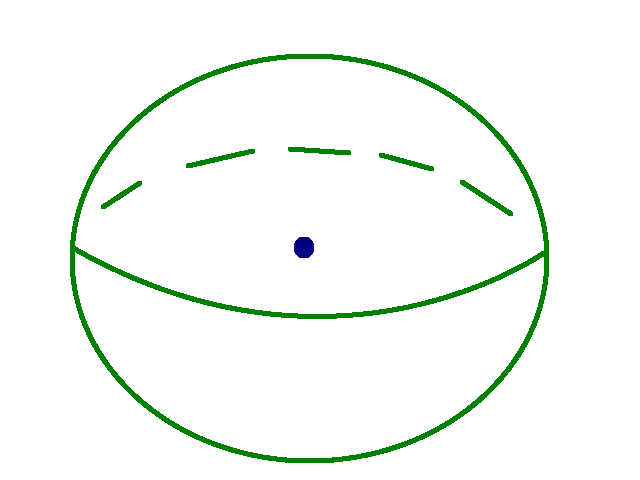
\includegraphics[width=2.5in]{Monopole.png}
 \end{center}
\caption{\small 一个内部含有磁单极子的球形量子霍尔样品。陈-西蒙斯有效作用量预言：
若不存在准粒子，则量子霍尔样品中被感生的电荷将等于 $k$，即霍尔电导率的系数。若 $k$ 为整数，
系统可以处处接近其基态；但若 $k$ 为分数，则带分数电荷的准粒子必然存在。\figloc{32}{49}}\label{Monopole}
\end{figure}

% [Tutor Note: 含糊——“$k$ 非整数则必有分数电荷准粒子”的论证隐含两个前提：(i) 孤立磁单极子的磁通为狄拉克通量量子（狄拉克通量量子化条件），(ii) 样品总电荷为整数，且把样品从无穷远处“包”到单极子周围时电荷守恒、真空为绝缘体。这是 Laughlin 磁通量子化论证的拓扑版本；拓扑序与准粒子分数的系统讨论见 \cite{Wen}。]
如果我们把一个带有一个狄拉克通量量子的磁单极子
\be\label{groof}\int \frac{F_{12}}{2\pi}=1\ee
放在球形样品内部（图 \ref{Monopole}），那么陈-西蒙斯有效作用量预言，这会在材料中感生电荷
 \be\label{droof}Q=\int_{M_2}  J_0=\int_{M_2} \frac{kF_{12}}{2\pi}=k,\ee
只要 $k$ 是整数，一切就都正常。但若 $k$
的有效值不是整数——分数量子霍尔效应就是这种情况——那么电荷必定还有额外的贡献，
其形式是出现在材料表面某处的带分数电荷的准粒子。的确，考虑如下思想实验：
开始时真空中有一个孤立的磁单极子。然后我们从无穷远处取来大量但有限多的原子，
把它们组装成一个包围该磁单极子的大球形分数量子霍尔系统，如图所示。
我们可以做到让原子始终远离单极子。由于电荷守恒且真空是绝缘体，单极子的电荷在此过程中不变。
包围单极子的球形量子霍尔样品的总电荷必为整数，因为这个系统归根到底由有限多个电子、
质子和中子组成，而它们每一个的电荷都是整数。然而系统的总电荷将是式 (\ref{droof}) 的“体”贡献
$k$ 与可能存在的任何准粒子的进一步贡献之和。若 $k$ 不是整数，
那么包围磁单极子的球形量子霍尔系统就必定含有带分数电荷的准粒子。


要完整理解分数量子霍尔系统，需要把 $a$ 作量子力学处理。本讲不试图给出完整的解释，
只解释几个基本要点。

% [Tutor Note: 术语——“topological quantum field theory”（拓扑量子场论）在此有确定含义：作用量中不出现度规，故理论对时空度规不敏感，只有整体（拓扑）自由度被量子化，Hilbert 空间有限维、无局域激发。注意它与“拓扑能带理论”（第一讲对自由费米子的讨论）层次不同：这里的 TQFT 是强关联 FQHE 的低能有效描述。又，下文“不存在局部规范不变可观测量”亦应如此理解：局部多项式只能由 $f$ 构造，而在壳 $f=0$，故 $\HH$ 只能由 Wilson 圈构造。]
首先，我们之所以能在未对 $a$ 作量子力学处理的情况下走到这一步，
部分原因是我们迄今考虑的是无限长或半无限长圆柱（如图 \ref{Cylindrical4} 所示）
上的分数量子霍尔系统；在这种情形下，许多问题并不需要完整的量子处理。例如，在 \ref{moref}
节中，我们把 $\hat\alpha=\oint_\gamma a$ 当作任意常数，而不是量子变量。
这在无限长或半无限长圆柱上是可行的；但对于紧致样品，我们确需把 $a$ 作量子力学处理。

在讨论 $a$ 的量子力学时，我们将忽略 $A$，只研究纯粹的 $2+1$ 维问题：
 \be\label{loof}I_\eff=-\frac{r}{4\pi}\int_{M_2\times\RR}\d^3x\,\,\epsilon^{ijk}a_i\partial_j a_k . \ee
一个值得注意的事实是，{\it 这里根本看不到度规张量}，因此我们要描述的是一个“拓扑量子场论”。
它将不描述粒子激发，而只描述“基态的动力学”以及准粒子的拓扑性质。在长距离下，
许多乃至大多数有能隙的量子系统直接变得平庸，
我们通常把这一点视为有能隙系统长距离行为的理所当然。但更一般地，
一个有能隙的量子系统在长距离下可以导致非平庸的拓扑量子场论；分数量子霍尔效应就是如此。

   \begin{figure}
 \begin{center}
   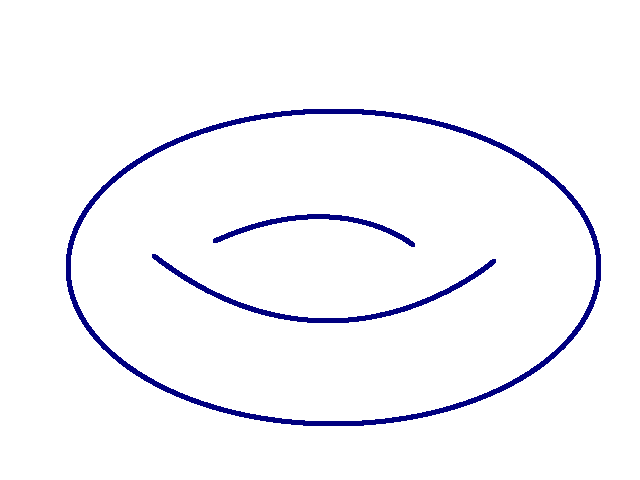
\includegraphics[width=2.5in]{Torus.png}
 \end{center}
\caption{\small 一个二维环面。\figloc{33}{50}}
  \label{Torus}
\end{figure}
具有非平庸拓扑的紧致样品——例如图 \ref{Torus} 中的环面——尤其令人感兴趣。我们要找出场 $a$
在这样的流形上量子化后的量子态。


这些量子态应当构成一个希尔伯特空间 $\HH$。$\HH$ 应当给出某个量子算符代数的表示，
而这个代数在某种意义上是通过把经典可观测量的空间量子化得到的。在规范场论中，
我们只考虑规范不变的经典可观测量。因此我们应当问：“由 $a$ 能造出哪些规范不变的经典可观测量？”
一旦提出这个问题，我们就会遇到如下事实。一个规范不变的局部算符必须是 $f=\d a$
及其导数的多项式。但 $a$ 的经典场方程是
 \be\label{doof}f=0,\ee
因此不存在局部、规范不变的经典可观测量。

% [Tutor Note: 易错——式 \eqref{ooff} 中 $s\in\Z$：荷量子化使 Wilson 圈只能携带整数荷，相位 $e^{is\oint a}$ 在大规范变换 $\oint a\to\oint a+2\pi$ 下不变。注意指数中没有 $1/2\pi$，而式 \eqref{welf} 中 $a$ 的归一化含 $1/2\pi$；两者配合才决定准粒子荷 $q=s$ 与分数电荷 $s/r$ 的对应关系，核对时不要漏掉 $a$ 的归一化。]
然而，确实存在规范不变的“威尔逊圈”算符。我们取一条闭曲线 $\ell\subset M$，
并定义“威尔逊圈算符”
 \be\label{ooff}W_s(\ell)=\exp\left(is\oint_\ell a\right),~~~s\in \Z.\ee
该算符在 $\ell$ 的连续形变下不变。这里有两个相关的解释：（a）这是因为 $f=0$，所以
$W_s(\ell)$ 只能“看到”诸如阿哈罗诺夫-玻姆（Aharonov-Bohm）相位那样的整体信息；（b）
更一般地，在任何拓扑量子场论中，微分同胚都是对称性，任何圈 $\ell$ 都通过微分同胚等价于
$\ell$ 所能形变到的任何邻近圈。


威尔逊圈算符 $W_s(\ell)$ 的物理意义是：一个电荷为 $s$ 的准粒子绕圈 $\ell$
传播这一过程的振幅，正比于因子 $W_s(\ell)$。若圈 $\ell$
能够在没有奇点的情况下连续收缩为一点，则算符 $W_s(\ell)$ 是平庸的，因为准粒子哪里也没去。
“平庸”是指在这种情况下 $W_s(\ell)$ 作为算符等于 1。我们只关心并非如此的情形。

   \begin{figure}
 \begin{center}
   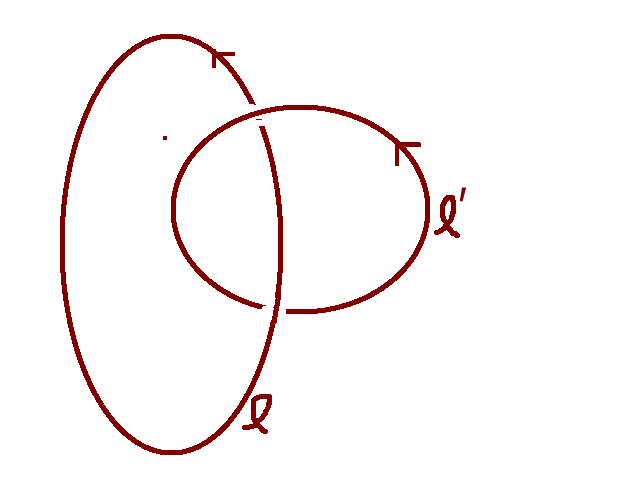
\includegraphics[width=2.5in]{Loops.png}
 \end{center}
\caption{\small $\RR^3$ 中两个圈的链接。\figloc{34}{51}}
  \label{Loops}
\end{figure}
威尔逊圈算符 $W_s(\ell)$ 可能“看到”的阿哈罗诺夫-玻姆型相位有两个可能的来源。
可能存在另一个类似算符 $W_{s'}(\ell')$，其中 $\ell$ 与 $\ell'$ “链接”在一起、无法解开（图
\ref{Loops}）。（若试图让 $\ell$ 穿过 $\ell'$，就会出现奇点。）
这种效应与准粒子的分数统计相联系：它意味着，一个准粒子沿 $\ell'$
传播的存在会改变第二个准粒子沿 $\ell$ 传播的振幅，即使两者相距很远。
另一种可能更接近经典的阿哈罗诺夫-玻姆思想：圈 $\ell$
可能由于与其他准粒子的存在无关的拓扑原因而是“不可收缩的”（图 \ref{Torus2}）。

   \begin{figure}
 \begin{center}
   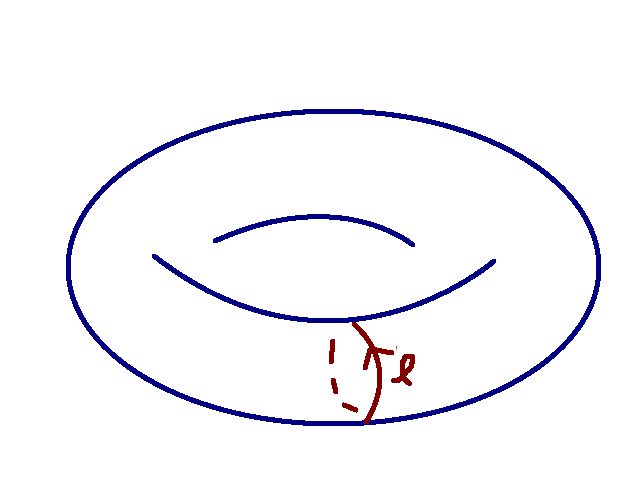
\includegraphics[width=2.5in]{Torus2.png}
 \end{center}
\caption{\small 环面上的一条不可收缩圈。\figloc{35}{52}}
  \label{Torus2}
\end{figure}

% [Tutor Note: 含糊——作者以“借助经典泊松括号或量子正则对易关系即可得知”跳过推导。实质是：由式 \eqref{loof} 得等时对易子 $[a_1(x),a_2(y)]=-(2\pi i/r)\delta^2(x-y)$（符号随 $\epsilon^{012}$ 取正序的约定），指数化后两次使用 BCH 公式即得式 \eqref{grooff}；其中相交数 $\ell\cap\ell'$ 需先固定环面定向，定向反转时指数上的相位取逆。这里必须是 $2\pi$ 而非 $4\pi$：只有 $2\pi/r$ 才能给出式 \eqref{grooff} 的 $\exp(2\pi i ss'\ell\cap\ell'/r)$；若误用 $4\pi$，相位会差一倍。]
若环面上两条这样的圈 $\ell$ 与 $\ell'$ 具有非零的相交数 $\ell\cap\ell'$（图 \ref{Torus3}），
那么——借助经典泊松括号或量子正则对易关系即可得知——相应的威尔逊算符不对易。它们满足
   \be\label{grooff}W_s(\ell) W_{s'}(\ell') =\exp(2\pi i ss'\ell\cap\ell'/r) W_{s'}(\ell')W_s(\ell).\ee

    \begin{figure}
 \begin{center}
   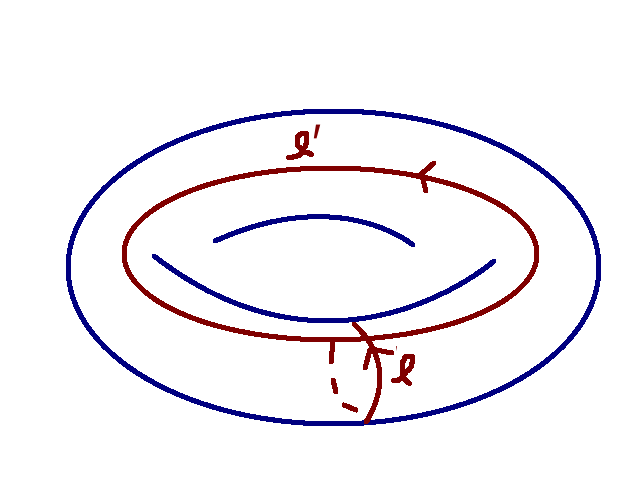
\includegraphics[width=2.5in]{Torus3.png}
 \end{center}
\caption{\small 环面上两条具有非零相交数 $\ell\cap \ell'$ 的不可收缩圈。在所画的例子中，
相交数为 1。\figloc{36}{52}}
  \label{Torus3}
\end{figure}

% [Tutor Note: 笔误——原文 “since $W_s(\ell)$ is just the $\ell^{th}$ power of $W_1(\ell)$” 中的 $\ell^{th}$ 疑为 $s^{th}$ 之误：$\ell$ 是圈，幂次应由荷给出，即 $W_s(\ell)=W_1(\ell)^s$；下文随即取 $s=s'=1$ 也印证“幂次”指的是荷。译文照原文写作 $\ell^{th}$，不改公式。]
基本情形——即图中所示——是 $\ell\cap \ell'=1$。此外，我们不妨直接取 $s=s'=1$，因为 $W_s(\ell)$
不过是 $W_1(\ell)$ 的 $\ell^{th}$ 次幂，$W_{s'}(\ell')$ 亦然。若记 $A=W_1(\ell)$、
$B=W_1(\ell')$，则 $A$ 与 $B$ 满足的代数关系为
   \be\label{woof}AB=\exp(2\pi i/r)BA.\ee
% [Tutor Note: 术语——“level”（级）在此指陈-西蒙斯作用量的系数 $r$（即 $U(1)_r$ 理论）；“不可约表示维数为 $r$”与“环面上 $r$ 个基态”是同一事实的两种说法，即拓扑简并。这里 $r$ 同时是准粒子分数电荷 $1/r$ 的分母与陈-西蒙斯能级，并非巧合：两者都由同一条陈-西蒙斯作用量的量子化决定。]
该代数的一个不可约表示具有维数 $r$，因为
   \be\label{oof}B\to ABA^{-1}=\exp(2\pi i/r)B\ee
会把 $B$ 的任一特征值乘以 $\exp(2\pi i/r)$。因此表示这个代数需要 $r$ 个态，而实际上 $r$
个态也就足够了。对于规范群为 $U(1)$、能级为 $r$ 的情形，这些就是“陈-西蒙斯理论在环面上的 $r$
个基态”。


% [Tutor Note: 易错——“真空简并”只在热力学极限下严格：有限系统上，准粒子绕不可收缩圈隧穿给有效哈密顿量加 $W_s(\ell)$ 项，其系数 $\sim e^{-mL}$（$m$ 为打开简并的能标、$L$ 为同伦类中最短圈长），使简并被指数小地解除。故拓扑简并是“指数精度”的简并而非严格简并；这一点在讨论 FQHE 的拓扑序时至关重要。]
因此，这就为如下论断提供了依据：{\it 在系统非常大的极限下}，
拓扑非平庸流形上的量子霍尔系统具有非平庸的真空简并。“在系统非常大的极限下”这一条件是必要的，
因为真空简并实际上会被指数小的效应略微解除，这些效应来自准粒子绕不可收缩圈的隧穿。电荷为 $s$
的准粒子绕图 \ref{Torus2} 所示的那种不可收缩圈 $\ell$ 的隧穿，会给有效哈密顿量贡献一项
$W_s(\ell)$，其系数指数地小。（这个系数绝对不是拓扑不变量。它依赖于准粒子的能量和圈 $\ell$
的长度——更确切地说，是其同伦类中最短圈的长度，因为那是最可能的隧穿路径。）

\subsection{再论整数量子霍尔效应的边缘态}

至此，我们对分数量子霍尔效应这一广阔主题的相当简略的介绍就结束了。
现在我们回到整数量子霍尔效应。我们大体上遵循霍尔丹（Haldane）\cite{Haldane} 的做法，
对第二讲中已熟悉的某个事实给出一个概念性的、
不作具体计算的证明（在第 \ref{tcp} 节中已给出过另一种概念性解释）：一个 $2+1$ 维系统，
若其体内具有陈-西蒙斯耦合
% [Tutor Note: 易错——式 (\ref{plof}) 的归一化为 $1/(4\pi)$；按 2.2 节的约定，$A$ 实际是通常的 $eA$（$D_i\psi=(\partial_i-iA_i)\psi$），故式中不出现 $e$。在此约定下霍尔电导率为 $k/2\pi$，即 $ke^2/h$（见 2.3 节式 (\ref{murr})）；若改用普通电磁势书写，须把 $k$ 换成 $ke^2$。]
    \be\label{plof}I_\eff=\frac{k}{4\pi}\int \d^3x\,\epsilon^{ijk}A_i\partial_j A_k, \ee
并在边界上有 $n_+-n_-=k$ 个手征边缘态，则它是完全自洽且无反常的。为说明这一点，
我们只需描述一种物理实现。我们先以连续的语言来做，然后借助霍尔丹模型来做。

我们让场 $A$ 与一个电荷为 1 的有质量 $2+1$ 维狄拉克费米子 $\psi$ 相耦合：
  \be\label{utof}I_\psi=\int \d^3x \,\bar\psi\left(\slashed{D}-m\right)\psi.\ee
由于 $\psi$ 是有能隙的，我们可以把它“积分掉”，从而得到只含 $A$ 的局域有效作用量。
结果表明，低能下的主导项是
% [Tutor Note: 易错——式 (\ref{uftof}) 的因子 $1/2$ 是宇称反常的直接体现，并非笔误：单个有质量 $2+1$ 维狄拉克费米子诱导的陈-西蒙斯系数恰为 $\pm 1/2$（以整能级为 1），故单独的 $\psi$ 理论在大规范变换下不规范不变，只有系数为整数的组合才能独立存在（参见 \cite{Red,Semenoff} 及下文式 (\ref{quft})）。此外，“低能主导项”来自对 $A$ 的导数展开：$2+1$ 维中规范不变的宇称奇项最低阶只能是陈-西蒙斯项（量纲 3），更高阶项均被 $1/m$ 的幂压低。]
  \be\label{uftof}\frac{\sign m}{2}\ICS(A)=\frac{\sign m}{2}\frac{1}{4\pi}\int\d^3x \epsilon^{ijk}A_i\partial_jA_k. \ee
$1/2$ 这个因子令人不安，因为它与规范不变性相矛盾。不过，
我们将始终考虑它不出现的那些组合。因子 $\sign m$ 来自反射对称性（在该对称性下 $m$ 与
$\ICS(A)$ 都是奇的）以及量纲分析。

    \begin{figure}
 \begin{center}
   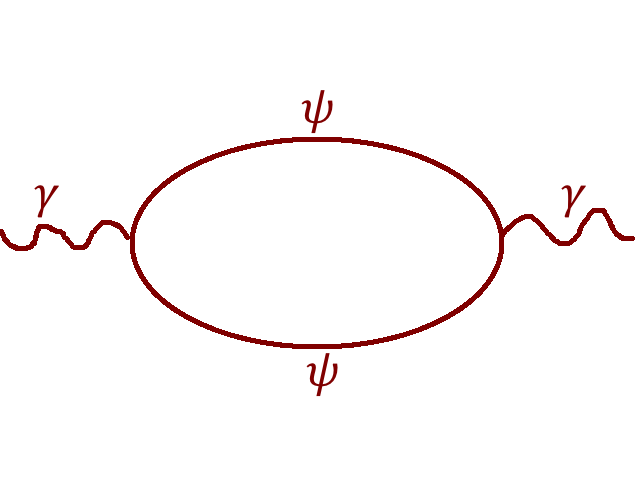
\includegraphics[width=2.5in]{Feynman.png}
 \end{center}
\caption{\small 与宇称反常相联系的单圈费曼图。\figloc{37}{54}}
 \label{Feynman}
\end{figure}

% [Tutor Note: 含糊——“这并非困难的计算”指 $2+1$ 维量子电动力学中单圈真空极化图（图 \ref{Feynman}）的计算，即真空极化张量的宇称奇部分：它有限，且正比于 $\epsilon^{\mu\nu\rho}p_\rho$，系数 $\frac12\sign m$ 不依赖正则化方案。作者略去细节，可查 \cite{Red,Semenoff}。]
有效作用量 $(\sign m/2)\ICS(A)$ 最早是由一个费曼图（图 \ref{Feynman}）得到的
\cite{Red,Semenoff}，这并非一个困难的计算。然而，本着本讲的精神，
从贝里通量出发得到这一结果更为自然。

我们知道，任何有能隙的带电费米子体系被“积分掉”之后，
所得到的 $\ICS(A)$ 的系数等于动量空间哈密顿量的缠绕数。
$2+1$ 维中的有质量狄拉克哈密顿量为
% [Tutor Note: 易错——式 (\ref{puft}) 的 $H=\sigma_xp_x+\sigma_yp_y+m\sigma_z$ 与式 (\ref{utof}) 描述同一个费米子（$2\times2$ 表示、负能带被填充）。填充能带的陈数取 $\frac12\sign m$ 还是 $-\frac12\sign m$，取决于 $\epsilon^{012}$ 的定向与 $\sigma_i$ 的符号约定；本讲取 $\epsilon^{012}=+1$，故与式 (\ref{uftof}) 的符号一致。核对时可用两式相互印证。]
\be\label{puft}H=\sigma_x p_x+\sigma_y p_y + m \sigma_z.\ee
对于大的 $|p|$，映射为
\be\label{wuft}(p_x,p_y)\to \left(\frac{p_x}{\sqrt{p_x^2+p_y^2}},\frac{p_y}{\sqrt{p_x^2+p_y^2}},0\right), \ee
它绕着球面的赤道缠绕（图 \ref{Equator}）。
   \begin{figure}
 \begin{center}
   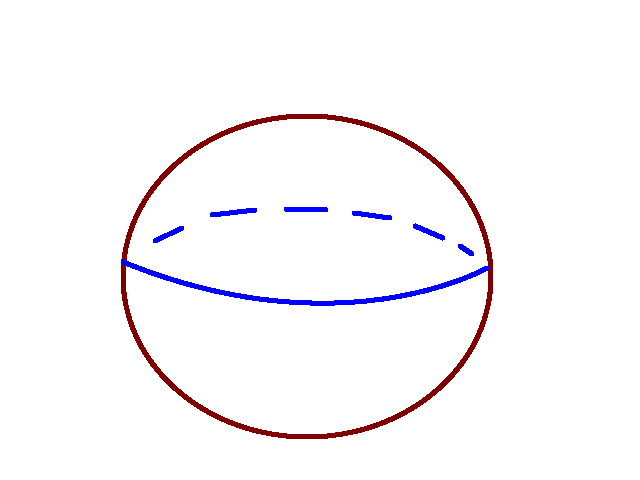
\includegraphics[width=2.5in]{Equator.png}
 \end{center}
\caption{\small 二维球面的赤道。 \figloc{38}{54}}
 \label{Equator}
\end{figure}

% [Tutor Note: 易错——“系数等于缠绕数”是 1.4 节与 2.4 节证明的结论（填充能带的贝里曲率积分给出陈数，即此处的缠绕数），作者直接引用。而“缠绕数”$\frac12\sign m$ 是半整数，这与 $\pi_2(S^2)\cong\Z$ 并不矛盾：映射 $p\mapsto(p_x,p_y,m)/\sqrt{p_x^2+p_y^2+m^2}$ 在 $|p|\to\infty$ 时趋于赤道而非一点，因而不能连续延拓为 $S^2\to S^2$ 的映射；$\frac{1}{4\pi}\int\d^2p\,\hat n\cdot(\partial_{p_x}\hat n\times\partial_{p_y}\hat n)$（$\hat n$ 为该单位向量）只覆盖半个球面。这个半整数正是宇称反常的几何来源；若在无穷远把质量取为 $+\infty$（例如加 Wilson 项）使映射紧致化，才会得到整数陈数。]
完整的映射
 \be\label{PPP}   (p_x,p_y)\to \left(\frac{p_x}{\sqrt{p_x^2+p_y^2+m^2}},\frac{p_y}{\sqrt{p_x^2+p_y^2+m^2}},\frac{m}{\sqrt{p_x^2+p_y^2+m^2}}\right)\ee
的像，依 $m$ 的符号而为上半球面或下半球面（图 \ref{Equator2}）。
因此缠绕数为 $\frac{1}{2}\sign \,m$，这正是积分掉 $\psi$ 后得到的陈-西蒙斯系数。
    \begin{figure}
 \begin{center}
   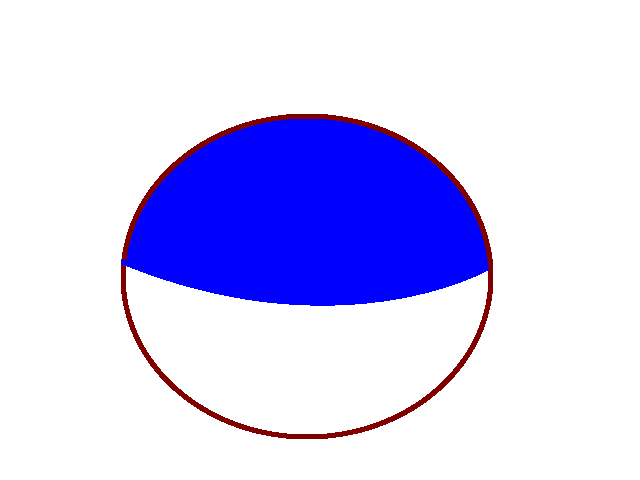
\includegraphics[width=2.5in]{Equator2.png}
 \end{center}
\caption{\small 二维球面的上半球面。\figloc{39}{55}}
 \label{Equator2}
\end{figure}

眼下，我们希望考虑一个在低能下有能隙且平庸的理论，因此除 $\psi$ 之外，
再引入一个质量为 $-m$ 的第二个费米子场 $\psi'$。这一组合之所以平庸，
是因为把 $\psi$ 与 $\psi'$ 都积分掉后所得到的总陈-西蒙斯系数为
% [Tutor Note: 易错——式 (\ref{quft}) 用到 $\sign(-m)=-\sign m$，两个费米子的贡献精确抵消；注意二者耦合到同一个 $U(1)$ 规范场 $A$，诱导的陈-西蒙斯系数按费米子数目相加。$m=0$ 处 $\sign m$ 无定义，对应能隙关闭的相变点。]
 \be\label{quft}\frac{1}{2}\left(\sign\,m+\sign\,(-m)\right)=0.\ee
没有诱导的陈-西蒙斯耦合，因此在带边界的流形上没有反常。

对于带边界的样品，我们希望选取一种边界条件，
使得系统即使沿边界也保持平庸——根本没有任何边缘激发。这当然是自洽且在物理上合理的！
那么在半空间 $x_1\geq 0$ 上，什么样的边界条件能保证沿边界不发生任何事情？

能做到这一点的边界条件是
% [Tutor Note: 易错——式 (\ref{plift}) 中的 $\gamma_1$ 是垂直于边界的伽马矩阵；在该约定下，反射 $x_1\to-x_1$ 作用在旋量上相当于左乘 $\gamma_1$，因此 (\ref{plift}) 等价于要求拼接后的 $\hat\psi$ 在 $x_1=0$ 处连续，从而 (\ref{obeys}) 成立。符号不可随意更改：若取 $\psi'=-\gamma_1\psi$，拼接处的质量项不匹配，(\ref{obeys}) 不再成立。]
 \be\label{plift}\left.\psi'\right|_{x_1=0}=\gamma_1\left.\psi\right|_{x_1=0}.\ee
回顾一下：$\psi$ 与 $\psi'$ 具有大小相等、符号相反的质量
 \be\label{ulift}\left(\slashed{\partial}-m\right)\psi=0=\left(\slashed{\partial}+m\right)\psi',\ee
并且在 $2+1$ 维中，费米子质量在反射下是奇的。因此，
若按下式把 $\psi$ 与 $\psi'$ 合并为定义在整个 $\RR^3$ 上的单个费米子 $\hat\psi$：
 \be\label{nuft}\hat\psi(x_1,x_2;t)=\begin{cases}\psi(x_1,x_2;t) & {\mathrm{if}}~x_1\geq 0 \\
                                       \gamma_1\psi'(-x_1,x_2;t) & {\mathrm{if}}~x_1\leq 0, \end{cases} \ee
那么 $\hat\psi$ 就满足
 \be\label{obeys}\left(\slashed{\partial}-m\right)\hat\psi=0,\ee
并且显然没有无能隙模。

现在，在保持费米子动能与边界条件不变的前提下，我们改变 $\psi'$ 质量的符号，
让 $\psi$ 与 $\psi'$ 都具有相同的质量 $m>0$。这不影响理论的自洽性，
因为质量是一种“软”微扰。当然，当 $\psi'$ 的质量经过零时，理论将失去能隙，
并经历一次相变。在这个相变的另一边是什么？
% [Tutor Note: 术语——原文此处把 $\ICS(A)$ 的系数直接称为“霍尔电导率”；严格说二者相差 $1/2\pi$：由 $J_2=-\delta I_\eff/\delta A_1=kF_{01}/2\pi=kE_1/2\pi$ 得 $\sigma_{xy}=k/2\pi=ke^2/h$（见 2.3 节式 (\ref{murr})）。本讲中“陈-西蒙斯系数 $k$”与“霍尔电导率 $k/2\pi$”常混用，阅读时以量纲区分。]
霍尔电导率——即有效作用量中 $\ICS(A)$ 的系数——现在是 $\frac{1}{2}\left(1+1\right)=1.$ 单
就它本身而言，这将会是反常的。但此时 $\hat\psi$ 的狄拉克方程为
      \be\label{gift}\left(\slashed{\partial}-m\,\sign(x_1)\right)\hat\psi=0,\ee
于是 $\hat\psi$ 的质量在经过 $x_1=0$ 时变号。
正如杰基夫（Jackiw）与雷比（Rebbi）\cite{JR} 的经典分析所示，
这种质量变号导致在 $x_1=0$ 附近存在一个无能隙模。
相应的解与我们已在式 (\ref{ogg}) 中见过的情形颇为相似：
% [Tutor Note: 术语——式 (\ref{trogg}) 的 $\g_1\psi_\parallel=-\psi_\parallel$ 是 $1+1$ 维意义下的手征条件：$\g_1$ 与边界上的 $1+1$ 维狄拉克算符反对易，因而充当该 $1+1$ 维理论的手征算符（相当于三维中 $\gamma_5$ 的角色）；勿与“自旋沿动量方向的投影”即螺旋度混淆。另与 1.11 节式 (\ref{ogg}) 对比：那里是半空间单侧解 $\exp(mx_1)$、$\gamma_1\psi_\parallel=+\psi_\parallel$，可归一化要求 $m<0$；此处是质量台阶上的拼合解、符号相反，二者互为镜像，核对时勿混。]
% [Tutor Note: 易错——式 (\ref{zoggg}) 的零模只在 $m>0$ 时按 $\exp(-m|x_1|)$ 指数局域、可归一化；若 $m<0$ 则发散而不能归一化。它与 (\ref{gift}) 中质量台阶 $m\,\sign(x_1)$ 的零模一一对应，是 Jackiw-Rebbi \cite{JR} 域壁零模在垂直于边界方向上的实现；注意此处的 $\psi$ 应理解为 (\ref{gift}) 中 $\hat\psi$ 的边界分量，勿与体费米子混淆。]
      \be\label{zoggg}\psi=\exp(-m|x_1|)\psi_\parallel,\ee
其中
      \be\label{trogg} \g_1\psi_\parallel =- \psi_\parallel,~~~\slashed{\partial}^\parallel\psi_\parallel=0. \ee
条件 $\g_1\psi_\parallel=-\psi_\parallel$ 使 $\psi_\parallel$ 在 $1+1$ 维意义下具有确定
的手征性；因此这样得到的，是沿 $x_1=0$ 处的边界传播的手征边缘模。

% [Tutor Note: 易错——这里每一对 $(\psi,\psi')$ 贡献 $\frac12(\sign m+\sign m)=1$ 个陈-西蒙斯能级与一个手征边缘模；$k$ 对给出 $k\ICS(A)$ 与 $k$ 个边缘模，恰满足 2.6 节的 $n_+-n_-=k$。因此无需单独验证边缘模的反常：体与边界的反常流入（2.6 节）在这里被显式配对。]
于是，我们得到了一个明显自洽的构造：一个 $2+1$ 维系统，
其在体内的有效作用量为 $\ICS(A)$（外加更高维度的项），并沿边界具有一个手征边缘模。
如果我们一开始就取 $k$ 对 $\psi,\psi'$，那么以同样的方式会得到体作用量 $k\ICS(A)$ 与 $k$
个手征边缘模。这样，我们就确认了这一组合系统的自洽性，而无需去研究手征边缘模的“反常”。

\subsection{霍尔丹的石墨烯模型}\label{hmg}

        \begin{figure}
 \begin{center}
   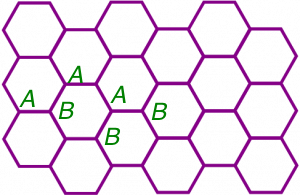
\includegraphics[width=2.5in]{Hex3.png}
 \end{center}
\caption{\small 六角（蜂窝）晶格。这是一个二分晶格：晶格格点可交替标记为 $A$ 或 $B$，
使得 $A$ 格点的最近邻皆为 $B$ 格点，反之亦然。
所有 $A$ 格点在晶格平移下彼此等价，$B$ 格点亦然。但不存在交换 $A$ 与 $B$ 格点的平移对称性。
因此，一个原胞包含一个 $A$ 格点和一个 $B$ 格点。\figloc{40}{56}}
 \label{honey}
\end{figure}

% [Tutor Note: 术语——图 \ref{honey} 所说的“二分晶格”指 $A$、$B$ 两套子晶格之间没有交换二者的平移对称性：所有 $A$ 格点在平移下等价，$B$ 格点亦然，但 $A$ 与 $B$ 不等价。每个原胞含一个 $A$ 与一个 $B$，故（不计自旋）$2p_z$ 轨道恰形成两个能带，这是后文半满讨论的前提。]
下面说明霍尔丹是如何在一个凝聚态模型中实现这一系统的——即对石墨烯标准能带哈密顿量
作一个小扰动。石墨烯是碳原子排布成六角（蜂窝）晶格的原子单层，如图 \ref{honey} 所示。
我们把它看作 $x-y$ 平面内的晶格，取 $z$ 为法向。碳原子有 6 个电子；其中 2 个处于
$1s$ 态，另外 3 个用于与任一给定原子的 3 个最近邻形成共价键。（可以认为这些键中的
电子是杂化的 $2s$、$2p_x$ 与 $2p_y$ 电子。）每个原子剩下 1 个电子，它进入 $2p_z$
轨道——自旋向上或向下。因此两个 $2p_z$ 轨道将是“半满的”。

蜂窝晶格每个原胞有两个原子。如图中所述，每个原胞含一个 $A$ 原子和一个 $B$ 原子。
因此（不计自旋） $2p_z$ 轨道形成两个能带，而我们想要把这些能带填到“半满”。

        \begin{figure}
 \begin{center}
   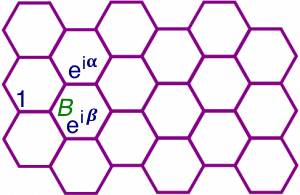
\includegraphics[width=2.5in]{Hex4.png}
 \end{center}
\caption{\small 从最近邻格点向 $B$ 格点的跃迁。\figloc{41}{57}}
 \label{honey2}
\end{figure}

% [Tutor Note: 含糊——“在某种程度上由对称性决定”指：只保留每个格点一个 $2p_z$ 轨道、最近邻跃迁振幅 $t$ 的紧束缚模型，其能带结构由晶格对称性与 $t$ 决定；更远邻的跃迁、轨道重叠等会修正色散，但不改变狄拉克点的存在性与拓扑性质。该模型见 \cite{Wallace}。]
% [Tutor Note: 易错——参数 $\alpha,\beta$ 不是三条键相位的全部：三条最近邻键各带一个相位，而整体相位可通过重新定义波函数吸收，故只有两个独立的规范不变相位；这里取其中一条键的相位为 $0$，用 $(\alpha,\beta)$ 作为二维布里渊区的坐标。]
会发生什么，在某种程度上是由对称性决定的；但理解它的最容易的办法，
是先求解一个简单模型 \cite{Wallace,Sem,GM}，
其中哈密顿量描述从 $A$ 子晶格到 $B$ 子晶格（以及反向）振幅为 $t$ 的“最近邻跃迁”。
写出动量空间哈密顿量的一个捷径如下。如图 \ref{honey2} 所示，在 $B$ 子晶格中取一点，
并令电子的动量（以及其波函数的归一化）使得三个最近邻 $A$ 点处的振幅为 $1, e^{i\alpha},$
和 $e^{i\beta}$。这里 $\alpha$ 与 $\beta$ 是任意角度；它们给出布里渊区的一种便利参数化。

于是，跃迁到所示 $B$ 格点的总振幅为 $1+e^{i\alpha}+e^{i\beta}$（再乘以跃迁常数 $t$）。
哈密顿量是厄米的，所以 $B\to A$ 的跃迁是它的复共轭；在 $A, B$ 基下，动量空间哈密顿量为
% [Tutor Note: 易错——式 (\ref{hham}) 取 $(A,B)$ 为基底、$t$ 为实数；因 $H$ 厄米，$(1,2)$ 元是 $(2,1)$ 元的复共轭，故为 $1+e^{-i\alpha}+e^{-i\beta}$。$\alpha,\beta$ 的符号约定（哪个键取 $e^{+i\alpha}$）与狄拉克点的位置有关，核对时以式 (\ref{theq}) 的零模条件为准。]
\be\label{hham}H=t\begin{pmatrix} 0  & 1+e^{-i\alpha}+e^{-i\beta}\cr 1+e^{i\alpha}+e^{i\beta}& 0\end{pmatrix}.\ee
% [Tutor Note: 笔误——原文式 (\ref{hham}) 之后另起一行单独残留一个句点“.”，系源文件的排版残留；译文未重复这个孤立句点，以免正文出现两个句号。]

$H$ 的迹为零，因此能带交叉恰好发生在 $H$ 存在零模之时。为求出这样的零模，
我们须在 $\alpha, \beta$ 为实数的条件下解
% [Tutor Note: 易错——零模条件 (\ref{theq}) 中的 $1$、$e^{i\alpha}$、$e^{i\beta}$ 是三个单位向量，三者之和为零当且仅当它们互成 $120^\circ$；因此 (\ref{omeq}) 中的 $\sqrt{-3}$ 应读作 $i\sqrt{3}$，两个解为 $e^{i\alpha}=e^{\pm2\pi i/3}$、$e^{i\beta}=e^{\mp2\pi i/3}$，即布里渊区中的 $K$ 与 $K'$ 点。]
\be\label{theq}1+e^{i\alpha}+e^{i\beta} = 0,\ee
该方程意味着 $e^{i\alpha}$ 与 $e^{i\beta}$ 互为复共轭，并且恰有两个解
\be\label{omeq}e^{i\alpha}=\frac{1}{2}\left(-1\pm \sqrt{-3}\right)=e^{-i\beta}.\ee
% [Tutor Note: 含糊——“展开后得到一个类狄拉克哈密顿量”略去了线性化计算：以 $\vec q$ 表示偏离 $K$（或 $K'$）点的动量，展开给出 $H\approx v_F(\pm q_x\sigma_x+q_y\sigma_y)$，其中 $v_F=\frac{3}{2}ta$（$a$ 为碳-碳键长），两谷的手征性相反。详见 \cite{Wallace,Sem}。]
在任一解附近展开，都会得到一个类狄拉克哈密顿量，
于是我们在布里渊区中找到了两个“狄拉克点”。

  \begin{figure}
 \begin{center}
   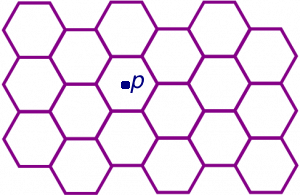
\includegraphics[width=2.5in]{Hex5.png}
 \end{center}
\caption{\small 除平移对称性外，蜂窝晶格还具有一个 12 阶对称群。
它可以等同于使某一六边形中心处一点 $p$ 保持不动的所有晶格对称性所构成的群。
（在相差平移群共轭的意义下，选取哪个六边形无关紧要。）晶格有一个 6 阶对称群，
由绕 $p$ 旋转 $2\pi n/6$（$n\in \Z$）的旋转组成。再补充以保持过 $p$ 的某条直线不动的反射，
便得到这个 12 阶群。\figloc{42}{58}}
 \label{Hex5}
\end{figure}

% [Tutor Note: 术语——这个 12 阶群是二面体群 $D_6$（点群 $C_{6v}$）：6 个绕 $p$ 的旋转与 6 个过 $p$ 的反射。$2\pi/6$ 旋转把 $K$ 映到 $K'$，故两个狄拉克点能量相同；保持各自狄拉克点不动的反射则保护其无能隙性（见 1.9 节 \ref{td} 的论证）。]
这是一个粗糙的模型，但石墨烯晶格具有许多对称性。除平移对称性之外，其对称性如下。
如图 \ref{Hex5} 所示，设 $p$ 为某个六边形的中心。
于是可以绕 $p$ 旋转 $2\pi/6$ 的任意整数倍，也可以沿过 $p$ 的各个轴作反射。例如，
可以找到一个把给定狄拉克点映到自身的反射——因此（回忆第 \ref{td} 节的讨论）只要扰动保持该
反射，我们在模型中求得的无能隙狄拉克模在此扰动下就仍然无能隙。还可以看出，
$2\pi/6$ 的旋转会交换两个狄拉克点，从而保证它们具有相同的能量。

% [Tutor Note: 易错——$H$ 无迹等价于 $A$、$B$ 两个子晶格的格点能相等，此时 $H$ 的本征值为 $\pm|1+e^{i\alpha}+e^{i\beta}|$，故除狄拉克点外每个动量处恰有一个态在零以下、一个在零以上；半满时费米能恰为狄拉克点的能量（本模型中取为零）。若 $A$、$B$ 在位能不等（例如石墨烯放在六方氮化硼衬底上），$H$ 出现非零迹，能隙打开。]
此外，由于（在理想化跃迁模型中）能带哈密顿量在狄拉克点之外处处迹为零，
所以在狄拉克点之外的每个动量处，恰有一个态的能量低于狄拉克点的能量、一个态的能量高于狄拉克点的能量。
因此，在半满时，费米能恰好就是狄拉克点的能量。正如第 \ref{bce} 节所讨论的，
对理想哈密顿量作任何足够小的、保持对称性的扰动之后，这一结论仍然成立。人们相信，
对于真空中、关掉依赖于自旋的力时的理想石墨烯晶体，
这一结论在真实世界中成立（图 \ref{symb}）。

% [Tutor Note: 易错——霍尔丹微扰给两个狄拉克点同号的质量，故每个自旋的总陈数为 $\frac12+\frac12=1$，计入自旋后量子霍尔系数为 $2\times(1/2+1/2)=2$；凯恩-梅勒（Kane-Mele）机制则因自旋-轨道耦合使自旋相反的电子获得相反符号的质量，净霍尔电导率为零而自旋霍尔电导率量子化，这才是二维拓扑绝缘体。]
特别地，人们相信，在没有依赖于自旋的力时，理想的石墨烯晶体具有无能隙的类狄拉克激发。
适当的、包含对称性破缺和／或依赖于自旋的力的扰动，可以给出各种各样的有能隙模型。
霍尔丹选择了一种破坏部分对称性的扰动，并给所有狄拉克模以同号的质量。计入自旋，
这给出量子霍尔系数 $2 \times (1/2+1/2)=2.$ 凯恩（Kane）与梅勒（Mele）\cite{KM}
分析了依赖于自旋的力的效应，得到了自旋量子霍尔效应，这正是二维拓扑绝缘体的萌芽。



  \begin{figure}
 \begin{center}
   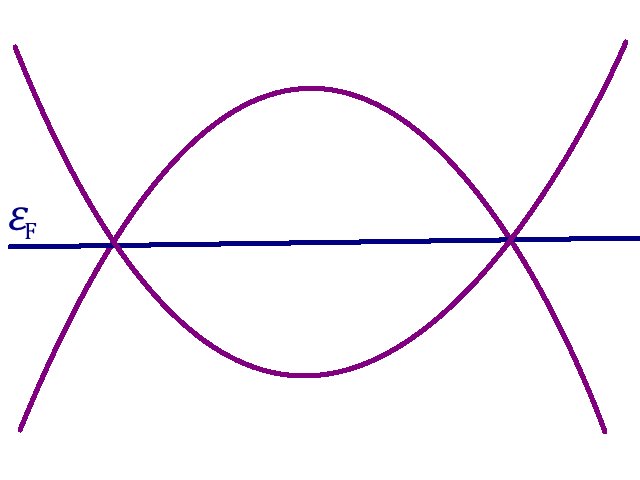
\includegraphics[width=2.5in]{SymBands2.png}
 \end{center}
\caption{\small 人们相信，真空中、关掉自旋-轨道力时，理想石墨烯晶体的费米能
恰好等于狄拉克点的能量。\figloc{43}{58}}
 \label{symb}
\end{figure}


% ======================================================================
%  参考文献（保留原文条目；仅修正明显的排版笔误，详见审校报告）
% ======================================================================
\clearpage
\addcontentsline{toc}{section}{参考文献}
\begin{thebibliography}{00}

\bibitem{KH}
M.~Z. Hasan and C.~L. Kane,
``Topological Insulators,''
Rev. Mod. Phys. {\bf 82} (2010) 3045.

\bibitem{ZQ}
Xiao-Liang Qi and Shou-Cheng Zhang,
``Topological Insulators And Superconductors,''
Rev. Mod. Phys. {\bf 83} (2011) 1057--1110, arXiv:1008.2026.

\bibitem{MZ}
M.~Z. Hasan and J.~E. Moore,
``Three-Dimensional Topological Insulators,''
arXiv:1011.5462,
Annu. Rev. Cond. Matt. Phys. {\bf 2} (2011) 55.

\bibitem{BH}
B.~A. Bernevig and T.~L. Hughes,
{\it Topological Insulators And Topological Superconductors}
(Princeton University Press, 2013).

\bibitem{Witten}
E.~Witten,
``Free Fermions And Topological Phases,''
arXiv:1508.04715.

\bibitem{Adler}
S.~Adler,
``Axial Vector Vertex In Spinor Electrodynamics,''
Phys. Rev. {\bf 177} (1969) 2426--2438.

\bibitem{BJ}
J.~S. Bell and R.~Jackiw,
``A PCAC Puzzle: $\pi^0\to\gamma\gamma$ In The Sigma Model,''
Nuovo Cimento {\bf A60} (1969) 47--61.

\bibitem{Herring}
C.~Herring,
``Accidental Degeneracy In The Energy Bands Of Crystals,''
Phys. Rev. {\bf 52} (1937) 365--373.

\bibitem{NN}
H.~B. Nielsen and M.~Ninomiya,
``A No-Go Theorem For Regularizing Chiral Fermions,''
Phys. Lett. {\bf B105} (1981) 219.

\bibitem{F}
D.~Friedan,
``A Proof Of The Nielsen-Ninomiya Theorem,''
Commun. Math. Phys. {\bf 85} (1982) 481.

\bibitem{TKNN}
D.~J. Thouless, M.~Kohmoto, M.~P. Nightingale, and M.~den Nijs,
``Quantized Hall Conductance In A Two-Dimensional Periodic Potential,''
Phys. Rev. Lett. {\bf 49} (1982) 405.

\bibitem{B}
M.~V. Berry,
``Quantal Phase Factors Accompanying Adiabatic Changes,''
Proc. Royal Soc. {\bf A392} (1984) 45--57.

\bibitem{ST}
P.~Schuster and N.~Toro,
``Continuous-Spin Particle Field Theory With Helicity Correspondence,''
Phys. Rev. {\bf D91} (2015) 025023, arXiv:1404.0675.

\bibitem{KM}
C.~L. Kane and E.~J. Mele,
``Quantum Spin Hall Effect In Graphene,''
Phys. Rev. Lett. {\bf 95} (2005) 226801.

\bibitem{WTVS}
X.~Wan, A.~M. Turner, A.~Vishwanath, and S.~Y. Savrasov,
``Topological Semimetal and Fermi-Arc Surface States in the Electronic Structure of
Pyrochlore Iridates,''
arXiv:1007.0016, Phys. Rev. {\bf B83} (2011) 205101.

\bibitem{FMK}
L.~Fu, C.~L. Kane, and E.~J. Mele,
``Topological Insulators In Three Dimensions,''
Phys. Rev. Lett. {\bf 98} (2007) 106803,
arXiv:cond-mat/0607699.

\bibitem{Mur}
S.~Murakami,
``Phase Transition Between the Quantum Spin Hall and Insulator Phases in 3D:
Emergence of a Topological Gapless Phase,''
New J. Phys. {\bf 9} (2007) 356,
arXiv:0710.0930.

\bibitem{KK}
L.~Fu and C.~L. Kane,
``Topology, Delocalization via Average Symmetry and the Symplectic Anderson Transition,''
Phys. Rev. Lett. {\bf 109} (2012) 246605,
arXiv:1208.3442.

\bibitem{YN}
B.-J. Yang and N.~Nagaosa,
``Classification of Stable Three-Dimensional Dirac Semimetals with Nontrivial Topology,''
arXiv:1404.0754,
Nature Communications {\bf 5} (2014) 4898.

\bibitem{ASSS}
J.~E. Avron, L.~Sadun, J.~Segert, and B.~Simon,
``Topological Invariants In Fermi Systems With Time-Reversal Invariance,''
Phys. Rev. Lett. {\bf 61} (1988) 1329--1332.

\bibitem{YZ}
S.~M. Young, S.~Zaheer, J.~C.~Y. Teo, and C.~L. Kane,
``Dirac Semimetal In Three Dimensions,''
Phys. Rev. Lett. {\bf 108} (2012) 140405.

\bibitem{YK}
S.~M. Young and C.~L. Kane,
``Dirac Semimetals In Two Dimensions,''
arXiv:1504.07977, Phys. Rev. Lett. {\bf 115} (2015) 126803.

\bibitem{Haldane}
F.~D.~M. Haldane,
``Model For A Quantum Hall Effect Without Landau Levels:
Condensed Matter Realization Of The `Parity Anomaly',''
Phys. Rev. Lett. {\bf 61} (1988) 2016--2018.

\bibitem{Wen}
X.-G. Wen,
``Topological Orders and Edge Excitations in FQH States,''
Adv. Phys. {\bf 44} (1995) 405, arXiv:cond-mat/9506066.

\bibitem{CH}
C.~G. Callan, Jr., and J.~A. Harvey,
``Anomalies And Fermion Zero-Modes On Strings And Domain Walls,''
Nucl. Phys. {\bf B250} (1985) 427.

\bibitem{Thouless}
D.~J. Thouless,
``Quantization Of Particle Transport,''
Phys. Rev. {\bf B27} (1983) 6083--6087.

\bibitem{Red}
N.~Redlich,
``Parity Violation And Gauge Noninvariance of the Effective Gauge Field Action In Three Dimensions,''
Phys. Rev. {\bf D29} (1984) 2366.

\bibitem{Semenoff}
A.~Niemi and G.~Semenoff,
``Anomaly-Induced Fermion Fractionization And Effective Actions In Odd-Dimensional Spacetimes,''
Phys. Rev. Lett. {\bf 51} (1983) 2077--2080.

\bibitem{JR}
R.~Jackiw and C.~Rebbi,
``Solitons With Fermion Number 1/2,''
Phys. Rev. {\bf D13} (1976) 3398.

\bibitem{Wallace}
P.~R. Wallace,
``The Band Theory Of Graphite,''
Phys. Rev. {\bf 71} (1947) 622.

\bibitem{Sem}
G.~Semenoff,
``Condensed Matter Simulation Of A Three-Dimensional Anomaly,''
Phys. Rev. Lett. {\bf 53} (1984) 2449.

\bibitem{GM}
D.~P. DiVincenzo and E.~J. Mele,
``Self-Consistent Effective Mass Theory For Intralayer Screening In Graphite Intercalation Compounds,''
Phys. Rev. {\bf B29} (1984) 1685--1694.

\end{thebibliography}


\end{document}
